\documentclass[11pt]{amsart}

\usepackage{macros}

\linespread{1.25}

\def\sAd{\sA{\rm d}}

\usepackage[final]{pdfpages}

\setcounter{tocdepth}{2}
\numberwithin{equation}{section}



\def\brian{\textcolor{blue}{BW: }\textcolor{blue}}
\def\owen{\textcolor{magenta}{OG: }\textcolor{magenta}}

\begin{document}
\title{Higher Kac-Moody algebras and symmetries of holomorphic field theories}

\author{Owen Gwilliam}
\address{Department of Mathematics and Statistics \\
Lederle Graduate Research Tower, 1623D \\
University of Massachusetts Amherst \\
710 N. Pleasant Street}
\email{gwilliam@math.umass.edu}

\author{Brian Williams}
\address{Department of Mathematics, 
Northeastern University \\ 
567 Lake Hall \\ 
Boston, MA 02115 \\ U.S.A.}
\email{br.williams@northeastern.edu}


\begin{abstract}
We introduce a higher dimensional generalization of the affine Kac-Moody algebra using the language of factorization algebras. 
In particular, on any complex manifold there is a factorization algebra of "currents" associated to any Lie algebra. 
We classify local cocycles of these current algebras, and compare them to central extensions of higher affine algebras recently proposed by Faonte-Hennion-Kapranov. 
A central goal of this paper is to witness higher Kac-Moody algebras as symmetries of a class of holomorphic quantum field theories. 
In particular, we prove a generalization of the free field realization of an affine Kac-Moody algebra and also develop the theory of $q$-characters for this class of algebras in terms of factorization homology.
Finally, we exhibit the ``large $N$" behavior of higher Kac-Moody algebras and their relationship to symmetries of non-commutative field theories. 
\end{abstract}

\maketitle
\thispagestyle{empty}

\newpage
\tableofcontents

\newpage

\section*{}

%\chapter{Local symmetries of holomorphic theories}\label{chap: symmetries}

The loop algebra $L\fg = \fg[z,z^{-1}]$, consisting of Laurent polynomials valued in a Lie algebra $\fg$,
admits a non-trivial central extension $\Hat{\fg}$ for each choice of invariant pairing on $\fg$.
This affine Lie algebra and its cousin, the Kac-Moody vertex algebra, are foundational objects in representation theory and conformal field theory. 
A natural question then arises: do there exists multivariable, or higher dimensional, generalizations of the affine Lie algebra and Kac-Moody vertex algebra? 

In this work, we pursue two independent yet related goals:
 
\begin{enumerate}
\item Use factorization algebras to study the (co)sheaf of Lie algebra-valued currents on complex manifolds, and their relationship to higher affine algebras;
\item Develop tools for understanding symmetries of {\em holomorphic field theory} in any dimension, that provide a systematic generalization of methods used in chiral conformal field theory on Riemann surfaces.
\end{enumerate}

Concretely, for every complex dimension $d$ and to every Lie algebra, we define a factorization algebra defined on all $d$-dimensional complex manifolds. 
There is also a version that works for an arbitrary principal bundle. 
When $d=1$, it is shown in \cite{CG1}, that this factorization algebra recovers the ordinary affine algebra by restricting the factorization algebra to the punctured complex line $C^*$. 
When $d > 1$, part of our main result is to show how the factorization algebra on $\CC^d \setminus \{0\}$ recovers a higher dimensional central extensions of $\fg$-valued functions on the punctured plane. 
A model for these ``higher affine algebras" has recently appeared in work of Faonte-Hennion-Kapranov \cite{FHK}, and we will give a systematic relationship between our approaches. 

By a standard procedure, there is a way of enhancing the affine algebra to a vertex algebra. 
The so-called Kac-Moody vertex algebra, as developed in \cite{IgorKM, KacVertex, BorcherdsVertex}, is important in its own right to representation theory and conformal field theory. 
In \cite{CG1} it is also shown how the holomorphic factorization algebra associated to a Lie algebra recovers this vertex algebra. 
The key point is that the OPE is encoded by the factorization product between disks embedded in $\CC$. 
Our proposed factorization algebra, then, provides a higher dimensional enhancement of this vertex algebra through the factorization product of balls or polydisks in $\CC^d$. 
This structure can be thought of as a holomorphic analog of an algebra over the operad of little $d$-disks.

It is the general philosophy of \cite{CG1,CG2} that every quantum field theory defines a factorization algebra of observables.
This perspective allows us to realize the higher Kac-Moody algebra inside of familiar higher dimensional field theories. 
In particular, this philosophy leads to higher dimensional analogs of free field realization via a quantum field theory called the $\beta\gamma$ system, which is defined on any complex manifold. 

In complex dimension one, a vertex algebra is a gadget associated to any conformal field theory that completely determines the algebra of local operators.  
More recently, vertex algebras have been extracted from higher dimensional field theories, such as $4$-dimensional gauge theories \cite{Beem1, Beem2}. 
A future direction, which we do not undertake here, would be to use these higher dimensional vertex algebras as a more refined invariant of the quantum field theory. 

Before embarking on our main results, we take some time to motivate higher dimensional current algebras from two different perspectives. 

\subsection*{A view from physics}

In conformal field theory, the Kac-Moody algebra appears as the symmetry of a system with an action by a Lie algebra. 
A generic example is a flavor symmetry of a field theory where the matter takes values in some representation.
In ordinary 2d chiral CFT, the central extension appears as the failure of the classical Lie bracket on $\fg$-valued currents to be compatible with the OPE. 
This is measured by the charge anomaly, which occurs as a $2$-point function in the CFT. 

This paper is concerned with symmetries for holomorphic theories in any complex dimension. 
Classically, the story is completely analogous to the ordinary picture in chiral CFT: for holomorphic theories, the action by a Lie algebra is enhanced to a symmetry by an infinite dimensional Lie algebra of currents on the $S^{2d-1}$-modes of the holomorphic theory. 
This current algebra is an algebraic version of the sphere mapping space $\Map(S^{2d-1}, \fg)$. 

In any dimension, there is a chiral charge anomaly for the class of holomorphic field theories that we study, which measures the failure of quantizing the classical symmetry. 
In complex dimension $2$ (real dimension $4$), for instance, the anomaly is a holomorphic version of the Adler-Bardeen-Jackiw anomaly \cite{Adler, BJ}.
In terms of supersymmetric field theory, the anomaly is the holomorphic twist of the Konishi anomaly \cite{Konishi}. 
For a general form of the anomaly in our situation, we refer to Section \ref{sec: qft}, where we consider a general class of theories with ``holomorphic matter". 

Throughout this paper, we use ideas and techniques from the Batalin-Vilkovisky formalism, as articulated by Costello, and from the theory of factorization algebras, following \cite{CG1,CG2}.
In this introduction, however, we will try to explain the key objects and constructions with a light touch,
in a way that does not require familiarity with that formalism,
merely comfort with basic complex geometry and ideas of quantum field theory.

A running example is the following version of the $\beta\gamma$ system.

Let $X$ be a complex $d$-dimensional manifold.
Let $G$ be a complex algebraic group, such as $GL_n(\CC)$, 
and let $P \to X$ be a holomorphic principal $G$-bundle.
Fix a finite-dimensional $G$-representation $V$ and let $V^\vee$ denote the dual vector space with the natural induced $G$-action.
Let $\cV \to X$ denote the holomorphic associated bundle $P \times^G V$, 
and let $\cV^! \to X$ denote the holomorphic bundle $K_X \otimes \cV^\vee$,
where $\cV^* \to X$ is the holomorphic associated bundle $P \times^G V^*$.
Note that there is a natural fiberwise pairing
\[
\langle-,-\rangle: \cV \otimes \cV^! \to K_X \footnote{The shriek denotes the Serre dual, $\sV^! = K_X \tensor V^\vee$.}
\]
arising from the evaluation pairing between $V$ and~$V^\vee$.

The field theory involves fields $\gamma$, for a smooth section of $\cV$, and $\beta$, for a smooth section of $\Omega^{0,d-1} \tensor \sV^\vee$.
Here, $\sV^\vee$ denotes the dual bundle. 
The action functional is
\[
S(\beta,\gamma) = \int_X \langle \beta, \dbar \gamma \rangle,
\]
so that the equations of motion are
\[
\dbar \gamma = 0 = \dbar \beta.
\]
Thus, the classical theory is manifestly holomorphic: it picks out holomorphic sections of $\cV$ and $\cV^!$ as solutions.

The theory also enjoys a natural symmetry with respect to $G$,
arising from the $G$-action on $\cV$ and $\cV^!$.
For instance, if $\dbar \gamma = 0$ and $g \in G$, then the section $g \gamma$ is also holomorphic.
In fact, there is a local symmetry as well.
Let ${\rm ad}(P) \to X$ denote the Lie algebra-valued bundle $P \times^G \fg \to X$ arising from the adjoint representation $\ad(G)$.
Then a holomorphic section $f$ of $\ad(P)$ acts on a holomorphic section $\gamma$ of $\cV$,
and 
\[
\dbar(f \gamma) =  (\dbar f) \gamma + f \dbar \gamma = 0,
\]
so that the sheaf of holomorphic sections of $\ad(P)$ encodes a class of local symmetries of this classical theory.

If one takes a BV/BRST approach to field theory, as we will in this paper,
then one works with a cohomological version of fields and symmetries.
For instance, it is natural to view the classical fields as consisting of the graded vector space of Dolbeault forms
\[
\gamma \in \Omega^{0,*}(X,\cV) \quad \text{and} \quad \beta \in \Omega^{0,*}(X, \cV^!) \cong \Omega^{d,*}(X, \cV^*),
\]
but using the same action functional, extended in the natural way.
As we are working with a free theory and hence have only a quadratic action,
the equations of motion are linear and can be viewed as equipping the fields with the differential $\dbar$.
In this sense, the sheaf $\cE$ of solutions to the equations of motion can be identified with the elliptic complex that assigns to an open set $U \subset X$, the complex
\[
\cE(U) = \Omega^{0,*}(U,\cV) \oplus \Omega^{0,*}(U, \cV^!),
\]
with $\dbar$ as the differential.
This dg approach is certainly appealing from the perspective of complex geometry,
where one routinely works with the Dolbeault complex of a holomorphic bundle.

It is natural then to encode the local symmetries in the same way.
Let $\sAd(P)$ denote the Dolbeault complex of ${\rm ad}(P)$ viewed as a sheaf.
That is, it assigns to the open set $U \subset X$, the dg Lie algebra 
\[
\sAd(P)(U) = \Omega^{0,*}(U,\ad(P))
\]
with differential $\dbar$ for this bundle.
By construction, $\sAd(P)$ acts on $\cE$.
In words, $\cE$ is a sheaf of dg modules for the sheaf of dg Lie algebra~$\sAd(P)$.

So far, we have simply lifted the usual discussion of symmetries to a dg setting,
using standard tools of complex geometry.
We now introduce a novel maneuver that is characteristic of the BV/factorization package of~\cite{CG1,CG2}.

The idea is to work with compactly supported sections of $\sAd(P)$, 
i.e., to work with the precosheaf $\sAd(P)_c$ of dg Lie algebras that assigns to an open $U$,
the dg Lie algebra
\[
\sAd(P)_c(U) = \Omega^{0,*}_c(U,\ad(P)).
\]
The terminology {\em precosheaf} encodes the fact that there is natural way to extend a section supported in $U$ to a larger open $V \supset U$ (namely, extend by zero),
and so one has a functor $\sAd(P) \colon {\rm Opens}(X) \to {\rm Alg}_{\rm Lie}$.

There are several related reasons to consider compact support.\footnote{In Section \ref{sec: fact} we extract factorization algebras from $\sAd(P)_c$,
and then extract associative and vertex algebras of well-known interest.
We postpone discussions within that framework till that section.}
First, it is common in physics to consider compactly-supported modifications of a field.
Recall the variational calculus, where one extracts the equations of motion by working with precisely such first-order perturbations.
Hence, it is natural to focus on such symmetries as well.
Second, one could ask how such compactly supported actions of $\sAd(P)$ affect observables.
More specifically, one can ask about the charges of the theory with respect to this local symmetry.\footnote{We remark that it is precisely this relationship with traditional physical terminology of currents and charges that led de Rham to use {\em current} to mean a distributional section of the de Rham complex.}
Third---and this reason will become clearer in a moment---the anomaly that appears when trying to quantize this symmetry are naturally local in $X$, and hence it is encoded by a kind of Lagrangian density $L$ on sections of $\sAd(P)$.
Such a density only defines a functional on compactly supported sections,
since when evaluated a noncompactly supported section $f$, the density $L(f)$ may be non-integrable.
Thus $L$ determines a central extension of $\sAd(P)_c$ as a precosheaf of dg Lie algebras,
but not as a sheaf.\footnote{We remark that to stick with sheaves, one must turn to quite sophisticated tools \cite{WittenGr, GetzlerGM, ManBeilSch} that can be tricky to interpret, much less generalize to higher dimension, whereas the cosheaf-theoretic version is quite mundane and easy to generalize, as we'll see.}

Let us sketch how to make these reasons explicit.
The first step is to understand how $\sAd(P)_c$ acts on the observables of this theory.

Modulo functional analytic issues,
we say that the observables of this classical theory are the commutative dg algebra
\[
(\Sym(\Omega^{0,*}(X,\cV)^* \oplus \Omega^{0,*}(X, \cV^!)^*), \dbar),
\]
i.e., the polynomial functions on $\cE(X)$.
More accurately, we work with a commutative dg algebra essentially generated by the continuous linear functionals on $\cE(X)$, 
which are compactly supported distributional sections of certain Dolbeault complexes ({\it aka} Dolbeault currents).
We could replace $X$ by any open set $U \subset X$, 
in which case the observables with support in $U$ arise from such distributions supported in $U$.
We denote this commutative dg algebra by $\Obs^{cl}(U)$.
Since observables on an open $U$ extend to observables on a larger open $V \supset U$,
we recognize that $\Obs^{cl}$ forms a precosheaf.

Manifestly, $\sAd(P)_c(U)$ acts on $\Obs^{cl}(U)$,
by precomposing with its action on fields.
Moreover, these actions are compatible with the extension maps of the precosheaves,
so that $\Obs^{cl}$ is a module for $\sAd(P)_c$ in precosheaves of cochain complexes.
This relationship already exhibits why one might choose to focus on $\sAd(P)_c$,
as it naturally intertwines with the structure of the observables.

But Noether's theorem provides a further reason,
when understood in the context of the BV formalism.
The idea is that $\Obs^{cl}$ has a Poisson bracket $\{-,-\}$ of degree 1
(although there are some issues with distributions here that we suppress for the moment).
Hence one can ask to realize the action of $\sAd(P)_c$ via the Poisson bracket.
In other words, we ask to find a map of (precosheaves of) dg Lie algebras
\[
J \colon \sAd(P)_c \to \Obs^{cl}[-1]
\]
such that for any $f \in \sAd(P)_c(U)$ and $F \in \Obs^{cl}(U)$,
we have
\[
f \cdot F = \{J(f),F\}.
\]
Such a map would realize every symmetry as given by an observable,
much as in Hamiltonian mechanics.

In this case, there is such a map:
\[
J(f)(\gamma,\beta) = \int_U \langle\beta, f \gamma\rangle.
\]
This functional is local, and it is natural to view it as describing the ``minimal coupling'' between our free $\beta\gamma$ system and a kind of gauge field implicit in $\sAd(P)$.
This construction thus shows again that it is natural to work with compactly supported sections of $\sAd(P)$,
since it allows one to encode the Noether map in a natural way.
We call $\sAd(P)_c$ the Lie algebra of {\em classical currents} as we have explained how, via $J$, we realize these symmetries as classical observables.

\begin{rmk}
We remark that it is not always possible to produce such a Noether map,
but the obstruction always determines a central extension of $\sAd(P)_c$ as a precosheaf of dg Lie algebras,
and one can then produce such a map to the classical observables.
\end{rmk}

In the BV formalism, quantization amounts to a deformation of the differential on $\Obs^{cl}$,
where the deformation is required to satisfy certain properties.
Two conditions are preeminent:
\begin{itemize}
\item the differential satisfies a {\em quantum master equation}, which ensures that $\Obs^q(U)[-1]$ is still a dg Lie algebra via the bracket,\footnote{Again, we are suppressing---for the moment important---issues about renormalization, which will play a key role when we get to the real work.} and
\item it respects support of observables so that $\Obs^q$ is still a precosheaf.
\end{itemize}
The first condition is more or less what  BV quantization means, 
whereas the second is a version of the locality of field theory.

We can now ask whether the Noether map $J$ determines a map of precosheaves of dg Lie algebras from $\sAd(P)_c$ to $\Obs^q[-1]$.
Since the Lie bracket has not changed on the observables, 
the only question is where $J$ is a cochain map for the new differential $\d^q$
If we write $\d^q = \d^{cl} + \hbar \Delta$,\footnote{By working with smeared observables, one really can work with the naive BV Laplacian $\Delta$. Otherwise, one must take a little more care.} then 
\[
[\d,J] = \hbar \Delta \circ J.
\]
Naively---i.e., ignoring renormalization issues---this term is the functional $ob$ on $\sAd(P)_c$ given 
\[
ob(f) = \int \langle f K_\Delta \rangle,
\]
where $K_\Delta$ is the integral kernel for the identity with respect to the pairing $\langle-,-\rangle$.
(It encodes a version of the trace of $f$ over $\cE$.)
This obstruction should resemble standard anomalies.

This functional $ob$ is a cocycle in Lie algebra cohomology for $\sAd(P)$ and hence determines a central extension $\widehat{\sAd(P)}_c$ as precosheaves of dg Lie algebras.
It is the Lie algebra of {\em quantum} currents, as there is a lift of $J$ to a map $J^q$ out of this extension to the quantum observables.

\subsection*{A view from geometry}

There is also a strong motivation for the algebras we consider from the perspective of the geometry of mapping spaces. 
There is an embedding $\fg[z,z^{-1}] \hookrightarrow C^\infty(S^1) \tensor \fg = {\rm Map}(S^1, \fg)$, induced by the embedding of algebraic functions on punctured affine line inside of smooth functions on $S^1$. 
Thus, a natural starting point for $d$-dimensional affine algebras is the ``sphere algebra" 
\beqn\label{mapping space}
{\rm Map}(S^{2d-1}, \fg) ,
\eeqn
where we view $S^{2d-1}$ sitting inside punctured affine space~$\pAA^d = \CC^d \setminus \{0\}$. 

When $d=1$, affine algebras are given by extensions $L\fg$ prescribed by a $2$-cocycle involving the algebraic residue pairing. 
Note that this cocycle is {\em not} pulled back from any cocycle on $\sO_{\rm alg}(\AA^1) \tensor \fg = \fg[z]$. 
%Now, consider algebraic functions on the punctured $d$-dimensional affine space $\AA^{d \times}$.

When $d > 1$, Hartog's theorem implies that the space of holomorphic functions on punctured affine space is the same as the space of holomorphic functions on affine space.
The same holds for algebraic functions, so that $\sO_{\rm alg}(\pAA^{d}) \tensor \fg = \sO_{\rm alg}(\AA^d) \tensor \fg$. 
In particular, the naive generalization $\sO_{\rm alg}(\pAA^{d}) \tensor \fg$ of (\ref{mapping space}) has no interesting central extensions. 
However, in contrast with the punctured line, the punctured affine space $\pAA^{d}$ has interesting higher cohomology. 

The key idea is to replace the commutative algebra $\cO_{\rm alg}(\pAA^{d})$ by the derived space of functions $\RR \Gamma(\pAA^{d}, \sO_{\rm alg})$. 
This complex has interesting cohomology and leads to nontrivial extensions of the Lie algebra object $\RR \Gamma(\pAA^{d}, \sO) \tensor \fg$, as well as its Dolbeault model $\Omega^{0,*}(\pAA^d) \tensor \fg$.
Faonte-Hennion-Kapranov \cite{FHK} have provided a systematic exploration of this situation.

Our starting point is to work in the style of complex differential geometry and use the sheaf of $\fg$-valued Dolbeault forms $\Omega^{0,*}(X, \fg)$, defined on any complex manifold $X$. 
We deem this sheaf of dg Lie algebras---or rather its cosheaf version $\sG_X = \Omega^{0,*}_c(X, \fg)$---the {\em holomorphic $\fg$-valued currents} on~$X$. 
We will see that there exists cocycls on this sheaf of dg Lie algebras that give rise to interesting extensions of the factorization algebra~$\clieu_*\sG_X$,
which serve as our model for a higher dimensional Kac-Moody algebra. 
Section~\ref{sec:FHK} is devoted to relating our construction to that in~\cite{FHK}.

A novel facet of this paper is that we enhance this Lie algebraic object to a {\em factorization algebra} on the manifold~$X$
by working with whe Lie algebra chains $\clieu_*\sG_X$ of this cosheaf.
It serves as a higher dimensional analog of the chiral enveloping algebra of $\fg$ introduced by Beilinson and Drinfeld \cite{BD}, 
and it yields a higher dimensional generalization of the vertex algebra of a Kac-Moody algebra. 

Analogs of important objects over Riemann surfaces arise from this new construction.
For instance, we obtain a version of bundles of conformal blocks from our higher Kac-Moody algebras:
factorization algebras are local-to-global objects, and one can take the global sections
(sometimes called the factorization or chiral homology).
In this paper we explicitly examine the factorization homology on Hopf manifolds,
which provide a systematic generalization of elliptic curves 
in the sense that their underlying manifolds are diffeomorphic to $S^1 \times S^{2d-1}$.
Due to the appearance $S^1$, one finds connections with traces.
As one might hope, these Hopf manifolds form moduli and so one can obtain, in principle, generalizations of $q$-character formulas.
(Giving explicit formulas is deferred to a future work.)

Another key generalization is given by natural determinant lines on moduli of bundles.
Any finite-dimensional representation $V$ of the Lie algebra $\fg$ determines a line bundle over the moduli of bundles on a complex manifold~$X$: 
take the determinant of the Dolbeault cohomology of the associated holomorphic vector bundle $\cV$ over~$X$.
In \cite{FHK} they use derived algebraic geometry to provide a higher Kac-Moody uniformization for complex $d$-folds and discuss these determinant lines.
We offer a complementary perspective: such a determinant line appears as the global sections of a certain factorization algebra on $X$ determined by the vector bundle~$\cV$.
That is, there is another factorization algebra whose bundle of conformal blocks encodes this determinant.
We construct this factorization algebra as observables of a quantum field theory,
as generalizations of the $bc$ and $\beta\gamma$ systems.\footnote{To be more precise, our construction uses formal derived geometry and works on the formal neighborhood of any point on the moduli of bundles. 
Properly taking into account the global geometry would require more discussion.}
In short, by combining \cite{FHK} with our results, 
there seems to emerge a systematic, higher-dimensional extension of the beautiful, rich dialogue between representation theory of infinite-dimensional Lie algebras, complex geometry, and conformal field theory.

%The key idea is that we replace the commutative algebra $\sO^{alg}(\pAA^{d})$ by the derived space of sections $\RR \Gamma(\pAA^{d}, \sO)$. 
%This complex has interesting cohomology and leads to nontrivial extensions of the dg Lie algebra $\RR \Gamma(\pAA^{d}, \sO) \tensor \fg$, or its Dolbeault model $\Omega^{0,*}(\pAA^d)$.
%Further, there is a tangential Dolbeault complex of the $(2d-1)$-sphere inside of the Dolbeault complex of $\CC^d \setminus \{0\}$:
%\[
%\Omega_b^{0,*}(S^{2d-1}) \subset \Omega^{0,*}(\pAA^d) .
%\]
%See \cite{DragomirTomassini} for details on the definition of $\Omega_b^{0,*}(S^{2d-1})$. 
%The degree zero part of $\Omega_b^{0,*}(S^{2d-1})$ is $C^\infty(S^{2d-1})$, and we can view it as a derived enhancement of the mapping space in (\ref{mapping space}). 
%The key fact is that the dg Lie algebra $\Omega^{0,*}(S^{2d-1}) \tensor \fg$ {\em does} have nontrivial central extensions. 
%
%Our starting point is to step back, and consider the full sheaf of $\fg$-valued Dolbeualt forms $\Omega^{0,*}(X, \fg)$ defined on any complex manifold $X$. 
%We deem this sheaf of dg Lie algebras, or rather its cosheaf version $\sG_X := \Omega^{0,*}_c(X, \fg)$, the {\em holomorphic $\fg$-valued currents} on $X$. 
%The Lie algebra homology, $\clieu_*\sG_X$, of this cosheaf determines the structure of a {\em factorization algebra} on the manifold $X$.
%It serves as a higher dimensional analog of the chiral enveloping algebra of $\fg$ introduced by Beilinson-Drinfeld \cite{BD}, and will or model for the higher dimensional Kac-Moody algebra. 

%\begin{thm}\label{thm sphere alg} The associative algebra $U(\Hat{\fg}_{d,\theta})$ determines a locally constant factorization algebra on the real one-manifold $\RR$ that we denote $U(\Hat{\fg}_{d,\theta})^{fact}$. 
%Moreover, there is an injective dense map of factorization algebras on $\RR$:
%\[
%\Phi^{S^{2d-1}} : \left(U \Hat{\fg}_{d,\theta} \right)^{fact} \to r_*\left(\sF^{\CC^d \setminus \{0\}}_{\fg,\theta} \right)  .
%\]
%where the right-hand side is the push-forward of the Kac-Moody factorization algebra on $\CC^{d}\setminus \{0\}$ along the radial projection map.
%\end{thm}

%In the final part of this section we specialize to the manifold $X = (\CC \setminus \{0\})^d$. 
%Note that when $d=1$ this is the same as the algebra above, but for $d>1$ this factorization algebra has a different flavor. 
%We will show how to extract the data of an $E_d$-algebra from this configuration, and discuss its role in the theory of higher dimensional vertex algebras. 

%In a similar way in Section \ref{sec: ...} we will see how the Kac-Moody factorization algebra on $(\CC \setminus \{0\})^d$ are related to extensions of higher loop Lie algebras
%\[
%L^d \fg = L ( \cdots (L \fg) \cdots ) = {\rm Map}(S^{1} \times S^1 , \fg).
%\]

%\[
%\cA_{d, \fg,\theta} := \bigoplus_{k \in \ZZ} r_*\left(\sF^{\CC^d}_{\fg,\theta} |_{\CC^d \setminus 0} \right) ^{(k)} \subset r_*\left(\sF^{\CC^d}_{\fg,\theta} |_{\CC^d \setminus 0} \right) .
%\]
%\end{thm}

%\begin{dfn} Fix an element $\theta \in \Sym^{d+1}(\fg)^{\fg}$. 
%Let $\Hat{\fg}_{d,\theta}$ be the $L_\infty$ central extension
%\[
%\CC \to \Hat{\fg}_{d,\theta} \to A_d \tensor \fg
%\]
%determined by the degree two cocycle $\theta_{\rm FHK} \in \clie^*(A_d \tensor \fg)$ defined by
%\[
%\theta_{\rm FHK}(a_0\tensor X_0,\dots,a_d\tensor X_d) = \Reszero \left(a_0 \wedge \d a_1 \wedge \cdots \wedge \d a_d \right) \theta(X_0,\ldots,X_d)
%\]
%where $a_i \tensor X_i \in A_d \tensor \fg$. 
%\end{dfn}

\subsection*{Acknowledgements}

We have intermittently worked on this project for several years,
and our collaboration benefited from shared time at the Max Planck Institute for Mathematics in Bonn, Germany and the Perimeter Institute for Physics in Waterloo, Canada.
We thank both institutions for their support and for their convivial atmosphere.
Most of these results appeared first in Chapter 4 of the second author's Ph.D. thesis \cite{BWthesis},
of which this paper is a revised and enhanced version. 
The second author would therefore like to thank Northwestern University, where he received support as a graduate student whilst most of this work took place.
In addition, the second author enjoyed support as a graduate student research fellow under NSF Award DGE-1324585. 

In addition to institutional support, we received guidance and feedback from Kevin Costello, Giovanni Faonte, Benjamin Hennion, and Mikhail Kapranov. Thank you!

%Infinitesimally speaking, a symmetry is encoded by the action of a Lie algebra.
%For the holomorphic gauge symmetry this will become a sort of current algebra which is equivalent to holomorphic functions on the complex manifold with values in a Lie algebra.
%For the holomorphic diffeomorphisms this Lie algebra is that of holomorphic vector fields.
%Locality implies that this actually extends to a symmetry by a sheafy version of a Lie algebra. 
%The precise sheafy version we mean is called a {\em local Lie algebra}, which we will recall in the main body of the text. 
%To every local Lie algebra we can assign a factorization algebra through the so-called enveloping factorization algebra:
%\[
%\mathbb{U} : {\rm Lie}_X \to {\rm Fact}_X .
%\]
%Here, ${\rm Lie}_X$ is the category of local Lie algebras.
%By this construction, we see that the Lie algebra of symmetries of a theory define a factorization algebra on the manifold where the theory lives. 
%
%One compelling reason for constructing a factorization algebra model for Lie algebras encoding the symmetries of a theory is that it allows one to consider universal versions of such objects.
%There is a variation of the definition of a factorization algebra that lives, in some sense, on the entire category of manifolds (or complex manifolds). 
%Such a perspective has been developed in great generality by Ayala-Francis in \cite{AFTopMan}.
%In the case of the symmetry by a current algebra on Riemann surfaces a universal version of the Kac-Moody has been studied in \cite{CG1}.
%For the case of conformal symmetry our work in \cite{BWVir} provides a factorization algebra lift of the ordinary Virasoro vertex algebra that exists uniformly on the site of Riemann surfaces. 
%In this chapter, we extend each of these objects to arbitrary complex dimensions.
%Our formulation lends itself to an explicit computation of the factorization homology along certain complex manifolds, for which we will focus on a class of examples called {\em Hopf manifolds}.
%
%For this reason, an essential aspect of studying the local symmetries of holomorphic field theories we mentioned above is to characterize the possible cocycles that give rise to central extensions. 
%As we have already mentioned, for vector fields in complex dimension one this is related to the central charge and the central extension of the Witt algebra (vector fields on the circle) known as the Virasoro Lie algebra.
%In the case of a current algebra associated to a Lie algebra, central extensions are related to the {\em level} and the corresponding central extensions are called affine algebras. 

%\begin{thm}
%Let $V$ be a finite dimensional $\fg$-module and $X$ any compact affine complex manifold. 
%There exists a BV quantization of the $\beta\gamma$-system on $X$ with values in $V$ that is equivariant for the local Lie algebra $\fg^X$. 
%Moreover, the first Chern class of the line bundle on $B \fg^X$ defined by the factorization homology of the quantization is equal to
%\[
%c_1(\Obs^\q(X)) = C \ch_{d+1}(V) \in \Sym^{d+1}(\fg^\vee)^\fg 
%\]
%where $C$ is some nonzero number.
%\end{thm}

\section{Lie algebras of currents}

\subsection{Motivational discussion}

\owen{I'm just letting it flow. This paragraph might profitably go elsewhere.}

Our focus in this paper is upon field theories that depend upon complex geometry, 
specifically upon the symmetries they possess.
Our overarching goal is to explain tools for understanding such symmetries that provide a systematic generalization of methods used in chiral conformal field theory on Riemann surfaces,
notably the Kac-Moody vertex algebras.
These tools will use ideas and techniques from the Batalin-Vilkovisky formalism, as articulated by Costello, and factorization algebras, following \cite{CG1,CG2}.
In this subsection, however, we will try to explain the key objects and constructions with a light touch,
in a way that does not require familiarity with that formalism,
merely comfort with basic complex geometry and ideas of quantum field theory.

\subsubsection{}

A running example is the following version of the $\beta\gamma$ system.

Let $X$ be a complex $d$-dimensional manifold.
Let $G$ be a complex algebraic group, such as $GL_n(\CC)$, 
and let $P \to X$ be a holomorphic principal $G$-bundle.
Fix a finite-dimensional $G$-representation $V$ and let $V^*$ denote the dual vector space with the natural induced $G$-action.
Let $\cV \to X$ denote the holomorphic associated bundle $P \times^G V$, 
and let $\cV^! \to X$ denote the holomorphic bundle $K_X \otimes \cV^*$,
where $\cV^* \to X$ is the holomorphic associated bundle $P \times^G V^*$.
Note that there is a natural fiberwise pairing
\[
\langle-,-\rangle: \cV \otimes \cV^! \to K_X
\]
arising from the evaluation pairing between $V$ and~$V^*$.

The field theory involves fields $\gamma$, for a smooth section of $\cV$, and $\beta$, for a smooth section of $\cV^!$.
\owen{I need to adjust where $\beta$ lives in a way depending on dimension $d$.}
The action functional is
\[
S(\beta,\gamma) = \int_X \langle \beta, \dbar \gamma \rangle,
\]
so that the equations of motion are
\[
\dbar \gamma = 0 = \dbar \beta.
\]
Thus, the classical theory is manifestly holomorphic: it picks out holomorphic sections of $\cV$ and $\cV^!$ as solutions.

The theory also enjoys a natural symmetry with respect to $G$,
arising from the $G$-action on $\cV$ and $\cV^!$.
For instance, if $\dbar \gamma = 0$ and $g \in G$, then the section $g \gamma$ is also holomorphic.
In fact, there is a local symmetry as well.
Let $\ad(P) \to X$ denote the Lie algebra-valued bundle $P \times^G \fg \to X$ arising from the adjoint representation $\ad(G)$.
Then a holomorphic section $f$ of $\ad(P)$ acts on a holomorphic section $\gamma$ of $\cV$,
and 
\[
\dbar(f \gamma) =  (\dbar f) \gamma + f \dbar \gamma = 0,
\]
so that the sheaf of holomorphic sections of $\ad(P)$ encodes a class of local symmetries of this classical theory.

\subsubsection{}

If one takes a BV/BRST approach to field theory, as we will in this paper,
then one works with a cohomological version of fields and symmetries.
For instance, it is natural to view the classical fields as consisting of the graded vector space of Dolbeault forms
\[
\gamma \in \Omega^{0,*}(X,\cV) \quad \text{and} \quad \beta \in \Omega^{0,*}(X, \cV^!) \cong \Omega^{d,*}(X, \cV^*),
\]
but using the same action functional, extended in the natural way.
As we are working with a free theory and hence have only a quadratic action,
the equations of motion are linear and can be viewed as equipping the fields with the differential $\dbar$.
In this sense, the sheaf $\cE$ of solutions to the equations of motion can be identified with the elliptic complex that assigns to an open set $U \subset X$, the complexe
\[
\cE(U) = \Omega^{0,*}(U,\cV) \oplus \Omega^{0,*}(U, \cV^!),
\]
with $\dbar$ as the differential.
This dg approach is certainly appealing from the perspective of complex geometry,
where one routinely works with the Dolbeault complex of a holomorphic bundle.

It is natural then to encode the local symmetries in the same way.
Let $\cAd(P)$ denote the Dolbeault complex of $\ad(P)$ viewed as a sheaf.
That is, it assigns to the open set $U \subset X$, the dg Lie algebra 
\[
\cAd(P)(U) = \Omega^{0,*}(U,\ad(P))
\]
with differential $\dbar$ for this bundle.
By construction, $\cAd(P)$ acts on $\cE$.
In words, $\cE$ is a sheaf of dg modules for the sheaf of dg Lie algebra~$\cAd(P)$.

\subsubsection{}

So far, we have simply lifted the usual discussion of symmetries to a dg setting,
using standard tools of complex geometry.
We now introduce a novel maneuver that is characteristic of the BV/factorization package of~\cite{CG1,CG2}.

The idea is to work with compactly supported sections of $\cAd(P)$, 
i.e., to work with the precosheaf $\cAd(P)_c$ of dg Lie algebras that assigns to an open $U$,
the dg Lie algebra
\[
\cAd(P)_c(U) = \Omega^{0,*}_c(U,\ad(P)).
\]
The terminology {\em precosheaf} encodes the fact that there is natural way to extend a section supported in $U$ to a larger open $V \supset U$ (namely, extend by zero),
and so one has a functor $\cAd(P) \colon {\rm Opens}(X) \to {\rm Alg}_{\rm Lie}$.

There are several related reasons to consider compact support.\footnote{In Section \ref{sec: fact} we extract factorization algebras from $\cAd(P)_c$,
and then extract associative and vertex algebras of well-known interest.
We postpone discussions within that framework till that section.}
First, it is common in physics to consider compactly-supported modifications of a field.
Recall the variational calculus, where one extracts the equations of motion by working with precisely such first-order perturbations.
Hence, it is natural to focus on such symmetries as well.
Second, one could ask how such compactly supported actions of $\cAd(P)$ affect observables.
More specifically, one can ask about the charges of the theory with respect to this local symmetry.\footnote{We remark that it is precisely this relationship with traditional physical terminology of currents and charges that led de Rham to use {\em current} to mean a distributional section of the de Rham complex.}
Third---and this reason will become clearer in a moment---the anomaly that appears when trying to quantize this symmetry are naturally local in $X$, and hence it is encoded by a kind of Lagrangian density $L$ on sections of $\cAd(P)$.
Such a density only defines a functional on compactly supported sections,
since when evaluated a noncompactly supported section $f$, the density $L(f)$ may be non-integrable.
Thus $L$ determines a central extension of $\cAd(P)_c$ as a precosheaf of dg Lie algebras,
but not as a sheaf.\footnote{We remark that to stick with sheaves, one must turn to quite sophisticated tools \cite{WittenGr,GetzlerGM,ManBeilSch} that can be tricky to interpret, much less generalize to higher dimension, whereas the cosheaf-theoretic version is quite mundane and easy to generalize, as we'll see.}

\subsubsection{}

Let us sketch how to make these reasons explicit.
The first step is to understand how $\cAd(P)_c$ acts on the observables of this theory.

Modulo functional analytic issues,
we say that the observables of this classical theory are the commutative dg algebra
\[
(\Sym(\Omega^{0,*}(X,\cV)^* \oplus \Omega^{0,*}(X, \cV^!)^*), \dbar),
\]
i.e., the polynomial functions on $\cE(X)$.
More accurately, we work with a commutative dg algebra essentially generated by the continuous linear functionals on $\cE(X)$, 
which are compactly supported distributional sections of certain Dolbeault complexes ({\it aka} Dolbeault currents).
We could replace $X$ by any open set $U \subset X$, 
in which case the observables with support in $U$ arise from such distributions supported in $U$.
We denote this commutative dg algebra by $\Obs^{cl}(U)$.
Since observables on an open $U$ extend to observables on a larger open $V \supset U$,
we recognize that $\Obs^{cl}$ forms a precosheaf.

Manifestly, $\cAd(P)_c(U)$ acts on $\Obs^{cl}(U)$,
by precomposing with its action on fields.
Moreover, these actions are compatible with the extension maps of the precosheaves,
so that $\Obs^{cl}$ is a module for $\cAd(P)_c$ in precosheaves of cochain complexes.
This relationship already exhibits why one might choose to focus on $\cAd(P)_c$,
as it naturally intertwines with the structure of the observables.

But Noether's theorem provides a further reason,
when understood in the context of the BV formalism.
The idea is that $\Obs^{cl}$ has a Poisson bracket $\{-,-\}$ of degree 1
(although there are some issues with distributions here that we suppress for the moment).
Hence one can ask to realize the action of $\cAd(P)_c$ via the Poisson bracket.
In other words, we ask to find a map of (precosheaves of) dg Lie algebras
\[
J \colon \cAd(P)_c \to \Obs^{cl}[-1]
\]
such that for any $f \in \cAd(P)_c(U)$ and $F \in \Obs^{cl}(U)$,
we have
\[
f \cdot F = \{J(f),F\}.
\]
Such a map would realize every symmetry as given by an observable,
much as in Hamiltonian mechanics.

In this case, there is such a map:
\[
J(f)(\gamma,\beta) = \int_U \langle\beta, f \gamma\rangle.
\]
This functional is local, and it is natural to view it as describing the ``minimal coupling'' between our free $\beta\gamma$ system and a kind of gauge field implicit in $\cAd(P)$.
\owen{This is a little misleading, given the nature of the forms, but I think it is fixable.}
This construction thus shows again that it is natural to work with compactly supported sections of $\cAd(P)$,
since it allows one to encode the Noether map in a natural way.
We call $\cAd(P)_c$ the Lie algebra of {\em classical currents} as we have explained how, via $J$, we realize these symmetries as classical observables.

\begin{rmk}
We remark that it is not always possible to produce such a Noether map,
but the obstruction always determines a central extension of $\cAd(P)_c$ as a precosheaf of dg Lie algebras,
and one can then produce such a map to the classical observables.
\end{rmk}

\subsubsection{}

In the BV formalism, quantization amounts to a deformation of the differential on $\Obs^{cl}$,
where the deformation is required to satisfy certain properties.
Two conditions are preeminent:
\begin{itemize}
\item the differential satisfies a {\em quantum master equation}, which ensures that $\Obs^q(U)[-1]$ is still a dg Lie algebra via the bracket,\footnote{Again, we are suppressing---for the moment important---issues about renormalization, which will play a key role when we get to the real work.} and
\item it respects support of observables so that $\Obs^q$ is still a precosheaf.
\end{itemize}
The first condition is more or less what  BV quantization means, 
whereas the second is a version of the locality of field theory.

We can now ask whether the Noether map $J$ determines a map of precosheaves of dg Lie algebras from $\cAd(P)_c$ to $\Obs^q[-1]$.
Since the Lie bracket has not changed on the observables, 
the only question is where $J$ is a cochain map for the new differential $\d^q$
If we write $\d^q = \d^{cl} + \hbar \Delta$,\footnote{By working with smeared observables, one really can work with the naive BV Laplacian $\Delta$. Otherwise, one must take a little more care.} then 
\[
[\d,J] = \hbar \Delta \circ J.
\]
Naively---i.e., ignoring renormalization issues---this term is the functional $ob$ on $\cAd(P)_c$ given 
\[
ob(f) = \int \langle f K_\Delta \rangle,
\]
where $K_\Delta$ is the integral kernel for the identity with respect to the pairing $\langle-,-\rangle$.
(It encodes a version of the trace of $f$ over $\cE$.)
This obstruction should resemble standard anomalies.
\owen{Is that transition too abrupt? Should we provide an example?}

This functional $ob$ is a cocycle in Lie algebra cohomology for $\cAd(P)$ and hence determines a central extension $\widehat{\cAd(P)}_c$ as precosheaves of dg Lie algebras.
It is the Lie algebra of {\em quantum} currents, as there is a lift of $J$ to a map $J^q$ out of this extension to the quantum observables.

\subsection{Definitions}

We now introduce some definitions that aim to capture the abstract structure of the example just discussed.

\subsubsection{}

It will be convenient to generalize Lie algebras to $L_\infty$ algebras,
which involve multilinear brackets that satisfy higher versions of the Jacobi relation up to homotopy.

\owen{Just wanted to mention that your original definition of local Lie algebra was a little misleading, because it used $n \in \ZZ$ (not just positive integers) and said $\ell_n: \sL^{\otimes n} \to \sL[2-n]$. This tensor product might mislead people into thinking you mean tensor of sheaves of $C^\infty$-modules, which isn't correct. }

\begin{dfn} 
A {\em local $L_\infty$ algebra} on $X$ is the following data:
\begin{itemize}
\item[(i)] a $\ZZ$-graded vector bundle $L$ on $X$, whose sheaf of smooth sections we denote $\sL^{sh}$, and
\item[(ii)] for each positive integer $n$, a polydifferential operator in $n$ inputs
\ben
\ell_n : \underbrace{\sL^{sh} \times \cdots \times \sL^{sh}}_{\text{$n$ times}} \to \sL[2-n]
\een
\end{itemize}
such that the collection $\{\ell_n\}_{n \in \NN}$ satisfy the conditions of an $L_\infty$ algebra.
Thus $\sL^{sh}$ is a sheaf of $L_\infty$ algebras. 
\end{dfn}

In practice, we prefer to work with the compactly supported sections of $L$,
as explained in \owen{cross ref}, for which we reserve the more succinct notation~$\sL$.

\begin{dfn}
Given a local $L_\infty$ algebra $\sL$ on $X$, 
let $\sL$ denote the precosheaf of $L_\infty$ algebras that assigns compactly supported sections of $L$ to each open of~$X$.
\end{dfn}

We typically refer to the local $L_\infty$ algebra $(L, \{\ell_n\})$ by $\sL$. 
We will often use local {\em Lie} algebra, especially if $\sL$ is a precosheaf of dg Lie algebras and hence has trivial~$\ell_{n \geq 3}$.

\begin{eg}
Our favorite example, of course, arises from the adjoint bundle $\ad{P} \to X$ associated to a holomorphic principal $G$-bundle $P \to X$. 
We will hereafter use $\cAd(P)$ to denote the compactly supported sections of Dolbeault complex of $\ad{P}$.
\owen{Is that too confusing?}
\end{eg}

\begin{eg}
Another key local Lie algebra makes sense on an arbitrary complex $d$-fold.
Let $\fg$ be an ordinary Lie algebra, such as ${\frak{s}\frak{l}}_n$.
Let
\[
\sG^{sh} = \Omega^{0,*} \otimes \fg,
\]
which is a sheaf of dg Lie algebras on the category of complex $d$-folds and local biholomorphisms,\footnote{A biholomorphism is a map $\phi: X \to Y$ that is biijective and both $\phi$ and $\phi^{-1}$ are holomorphic. A {\em local} biholomorphism means a map $\phi: X \to Y$ such that for every point $x \in X$ has a neighborhood on which $\phi$ is a biholomorphism.
\owen{Not sure what you think of burying this in a footnote, but it seems tangential and not worth elaborating on in the main text.}}
and $\sG$ to denote $\Omega^{0,*}_c \otimes \fg$.
We use $\sG|_X$ to denote the restriction of $\sG$ to a fixed complex $d$-fold~$X$.
\end{eg}

Much of the rest of the section is devoted to constructing and analyzing various cocycles and extensions,
so we postpone further examples.

\subsubsection{}

We are interested in a certain class of central extensions of such an~$\sL_c$.

\begin{dfn}
A {\em local functional} on $\sL$ of cohomological degree $k$ is \owen{yuck} 
\end{dfn}

The graded vector space of local functionals is a subcomplex of $\clie^*(\sL_c)$, 
the naive Lie algebra cochains of $\sL_c$.
Let $\cloc^*(\sL)$ denote this cochain complex, as explained in detail in \owen{give precise citation}.
The differential is, in essence, just precomposition with the polydifferentials defining the brackets of~$\sL$.\footnote{Altogether $\cloc^*(\sL)$ is just a version of diagonal Gelfand-Fuks cohomology for this kind of Lie algebra.} 

\begin{dfn}
A cocycle $\theta$ of degree $2+k$ in $\cloc^*(\sL)$ determines a $k$-shifted central extension
\be\label{kext}
0 \to \CC[k] \to \Hat{\sL}_\theta \to \sL \to 0
\ee
of precosheaves of $L_\infty$ algebras,
where
\[
\Hat{\ell}_n(x_1,\ldots,x_n) = (\ell_n(x_1,\ldots,x_n), \theta(x_1,\ldots,x_n)).
\]
\end{dfn}

Cohomologous cocycles determine quasi-isomorphic extensions. 

\begin{eg}
Let $X$ be a Riemann surface, i.e., a complex $1$-fold, and let $\fg$ be a simple Lie algebra with Killing form $\kappa$.
Consider the local Lie algebra $\sG|_X$.
There is a natural cocycle depending precisely on two inputs:
\[
\theta( \alpha \otimes x, \beta \otimes y) = \kappa(x,y) \, \int_X \alpha \wedge \partial \beta  ,
\]
where $\alpha, \beta \in \Omega^{0,*}_c(X)$ and $x,y \in \fg$.
As explained in \owen{cross ref} and Section ??? of \cite{CG1},
this cocycle determines an affine Kac-Moody algebra extending the loop algebra $L\fg = \fg[z,z^{-1}]$.
\end{eg}

\subsubsection{}

There is a particular family of local cocycles that we will be especially interested in.
Let $P$ be an invariant polynomial of $\fg$ of homogenous degree $d+1$. 
That is, $P \in \Sym^{d+1}(\fg^\vee)^\fg$. We can extend $P$ to a functional on $\Omega^{0,*}(X) \tensor \fg$ by the rule
\ben
\begin{array}{cccc}
P^X : & \Sym^{d+1}(\Omega^{0,*}(X) \tensor \fg) & \to & \CC \\
	 & (\omega_1 \tensor X_1,\ldots,\omega_{d+1} \tensor X_{d+1}) & \mapsto & (\omega_1\wedge \cdots \wedge \omega_{d+1}) P(X_1,\ldots,X_{d+1})
\end{array}
\een

\begin{prop}\label{prop j map} The assignment
\ben
J : \Sym^{d+1} (\fg^\vee)^\fg [-1] \to \cloc^*(\fg^X)
\een
sending and invariant polynomial $P$, of homogeneous degree $d+1$, to the local functional 
\ben
(\alpha_1,\ldots, \alpha_{d+1}) \mapsto \int P^X\left(\alpha_1, \partial \alpha_2,\ldots, \partial \alpha_{d+1}\right)
\een
is a cochain map. Moreover, it is injective at the level of cohomology. 
\end{prop}

\begin{rmk} We extend the operator $\partial : \Omega^{k,l} \to \Omega^{k+1,l}$ to $\Omega^{0,*}(X) \tensor \fg \to \Omega^{1,*}(X)\tensor \fg$ by the operator $\partial \tensor 1$. 
\end{rmk}


\subsection{The FHK extensions}

\subsection{Dimension $d$ extensions via Gelfand-Kazhdan geometry}

\owen{Commented out is the earlier stuff about local Lie algebras, to be cannabalized}

%\subsection{Local Lie algebras and factorization}
%
%\subsubsection{A recollection of local Lie algebras} 
%
%\begin{dfn} A {\em local Lie algebra} (or {\em local $L_\infty$ algebra}) on $X$ is the following data:
%\begin{itemize}
%\item[(i)] a $\ZZ$-graded vector bundle $L$ on $X$, with sheaf of sections that we denote $\sL$;
%\item[(ii)] for each $n \in \ZZ$ a polydifferential operator 
%\ben
%\ell_n : \sL^{\tensor n} \to \sL[2-n];
%\een
%\end{itemize}
%such that the collection $\{\ell_n\}$ endow $\sL$ with the structure of a sheaf of $L_\infty$ algebras. 
%\end{dfn}
%
%We often refer to a local Lie algebra $(L, \{\ell_n\})$ simply by its sheaf of sections $\sL$. A local Lie algebra defines the sheaf of complexes $\clieu_*(\sL)$ that sends an open set $U \subset X$ to the complex $\clieu_*(\sL(U))$. Note that $\clieu_*(\sL)$ is itself the sheaf of sections of a graded vector bundle and that it has the structure of a sheaf of cocommutative coalgebras. 
%
%\begin{dfn} A map $f : \sL \to \sL'$ of local Lie algebras on $X$ is a polydifferential operator 
%\ben
%f : \clieu_*(\sL) \to \clieu_*(\sL')
%\een
%that is, in addition, a map of sheaves of cocommutative coalgebras. 
%\end{dfn}
%
%\subsubsection{Universal objects}
%
%\def\CplxMan{{\rm CplxMan}}
%\def\Hol{{\rm Hol}}
%\def\VB{{\rm VB}}
%
%Let $\CplxMan$ be the category of complex manifolds with holomorphic maps. There is a fibered category $\VB$ of holomorphic vector bundles over $\CplxMan$. Likewise, there is a category of local Lie algebras fibered over $\CplxMan$. Its objects are pairs $(X,L)$ consisting of a complex manifold $X$ together with a local Lie algebra $L$ on $X$. Maps between $(f,F) : (X,L) \to (X',L')$ is a holomorphic map $f : X \to X'$ together with a map of local Lie algebras on $X$, $F : L \to f^*L'$.
%...
%
%Given a local Lie algebra with underlying $\ZZ$-graded vector bundle $L$ we can consider both its sheaf of sections $\sL$. This has the structure of a sheaf of $L_\infty$ algebras. We can also consider its cosheaf of compactly supported sections, that we denote $\sL_c$. The cosheaf of compactly supported sections is not, however, a cosheaf of Lie algebras. It does, however, have a certain ``factorization" property that we will exploit to define factorization algebras on the underlying manifold. 
%
%\begin{dfn} A {\em prefactorization Lie algebra} $\sG$ on a manifold $X$ is the data:
%\begin{itemize}
%\item[(i)] for each open set $U \subset X$ an $L_\infty$ algebra $\sG(U)$;
%\item[(ii)] for each pairwise disjoint collection of open sets $U_1,\ldots,U_n$ contained inside some open set $V \subset X$ a map of $L_\infty$ algebras
%\ben
%\sG(U_1) \oplus \cdots \oplus \sG(U_n) \to \sG(V) .
%\een 
%\end{itemize} 
%\end{dfn}
%There is a symmetric monoidal structure on the category of $L_\infty$ algebras $\Lcat$ given by the direct sum $\oplus$ of underlying chain complexes. Thus, a prefactorization Lie algebra is simply a symmetric monoidal functor
%\ben
%\sG : {\rm Op}(X)^{\sqcup} \to \Lcat^{\oplus} .
%\een
%In particular, $\sG$ is a precosheaf of $L_\infty$ algebras. 
%
%In the holomorphic setting the above definition makes sense in a wider context, where we consider all complex manifolds of a fixed dimension uniformly. 
%
%\begin{dfn} A {\em universal holomorphic prefactorization Lie algebra} of dimension $d$ is a symmetric monoidal functor
%\ben
%\sG: {\rm Hol}^{\sqcup}_d \to \Lcat^{\oplus}
%\een
%from the symmetric monoidal category of holomorphic manifolds with embeddings equipped with disjoint union to the category of $L_\infty$ algebras equipped with direct sum.
%\end{dfn}
%
%Just like in the case of factorization algebras, we have the following definition. 
%
%\begin{dfn} A {\em factorization Lie algebra} on $X$ is a prefactorization Lie algebra satisfying descent for Weiss covers on $X$. Likewise, a {\em universal holomorphic factorization Lie algebra} is a universal holomorphic prefactorization Lie algebra satisfying descent for Weiss covers in $\Hol_d$. 
%\end{dfn}
%
%Local Lie algebras provide a nice class of factorization Lie algebras. 
%
%\begin{lem} Suppose $L$ is a local Lie algebra on $X$. Then the precosheaf of compactly supported sections $\sL_c$ is a factorization Lie algebra on $X$. Similarly, if $L$ is a universal holomorphic local Lie algebra then its functor of compactly supported sections $\sL_c$ is a universal holomorphic factorization Lie algebra.
%\end{lem}
%
%We briefly elaborate by what we mean by the compactly supported sections of a universal local Lie algebra $L$. Such an object determines a functor
%\ben
%\sL_c : \Hol_d \to \Lcat
%\een
%defined by sending a complex $d$-fold $X$ to the space of compactly supported sections of the bundle $L(X)$. This has the structure of an $L_\infty$ algebra by definition. Given a holomorphic embedding $f : X \to Y$ one defines the map
%\ben
%f_c : \sL_c(X) \to \sL_c(Y)
%\een
%by \brian{finish}...
%
%Given a Lie algebra $\fg$ one can define the cocoummutative coalgebra $\clieu_*(\fg)$ of Chevalley--Eilenberg chains. 
%This is the cochain complex computing Lie algebra homology. 
%
%From a factorization Lie algebra, we construct a factorization algebra in a similar way.
%We show that the construction also works to define, from universal Lie algebras, universal factorization algebras. Much of this section is a recollection of  the material in Section 3.6 of \cite{fact1}.
%
%\begin{lem} Suppose $\sG$ is a factorization Lie algebra on $X$. Then, the assignment 
%\ben
%\clieu_*(\sG) : U \mapsto \clieu_*(\sG(U))
%\een
%defines a factorization algebra on $X$. 
%If $\sG$ is a universal holomorphic factorization Lie algebra then $\clieu_*(\sG)$ defines a universal holomorphic factorization algebra. 
%\end{lem}
%
%\subsection{The Kac--Moody factorization algebra}
%
%In this section we introduce the local Lie algebra that will be the main focus of the paper. The local Lie algebra will be defined on any complex manifold and is constructed using the data of a Lie algebra $\fg$. For most of this paper we will assume that we have an ordinary Lie algebra, but a very slight generalization can be used to handle dg Lie or $L_\infty$ algebras. 
%
%Fix a complex manifold $X$ of complex dimension $d$. The complex structure determines a splitting of the tangent bundle $TX = TX^{1,0} \oplus TX^{0,1}$ into its holomorphic and anti-holomorphic sub-bundles. Likewise, the cotangent bundle splits as $T^*X = TX^{1,0} \oplus TX^{0,1}$. Define the following $\ZZ$-graded vector bundle on $X$
%\ben
%\fg(X) := \wedge^* T^*X^{0,1} \tensor \ul{\fg} = \oplus_{i =0}^d \wedge^{i} T^*X^{0,1} [-i] 
%\een
%where $\ul{\fg}$ denotes the trivial vector bundle on $X$ with fiber $\fg$. The differential operator $\dbar$ on $X$ extends to a degree one operator on $\fg(X)$. On the $i$th graded piece it is defined by
%\ben
%\dbar \tensor \id_\fg : \wedge^{i} T^*X^{0,1} \tensor \ul{\fg} \to \wedge^{i+1} T^*X^{0,1} \tensor \ul{\fg} .
%\een
%The Lie bracket on $[-,-]_{\fg} $ on $\fg$ extends to a polydifferential operator on $\fg(X)$ of degree zero 
%\ben
%[-,-] := \wedge \tensor [-,-]_{\fg} :  \left(\wedge^i T^*X^{0,1} \tensor \ul{\fg}\right) \tensor \left(\wedge^j T^*X^{0,1} \tensor \ul{\fg}\right) = \left(\wedge^i T^*X^{0,1} \tensor \wedge^j T^*X^{0,1}\right) \tensor (\ul{\fg} \tensor \ul{\fg}) \to \wedge^{i+j} T^*X^{0,1} \tensor \ul{\fg} .
%\een
%Here $\wedge$ denotes the wedge product of differential forms. The sheaf of sections of $\wedge^{i} T^*X^{0,1}$ is denoted $\Omega^{0,*}_X$ and we write the sheaf of sections of $\fg(X)$ as $\fg^X = \Omega^{0,*}_X \tensor \fg$.
%
%\begin{dfn/lem} The $\ZZ$-graded bundle $\fg(X)$ together with the polydifferential operators $\dbar, [-,-]$ determine the structure of local Lie algebra on $X$.  We call $\fg(X)$, or its sheaf of sections $\fg^X$, the {\em holomorphic $\fg$-current algebra} on $X$. 
%\end{dfn/lem}
%\begin{proof} It suffices to show that $\fg^X$ is a presheaf of dg Lie algebras. For each open $U \subset X$ 
%the restriction of the polydifferential operators $\dbar$ and $[-,-]$ to the vector space $\fg^X(U)$ coincides with structure of a dg Lie algebra obtained by tensoring the dg commutative algebra $\Omega^{0,*}(U)$ with the Lie algebra $\fg$. Now, if $U \hookrightarrow V$ is an inclusion of open sets we need to show that the induced map $\Omega^{0,*}(V) \tensor \fg \to \Omega^{0,*}(U) \tensor \fg$ is a map of dg Lie algebras. This follows from the general fact that if $f : A \to B$ to is a map of commutative dg algebras then the induced map $f \tensor \id_{\fg} : A \tensor \fg \to B \tensor \fg$ is a map of dg Lie algebras (where the dg Lie structure on $A \tensor \fg$ and $B \tensor \fg$ is the one mentioned above). 
%\end{proof}
%
%\begin{rmk} 
%The sheaf of dg Lie algebras $\fg^X$ has the following geometric description.
%Any dg Lie algebra $\fh$ can be interpreted as a formal moduli problem $B \fh$. 
%If $U \subset X$ is an open set, the dg Lie algebra $\fg^X(U)$ describes the formal neighborhood of the trivial bundle inside the moduli space of holomorphic $G$-bundles on $X$ that are trivialized away from $U$. 
%In particular, $\fg^X(X)$ describes the moduli space of holomorphic $G$-bundles on $X$.
%Suppose $\alpha \in \fg^X(X)$ is a Maurer--Cartan element.
%That is, $\alpha$ is a $\fg$-valued $(0,1)$-form satisfying the Maurer--Cartan equation $\dbar \alpha  + \frac{1}{2}[\alpha, \alpha] = 0$.
%We obtain a connection on the trivial $G$-bundle of the form $\dbar + \alpha$. 
%In fact, all first order deformations of the trivial $G$-bundle are of this form.
%The gauge transformations are of the form $\alpha \mapsto \alpha + \dbar \lambda + [\lambda, \alpha]$ where $\lambda : X \to \fg$ is a smooth map. 
%In general $H^2_{\rm Lie} (\fg^X(X))$ is non-trivial, except when $d=1$ in which it vanishes for degree reasons.
%This reflects the possibility for obstructions to first-order deformations of the trivial bundle. 
% 
%The work in \cite{FHK} has made this perspective precise in general complex dimension by giving a derived model for the moduli space of $G$-bundles.
%They show that the cohomology of the shifted tangent space at the trivial bundle is the $\dbar$-cohomology of $\fg^X(X)$:
%\ben
%H^*\left(T_{triv} {\rm Bun}_G(X)\right) [-1] \cong H^*_{\dbar}(\fg^X(X)) = H^*(X , \sO^{hol}) \tensor \fg
%\een
%as graded Lie algebras.
%\end{rmk}
%
%Given the local Lie algebra $\fg(X)$ we obtain a factorization Lie algebra on $X$ by considering its compactly supported sections $\fg_c^X : U \subset X \mapsto \Omega^{0,*}_c(U) \tensor \fg$. 
%
%The local Lie algebra $\fg(X)$ makes sense on any complex manifold and is functorial in the universal sense discussed above. That is, we have a bundle $\fg(-)$ on the category of all complex dimensional $d$-folds. Thus, its compactly supported sections restricted to the subcategory $\Hol_d$ defines a universal holomorphic factorization Lie algebra. Explicitly, this is the functor
%\ben
%\fg^d_c : \Hol_d \to \Lcat
%\een
%sending $X \to \fg^X_c(X)$. 
%
%In fact, there is a certain functoriality in the complex manifold that we now describe 
%
%\subsection{Central extensions from local cocycles}
%
%In this section we describe the extensions of the local Lie algebra $\fg^X$. Let $\ul{C}[k]$ be the local Lie algebra defined on any complex manifold $X$ given by the constant bundle concentrated in cohomological degree $-k$. We wish to describe extensions of a local Lie algebra $\sL$ on $X$ by the constant Lie algebra $\CC[k]$. This is a local Lie algebra $\Hat{\sL}$ that fits into an exact sequence of local Lie algebras
%\be\label{kext}
%0 \to \ul{\CC}[k] \to \Hat{\sL} \to \sL \to 0 .
%\ee
%
%Every cocycle $\alpha \in \cloc^*(\sL)(X)$ of total degree $2+k$ determines a central extension as in (\ref{kext}) as follows. The underlying vector bundle for the extended local Lie algebra is given by $L \oplus \ul{\CC
%}[k]$. 
%
%Moreover, any two cohomologous cocycles determine quasi-isomorphic extensions. 
%
%\begin{lem} The space of $k$-shifted central extensions as in Equation (\ref{kext}) is a torsor for the abelian group $H^{2+k}(\sL)(X)$. 
%\end{lem}
%
%
%\ben
%\cloc^*(\fg^X) = 
%\een
%Recall, a local $k$-cocycle of a local Lie algebra determines a $(k-2)$-shifted central extension, by the constant sheaf $\ul{\CC}$. We are interested in $(-1)$-shifted central extensions, and hence, local $1$-cocycles. 
%If $\theta$ is such a local cocycle, denote by $\fg^X_\theta$ the corresponding centrally extended local Lie algebra. 
%
%There is a particular family of local cocycles that we will be especially interested in.
%Let $P$ be an invariant polynomial of $\fg$ of homogenous degree $d+1$. 
%That is, $P \in \Sym^{d+1}(\fg^\vee)^\fg$. We can extend $P$ to a functional on $\Omega^{0,*}(X) \tensor \fg$ by the rule
%\ben
%\begin{array}{cccc}
%P^X : & \Sym^{d+1}(\Omega^{0,*}(X) \tensor \fg) & \to & \CC \\
%	 & (\omega_1 \tensor X_1,\ldots,\omega_{d+1} \tensor X_{d+1}) & \mapsto & (\omega_1\wedge \cdots \wedge \omega_{d+1}) P(X_1,\ldots,X_{d+1})
%\end{array}
%\een
%
%\begin{prop}\label{prop j map} The assignment
%\ben
%J : \Sym^{d+1} (\fg^\vee)^\fg [-1] \to \cloc^*(\fg^X)
%\een
%sending and invariant polynomial $P$, of homogeneous degree $d+1$, to the local functional 
%\ben
%(\alpha_1,\ldots, \alpha_{d+1}) \mapsto \int P^X\left(\alpha_1, \partial \alpha_2,\ldots, \partial \alpha_{d+1}\right)
%\een
%is a cochain map. Moreover, it is injective at the level of cohomology. 
%\end{prop}
%
%\begin{rmk} We extend the operator $\partial : \Omega^{k,l} \to \Omega^{k+1,l}$ to $\Omega^{0,*}(X) \tensor \fg \to \Omega^{1,*}(X)\tensor \fg$ by the operator $\partial \tensor 1$. 
%\end{rmk}

\section{Local aspects of the higher Kac-Moody factorization algebras} 
\label{sec: sphere ops}

A factorization algebra encodes an enormous amount of information, 
and hence it is important to extract aspects that are simpler to understand.
In this section we will take two approaches:
\begin{enumerate}
\item by compactifying along a sphere of real dimension $2d-1$, 
we obtain an algebra (more precisely, a homotopy-coherent associative algebra) that encodes the higher dimensional version of ``radial ordering'' of operators from two-dimensional conformal field theory, and
\item by compactifying along a torus $(S^1)^d$, 
we obtain an algebra over the little $d$-disks operad.
\end{enumerate}
In both cases these algebras behave like enveloping algebras of homotopy-coherent Lie algebras (in a sense we will spell out in detail below), which allows for simpler descriptions of some phenomena. 
It is important to be aware, however, that these algebras do not encode the full algebraic structure produced by the compactification; instead, they sit as dense subalgebras.
We will elaborate on this subtlety below.

For factorization algebras, compactification is accomplished by the pushforward operation.
Given a map $f: X \to Y$ of manifolds and a factorization algebra $\cF$ on $X$,
its {\em pushforward} $f_* \cF$ is the factorization algebra on $Y$ where
\[
f_*\cF(U) = \cF(f^{-1}(U))
\]
for any open $U \subset Y$.
The first example we treat arises from the radial projection map
\[
r: \CC^d \setminus \{0\} \to (0,\infty)
\]
sending $z$ to its length $|z|$. 
The preimage of a point is simply a $2d-1$-sphere,
so one can interpret the pushforward Kac-Moody factorization algebra $r_* \UU_\theta \cG_d$ as compactification along these spheres.
Our first main result is that there is a locally constant factorization algebra $\cA$ along $(0,\infty)$ with a natural map
\[
\phi: \cA \to r_* \UU_\theta \cG_d
\]
that is dense from the point of view of the topological vector space structure.
By a theorem of Lurie, locally constant factorization algebras on $\RR$ correspond to homotopy-coherent associative algebras,
so that we can interpret $\phi$ as saying that the pushforward is approximated by an associative algebra, in this derived sense.
We will show explicitly that this algebra is the $A_\infty$ algebra arising as the enveloping algebra of an $L_\infty$ algebra already introduced by Faonte-Hennion-Kapranov.

For the physically-minded reader, 
this process should be understood as a version of radial ordering.
Recall from the two-dimensional setting that it can be helpful to view the punctured plane as a cylinder,
and to use the radius as a kind of time parameter.
Time ordering of operators is then replaced by radial ordering.
Many computations can be nicely organized in this manner,
because a natural class of operators arises by using a Cauchy integral around the circle of a local operator.
The same technique works in higher dimensions where one now computes residues along the $2d-1$-spheres.
From this perspective, the natural Hilbert space is associated to the origin in the plane
(more accurately to an arbitrarily small disk around the origin),
and this picture also extends to higher dimensions.
Hence we obtain a kind of vacuum module for this higher dimensional generalization of the Kac-Moody algebras.

Our second cluster of results uses compactification along the projection map
\[
\begin{array}{ccc}
\CC^d \setminus \{\text{coordinate hyperplanes}\} & \to & (0,\infty)^d \\
(z_1,\ldots,z_d) & \mapsto & (|z_1|,\ldots,|z_d|).
\end{array}
\]
We construct a locally constant factorization algebra on $(0,\infty)^d$ that maps densely into the pushforward of the higher Kac-Moody algebra. 
Lurie's theorem shows that locally constant factorization algebras on $\RR^d$ correspond to $E_d$ algebras,
so we obtain a higher-dimensional analog of the spherical result.

\subsection{Compactifying the higher Kac-Moody algebras along spheres}
\label{sec: spheres}

Our approach is modeled on the construction of the affine Kac-Moody Lie algebras and their associated vertex algebras from Section 5.5 of~\cite{CG1} and~\cite{GwThesis},
so we review the main ideas to orient the reader.

On the punctured plane $\CC^*$, the sheaf $
\sG_1^{sh} = \Omega^{0,*} \otimes \fg$ is quasi-isomorphic to the sheaf $\cO \otimes \fg$.
The restriction maps of this sheaf tell us that for any open set $U$, there is a map of Lie algebras
\[
\cO(\CC^*) \otimes \fg \to \cO(U) \otimes \fg,
\]
so that we get a map of Lie algebras
\[
\cO_{\rm alg}(\CC^*) \otimes \fg = \fg[z,z^{-1}] \to  \cO(U) \otimes \fg
\]
because Laurent polynomials $\CC[z,z^{-1}] = \cO_{\rm alg}(\CC^*)$ are well-defined on any open subset of the punctured plane.
This {\em loop algebra} $L\fg = \fg[z,z^{-1}]$ admits interesting central extensions,
known as the affine Kac-Moody Lie algebras.
These extensions are labeled by elements of $\Sym^2(\fg^*)^\fg$, 
which is compatible with our work in Section~\ref{sec: g j functional}.

To apply radial ordering to this sheaf---or rather, its associated current algebras---it is convenient to study the pushforward along the radial projection map $r(z) = |z|$.
Note that the preimage of an interval $(a,b)$ is an annulus, so
\[
r_* \sG_1^{sh}((a,b)) = \sG_1^{sh}(\{a < |z| < b\})
\]
and hence we have a canonical map of Lie algebras
\[
\fg[z,z^{-1}] \to \cO(\{a < |z| < b\}) \otimes \fg \hookrightarrow r_* \sG_1^{sh}((a,b)).
\]
We can refine this situation by replacing the left hand side with the locally constant sheaf $\underline{\fg[z,z^{-1}]}$ to produce a map of sheaves $\underline{\fg[z,z^{-1}]} \to  r_* \sG_1^{sh}((a,b))$.
The Poincar\'e lemma tells us that $\Omega^*$ is quasi-isomorphic to the locally constant sheaf $\underline{\CC}$,
and so we can introduce a sheaf
\[
\mathtt{Lg}^{sh} = \Omega^* \otimes \fg[z,z^{-1}]
\]
that is a soft resolution of $\underline{\fg[z,z^{-1}]}$.
There is then a map of sheaves of dg Lie algebras
\beqn
\label{eqn:looptolinearcurrent}
\mathtt{Lg}^{sh} \to r_* \sG_1^{sh}
\eeqn
that sends $\alpha \otimes x\, z^n$ to $[r^*\alpha]_{0,*} \cdot z^n \otimes x$, with $x \in \fg$, $\alpha$ a differential form on $(0,\infty)$, and $[r^*\alpha]_{0,*}$ the $(0,*)$-component of the pulled back form.
This map restricts nicely to compactly support sections $\mathtt{Lg} \to r_* \sG_1$.
By taking Chevalley-Eilenberg chains on both sides, we obtain a map of factorization algebras
\beqn
\label{eqn:Uoflooptolinearcurrent}
\UU\mathtt{Lg} = \cliels(\mathtt{Lg}) \to \cliels(r_* \sG_1) = r_*\UU\sG_1.
\eeqn
The left hand side $\UU\mathtt{Lg}$ encodes the associative algebra $U(L\fg)$, the enveloping algebra of $L\fg$,
as can be seen by direct computation (see section 3.4 of \cite{CG1}) or by a general result of Knudsen~\cite{Knudsen}.
The right hand side contains operators encoded by Cauchy integrals, 
and it is possible to identify such as operator, up to exact terms, as the limit of a sequence of elements from~$U(L\fg)$.

We extend this argument to the affine Kac-Moody Lie algebras by working with suitable extensions on $\mathtt{Lg}$.
It is a deformation-theoretic argument, as we view the extensions as deforming the bracket.

We wish to replace the punctured plane $\CC^*$ by the punctured $d$-dimensional affine space 
\[
\pAA^d = \CC^d \setminus \{0\},
\] 
the current algebras of $\sG_1$ by the current algebras of $\sG_d$,
and, of course, the extensions depending on $\Sym^2(\fg^*)^\fg$ by other local cocycles.
There are two nontrivial steps to this generalization:
\begin{enumerate}
\item finding a suitable replacement for the Laurent polynomials, so that we can recapitulate (without any issues) the construction of the maps \eqref{eqn:looptolinearcurrent} and \eqref{eqn:Uoflooptolinearcurrent}, and
\item deforming this construction to encompass the extensions of $\sG_d$ and hence the twisted enveloping factorization algebras~$\UU_\theta \sG_d$.
\end{enumerate}
We undertake the steps in order.

\subsubsection{Derived functions on punctured affine space}

When $d=1$, we note that
\[
\CC[z,z^{-1}] \subset \cO(\CC^*) \xto{\simeq} \Omega^{0,*}(\CC^*),
\]
and so the Laurent polynomials are a dense subalgebra of the Dolbeault complex.
When $d >1$, Hartog's lemma tells us that every holomorphic function on punctured $d$-dimensional space extends through the origin:
\[
\cO(\pAA^d) = \cO(\AA^d).
\]
This result might suggest that $\pAA^d$ is an unnatural place to seek a generalization of the loop algebra,
but such pessimism is misplaced because $\pAA^d$ is not affine 
and so its {\em derived} algebra of functions, 
given by the derived global sections $\RR \Gamma(\pAA^d, \cO)$, 
is more interesting than the underived global sections~$\cO(\pAA^d)$.

Indeed, a straightforward computation in algebraic geometry shows
\[
H^*(\pAA^{d}, \sO_{\rm alg}) = 
\begin{cases} 
0, & * \neq 0, d-1 \\ 
\CC[z_1,\ldots,z_d], & * = 0 \\ \CC[z_1^{-1},\ldots,z_d^{-1}] \frac{1}{z_1 \cdots z_d}, & * = d-1 
\end{cases}.
\]
(For instance, use the cover by the affine opens of the form $\AA^d \setminus \{z_i =0\}$.)
When $d=1$, this computation recovers the Laurent polynomials,
so we should view the cohomology in degree $d-1$ as providing the derived replacement of the polar part of the Laurent polynomials.
A similar result holds in analytic geometry, of course,
so that we have a natural map
\[
\RR \Gamma(\pAA^d, \cO_{\rm alg}) \to \RR \Gamma(\pAA^d, \cO_{\rm an}) \simeq \Omega^{0,*}(\pAA^d)
\]
that replaces our inclusion of Laurent polynomials into the Dolbeault complex on~$\pAA^d$.

For explicit constructions, it is convenient to have an explicit dg commutative algebra that models the derived global sections.
It should be no surprise that we like to work with the Dolbeault complex,
but there is also an explicit dg model $A_d$ for the algebraic version derived global sections due to Faonte-Hennion-Kapranov \cite{FHK} and based on the Jouanolou method for resolving singularities. 
In fact, they provide a model for the algebraic $p$-forms as well.

\begin{dfn}
Let $a_d$ denote the algebra  
\[
\CC[z_1,\ldots,z_d, z_1^*,\ldots,z_d^*][(z z^*)^{-1}]
\]
defined by localizing the polynomial algebra with respect to $zz^* = \sum_i z_i z^*_i$.
View this algebra $a_d$ as concentrated in bidegree $(0,0)$, 
and consider the bigraded-commutative algebra $R^{*,*}_d$ over $a_d$ that is freely generated in bidegree $(1,0)$ by elements
\[
\d z_1,\ldots , \d z_d,
\] 
and in bidegree $(0,1)$ by
\[
\d z_1^*,\ldots, \d z_d^*.
\]
We care about the subalgebra $A^{*,*}_d$ where $A^{p,m}_d$ consisting of elements $\omega \in R^{p,m}_d$ such that
\begin{itemize}
\item[(i)] the coefficient of $\d z^*_{i_1} \cdots \d z^*_{i_m}$ has degree $-m$ with respect to the $z_k^*$ variables, and
\item[(ii)] the contraction $\iota_\xi \omega$ with the Euler vector field $\xi = \sum_{i} z_i^* \partial_{z_{i}^*}$ vanishes.
\end{itemize}
This bigraded algebra admits natural differentials in both directions:
\begin{enumerate}
\item define a map $\dbar : A_d^{p,q} \to A_d^{p,q+1}$ of bidegree $(0,1)$~by
\[
\dbar = \sum_i \d z^*_i \frac{\partial}{\partial z_i^*},
\]
\item define a a map of bidegree $(1,0)$~by
\[
\partial = \sum_i \d z_i \frac{\partial}{\partial z_i} .
\]
\end{enumerate}
These differentials commute $\dbar \partial = \partial \dbar$,
and each squares to zero.
\end{dfn}

We denote the subcomplex with $p=0$~by 
\[
(A_d, \dbar) = (\bigoplus_{q = 0}^d A_d^{q}[-q], \dbar),
\] 
and it has the structure of a dg commutative algebra.
For $p>0$, the complex $A^{p,*}_d = (\oplus_q A^{p,q}[-q], \dbar)$ is a dg module for $(A_d, \dbar)$.

From the definition, one can guess that the variables $z_i$ should be understood as the usual holomorphic coordinates on affine space $\CC^d$ and the variables $z^*_i$ should be understood as the antiholomorphic coordinates $\zbar_i$.
The following proposition confirms that guess;
it also summarizes key properties of the dg algebra $A_d$ and its dg modules $A_{d}^{p,*}$,
by aggregating several results of \cite{FHK}.

\begin{prop}[\cite{FHK}, Section 1]
\label{prop: Ad} $\;$
\begin{enumerate}
\item
The dg commutative algebra $(A_d,\dbar)$ is a model for $\RR \Gamma(A^{d\times}, \sO^{alg})$:
\[
A_d \simeq \RR\Gamma(\AA^{d \times}, \sO^{alg}) .
\]
Similarly, $(A_d^{p,*},\dbar) \simeq \RR \Gamma(\AA^{d\times}, \Omega^{p,alg})$.
\item There is a dense map of commutative bigraded algebras
\[
\jou : A^{*,*}_d \to \Omega^{*,*}(\CC^d \setminus \{0\}) 
\]
sending $z_i$ to $z_i$, $z_i^*$ to $\Bar{z}_i$, and $\d z_i^*$ to $\d \zbar_i$, and the map intertwines with the $\dbar$ and $\partial$ differentials on both sides.
\item There is a unique $\GL_n$-equivariant residue map
\[
{\rm Res}_{z=0} : A_d^{d,d-1} \to \CC
\]
that satisfies
\[
\Res_{z=0} \left(f(z) \omega_{BM}^{alg}(z,z^*) \d z_1 \cdots \d z_d\right) = f(0)
\]
for any $f (z) \in \CC[z_1,\ldots,z_d]$. 
In particular, for any $\omega \in A^{d,d-1}_d$,
\[
{\rm Res}_{z=0} (\omega) = \oint_{S^{2d-1}} \jou(\omega)
\]
where $S^{2d-1}$ is any sphere centered at the origin in $\CC^d$. 
\end{enumerate}
\end{prop}

It is a straightforward to verify that the formula for the Bochner-Martinelli kernel makes sense in the algebra $A_d$.
That is, we define
\[
\omega_{BM}^{alg} (z,z^*) = \frac{(d-1)!}{(2 \pi i)^d} \frac{1}{(zz^*)^d} \sum_{i=1}^d (-1)^{i-1} z_i^* \d z_1^* \wedge \cdots \wedge \Hat{\d z_i^*} \wedge \cdots \wedge \d z_d^*,
\]
which is an element of~$A_d^{0,d-1}$. 

\subsubsection{The sphere algebra of $\fg$}

The loop algebra $L\fg = \fg[z,z^{-1}]$ arises as an algebraic model of the mapping space $\Map(S^1,\fg)$,
which obtains a natural Lie algebra structure from the target space~$\fg$.
For a topologist, a natural generalization is to replace the circle $S^1$, which is equal to the unit vectors in $\CC$, by the sphere $S^{2d-1}$, which is equal to the unit vectors in $\CC^d$.
That is, consider the ``sphere algebra'' of $\Map(S^{2d-1},\fg)$.
An algebro-geometric sphere replacement of this sphere is the punctured affine $d$-space $\pAA^{d}$ or a punctured formal $d$-disk,
and so we introduce an algebraic model for the sphere algebra.

\begin{dfn}
For a Lie algebra $\fg$, the {\em sphere algebra} in complex dimension $d$ is the dg Lie algebra~$A_d \otimes \fg$.
Following \cite{FHK} we denote it by~$\fg^\bullet_d$.
\end{dfn}

There are natural central extensions of this sphere algebra as {em $L_\infty$ algebras},
in parallel with our discussion of extensions of the local Lie algebras.
For any $\theta \in \Sym^{d+1}(\fg^*)^\fg$, Faonte-Hennion-Kapranov define the cocycle
\[
\label{fhk cocycle}
\begin{array}{cccc}
\theta_{FHK} : & (A_d \tensor \fg)^{\tensor (d+1)} & \to & \CC\\ 
& a_0 \otimes \cdots \otimes a_d & \mapsto & \Res_{z=0} \theta(a_0,\partial a_1,\ldots,\partial a_d)
\end{array}.
\]
This cocycle has cohomological degree $2$ and so determines an unshifted central extension as $L_\infty$ algebras of~$A_d \tensor \fg$:
\beqn\label{gdt}
\CC \cdot K \to \widetilde{\fg}^\bullet_{d, \theta} \to A_d \tensor \fg .
\eeqn
Our aim is now to show how the Kac-Moody factorization algebra $\UU_\theta \sG_d$ is related to this $L_\infty$ algebra,
which is a higher-dimensional version of the affine Kac-Moody Lie algebras. 

\subsubsection{The case of zero level}

Here we will consider the higher Kac-Moody factorization algebra on $\CC^d \setminus \{0\}$ ``at level zero," namely the factorization algebra $\UU(\sG_{\CC^d \setminus\{0\}})$.
In this section we will omit $\CC^d \setminus \{0\}$ from the notation, and simply refer to the factorization algebra by $\UU(\sG_d)$. 
Our construction will follow the model case outlined in the introduction to this section.
Recall that $r: \pAA^d \to (0,\infty)$ is the radial projection map that sends $(z_1,\ldots,z_d)$ to its length $\sqrt{z_1\zbar_1 + \cdots z_d \zbar_d}$.

\begin{lem}
There is a map of sheaves of dg commutative algebras on~$\RR_{>0}$
\[
\pi: \Omega^* \to r_* \Omega^{0,*}
\]
sending a form $\alpha$ to the $(0,*)$-component of its pullback $r^*\alpha$.
\end{lem}

This result is straightforward since the pullback $r^*$ denotes a map of dg algebras to $r_* \Omega^{*,*}$ and we are simply postcomposing with the canonical quotient map of dg algebras $\Omega^{*,*} \to \Omega^{0,*}$. 

We also have a map of dg commutative algebras $A_d \to \Omega^{0,*}(U)$ for any open set $U \subset \pAA^d$,
by postcomposing the map $\jou$ of proposition~\ref{prop: Ad} with the restriction map.
We abusively denote the composite by $\jou$ as well.
Thus we obtain a natural map of dg commutative algebras
\[
\pi_A: \Omega^* \otimes A_d \to r_* \Omega^{0,*}
\]
sending $\alpha \otimes \omega$ to $\pi(\alpha) \wedge \jou(\omega)$.
By tensoring with $\fg$, we obtain the following.

\begin{cor}
There is a map of sheaves of dg Lie algebras on~$\RR_{>0}$
\[
\pi_{\fg, d}: \Omega^* \otimes \fg^\bullet_d \to r_* (\Omega^{0,*}\otimes \fg) = r_*(\sG_d^{sh})
\]
sending $\alpha \otimes x$ to $\pi(\alpha) \otimes x$.
\end{cor}

Note that $\Omega^* \otimes \fg^\bullet_d = \Omega^* \otimes A_d \otimes \fg$, so $\pi_{\fg, d}$ is simply $\pi_A \otimes \id_\fg$.

This map preserves support and hence restricts to compactly-supported sections.
In other words, we have a map between the associated cosheaves of complexes (and precosheaves of dg Lie algebras).
In summary, we have shown our key result.

\begin{prop}
\label{prop: fact lie}
The map
\[
\pi_{\fg, d}: \Omega^*_{\RR_{>0},c} \otimes \fg^\bullet_d \to r_*\sG_d 
\] 
is a map of precosheaves of dg Lie algebras.
It determines a map of factorization algebras
\[
\cliels(\pi_{\fg, d}) : \UU\left(\Omega^{*}_{\RR_{>0}} \tensor \fg^\bullet_d\right) \to r_*\left(\UU \sG_d \right) .
\]
\end{prop}

The map of factorization algebras follows from applying the functor $\clieu_*(-)$ to the map $\pi_{\fg, d}$;
this construction commutes with push-forward by inspection. 

Both maps are dense in every cohomological degree with respect to the natural topologies on these vector spaces,
leading to the following observation.

%\owen{This phrasing isn't great. Can you think of something better?}

\begin{cor}
By Theorem \ref{thm:knudsen} of Knudsen, 
the enveloping $E_1$ algebra of the sphere algebra $\fg^\bullet_d$ is dense inside the pushforward factorization algebra $r_*\left(\UU \sG_d \right)$.
\end{cor}

\subsubsection{The case of non-zero level}

Pick a $\theta \in \Sym^{d+1}(\fg^*)^\fg$. 
This choice determines a higher Kac-Moody factorization algebra $\UU_\theta \sG_d$,
and we would like to produce maps akin to those of Proposition~\ref{prop: fact lie}.

The simplest modification of the level zero situation is to introduce a central extension of the precosheaf
\[
\mathtt{G}_d = \Omega^*_{\RR_{>0},c} \otimes \fg^\bullet_d
\] 
as a precosheaf of $L_\infty$ algebras on $\RR_{>0}$,
with the condition that this extension intertwines with the extension $r_*\sG_{d,\theta}$ of~$r_* \sG_{d}$.
In other words, we need a map 
\[
\xymatrix{
0 \ar[r] & \CC \cdot K [-1]  \ar[d]^{=} \ar[r] & \mathtt{G}_{d,\Theta'} \ar[d]^{{\Hat{\pi}}_{\fg,d}} \ar[r] & \mathtt{G}_d \ar[d]^{\pi_{\fg, d}} \ar[r] & 0 \\
0 \ar[r] & \CC \cdot K [-1] \ar[r] & r_*\sG_{d,\theta} \ar[r] & r_* \sG_{d} \ar[r] & 0 .
}
\]
of central extensions of $L_\infty$ algebras.
This condition fixes the problem completely, 
because we simply pull back the extension defining $r_*\sG_{d,\theta}$.
Let us extract an explicit description,
which will be useful later.
On an open $U \subset \RR_{>0}$, the extension for $r_*\sG_{d,\theta}$ is given by an integral
\[
\int_{r^{-1}(U)} \theta(\alpha_0,\partial \alpha_1,\ldots,\partial \alpha_d) = \int_U \int_{S^{2d-1}} \theta(\alpha_0,\partial \alpha_1,\ldots,\partial \alpha_d)
\]
that can be factored into a double integral. 
This formula indicates that $\Theta'$ must be given by the cocycle whose value on elements $\phi_i \otimes a_i \in \Omega^*_c \otimes \fg^\bullet_d$~is
\begin{align*}
\Theta'(\phi_0 \otimes a_0, \ldots, \phi_d \otimes a_d)
&= \int_U \int_{S^{2d-1}} \theta(\pi(\phi_0) \wedge \jou(a_0),\partial (\pi(\phi_1) \wedge \jou(a_1)),\ldots,\partial(\pi(\phi_d) \wedge \jou(a_d))) 
\end{align*}
We thus obtain the following result.

\begin{lem} 
For $\theta \in \Sym^{d+1}(\fg^*)^\fg$,
let $\mathtt{G}_{d,\theta}$ denote the precosheaf of $L_\infty$ algebras obtained by extending $\mathtt{G}_d$ by the cocycle
\[
(\phi_0 \otimes a_0, \ldots, \phi_d \otimes a_d) \mapsto \int_U \int_{S^{2d-1}} \theta(\pi(\phi_0) \wedge \jou(a_0),\partial (\pi(\phi_1) \wedge \jou(a_1)),\ldots,\partial(\pi(\phi_d) \wedge \jou(a_d))).
\]
By construction, there is a canonical map 
\[
\pi_{\fg,d,\theta}: \mathtt{G}_{d,\theta} \to r_* \sG_{d,\theta}
\]
of precosheaves of $L_\infty$ algebras on $\RR_{>0}$, 
and hence there is a map of factorization algebras
\[
\UU(\pi_{\fg,d,\theta}): \UU_{\theta} \mathtt{G}_d \to r_* \UU_\theta \sG_d.
\]
\end{lem}

The maps remain degreewise dense, but now we are working with a twisted enveloping factorization algebra,
which is slightly different in flavor than Knudsen's construction.
The central parameter $K$ parametrizes, in fact, a family of $E_1$ algebras that specializes at $K=0$ to the enveloping $E_1$ algebra of the sphere algebra~$\fg^\bullet_d$.

\begin{cor}
There is a family of $E_1$ algebras over the affine line ${\rm Spec}(\CC[K])$ with the enveloping $E_1$ algebra of the sphere algebra $\fg^\bullet_d$ at the origin.
This family is dense within the pushforward $r_*\left(\UU_\theta \sG_d \right)$.
\end{cor}

\subsubsection{A comparison with the work of Faonte-Hennion-Kapranov}

There is a variant of the preceding result that is particularly appealing in light of \cite{FHK},
which is to provide a map of factorization algebras on the positive reals
\[
\UU(\Tilde{\pi}_{\fg,d,\theta}): \UU(\Omega^*_c \otimes \Tilde{\fg}^\bullet_{d,\theta}) \to r_* \sG_{d,\theta},
\] 
where the source is the factorization algebra encoding the enveloping $E_1$ algebra of $\Tilde{\fg}^\bullet_{d,\theta}$.
Specializing the central parameters to zero on both sides must recover the map $\UU\pi_{\fg, d}$ of Proposition~\ref{prop: fact lie}.
Such a map has two connected consequences:
\begin{enumerate}
\item It shows that the higher current Lie algebras $\Tilde{\fg}^\bullet_{d,\theta}$ of \cite{FHK} ``control'' our twisted current factorization algebras $\sG_{d,\theta}$ in the same way that the affine Kac-Moody Lie algebras control their vertex algebras.
\item It shows that our factorization algebras $\sG_{d,\theta}$ know the information encoded by the Lie algebras $\Tilde{\fg}^\bullet_{d,\theta}$ introduced in~\cite{FHK}.
\end{enumerate}
In short this map provides a conduit for transferring insights between derived algebraic geometry (as represented by the \cite{FHK} approach) and quantum field theory (as represented by ours).

\begin{rmk}
Before embarking on the construction of the map,
we remark that it was a pleasant surprise to come upon \cite{FHK} 
and to find that they had explored terrain that we had approached from the direction exposed in this paper,
i.e., the higher dimensional generalization of results from \cite{CG1}.
Their Jouanolou model $A_d$ gave a more explicit and more tractable analogue to Laurent polynomials and hence allowed us to sharpen our results into something more punchy,
and their discussion of the global derived geometry verified natural guesses, 
which were beyond our technical powers.
Although we had found the same extensions, 
our explanations were based on finding an explicit generalization of the $d=1$ formula,
with confirmation arising from Feynman diagram computations.
By contrast,  \cite{FHK} gave a beautiful structural explanation via cyclic homology,
which resonates with our physical view of large $N$ limits.
%(As we will )see in Section~\ref{sec: largeN}.
We thank Faonte, Hennion, and Kapranov for inspiring and enlightening conversations and correspondence on these subjects.
\end{rmk}

Constructing the map requires overcoming two issues.
First, note that 
\[
\Tilde{\mathtt{G}}_{d,\theta} = \Omega^*_c \otimes \Tilde{\fg}^\bullet_{d,\theta}
\]
can be viewed as an extension
\[
\Omega^*_c \otimes \CC \to \Tilde{\mathtt{G}}_{d,\theta} \to \mathtt{G}_d
\]
of precosheaves of $L_\infty$ algebras on $\RR_{>0}$.
By contrast, $r_* \sG_{d,\theta}$ is an extension by the constant precosheaf $\CC K[-1]$.
There is, however, a natural map of precosheaves
\[
\int: \Omega^*_c \to \CC[-1]
\]
to employ, since integration is well-defined on compactly-supported forms.
This map indicates the shape of the underlying map of short exact sequences.

The second issue looks more serious:
the two cocycles at play seem different at first glance.
The pushforward $r_* \sG_{d,\theta}$ uses a cocycle whose behavior on the image under $\pi_{\fg, d}$ is given~by
\begin{align*}
\Theta_{push}(&\phi_0 \otimes a_0, \ldots, \phi_d \otimes a_d) \\
&= \int_U \int_{S^{2d-1}} \theta(\pi(\phi_0) \wedge \jou(a_0),\partial (\pi(\phi_1) \wedge \jou(a_1)),\ldots,\partial(\pi(\phi_d) \wedge \jou(a_d))),
\end{align*}
where we use  elements of the form $\phi_i \otimes a_i \in \Omega^*_c(U) \otimes \fg^\bullet_d$ with $U$ an open subset of $\RR_{>0}$.
On the other hand, on those same elements, the FHK extension is given~by
\begin{align*}
\Theta_{FHK}(\phi_0 \otimes a_0, &\ldots, \phi_d \otimes a_d) \\
&= (\phi_0 \wedge \cdots \wedge \phi_d) \int_{S^{2d-1}} \theta(\jou(a_0),\partial (\jou(a_1)),\ldots,\partial(\jou(a_d))).
\end{align*}
(Note that in the FHK case, we do not integrate over $U$ because we extend by $\Omega^*_c$.)
The key difference here is that the FHK extension does not involve applying $\partial$ to the $(0,*)$-components of the pulled back forms $r^* \phi_i$.
It separates the $\phi_i$ and $a_i$ contributions,
whereas the other cocycle mixes them.
The tension is resolved by showing these cocycles are cohomologous.

\begin{lem}
There is a cochain $\eta$ for $\mathtt{G}_d$ such that
\[
\Theta_{push} = \int \Theta_{FHK} + \d \eta,
\]
where $\d$ here denotes the differential on the Lie algebra cochains of~$\mathtt{G}_d$.
\end{lem}

\begin{proof}
We note that the Lie algebra $\fg$ and the invariant polynomial $\theta$ play no substantive role in the problem.
The issue here is about calculus.
Hence it suffices to consider the case that $\fg$ is the one-dimensional abelian Lie algebra and $\theta$ is the unique-up-to-scale monomial of degree $d+1$ (i.e., ``$x^{d+1}$'').

Let
\[
E = r \frac{\partial}{\partial r}
\]
denote the Euler vector field on $\RR_{>0}$,
and let
\[
\d \vartheta = \sum_i \frac{\d z_i}{z_i} 
\]
denote a $(1,0)$-form on $\pAA^d = \CC^{d} \setminus 0$. 

For concision we express the element $\varphi_i \otimes a_i $ in $\Omega^*_c(U) \otimes A_d $ by $\varphi_i a_i$.
We now define
\[
\eta(\varphi_0 a_0,\ldots,\varphi_da_d) = \sum_{i=1}^d \left(\int_U \varphi_0 \left(\iota_{E} \varphi_i \right) \varphi_1 \cdots \Hat{\varphi_i} \cdots \varphi_d\right)\left(\oint \left(a_0 a_i \d \vartheta\right) \partial a_1 \cdots \Hat{\partial a_i} \cdots \partial a_d \right)  .
\]
\owen{And now your explicit proof peters out. It looks like a direct computation now, but there's probably something short of writing the details that nonetheless explains where this formula comes from.}
\end{proof}

With this explicit cochain $\eta$ in hand, we can produce the desired map.

\begin{prop}
There is an $L_\infty$ map of $L_\infty$ algebras
\[
\Tilde{\pi}_{\fg,d,\theta}: \Omega^*_c \otimes \Tilde{\fg}^\bullet_{d,\theta} \rightsquigarrow r_* \sG_{d,\theta},
\]
by which we mean there is a sequence of multilinear maps
\[
\Tilde{\pi}_{\fg,d,\theta}\<n\>: \prod_{i=1}^n \Omega^*_c \otimes \Tilde{\fg}^\bullet_{d,\theta} \to r_* \sG_{d,\theta},
\]
that have degree $2-n$ and are skew-symmetric and intertwine with the $L_\infty$ brackets on both sides (cf. \cite{KonSoi, LodVal}).
The terms $\Tilde{\pi}_{\fg,d,\theta}\<n\>$ vanish for $n \neq 1, d+1$.
The $n =1$ map fits into the commuting diagram of short exact sequences
\[
\xymatrix{
0 \ar[r] & \Omega^*_c \cdot K [-1]  \ar[d]^{\int} \ar[r] & \Omega^*_c \otimes \Tilde{\fg}^\bullet_{d,\theta} \ar[d]^{\Tilde{\pi}_{\fg,d,\theta}\<n\>} \ar[r] & \mathtt{G}_d \ar[d]^{\pi_{\fg, d}} \ar[r] & 0 \\
0 \ar[r] & \CC \cdot K [-1] \ar[r] & r_*\sG_{d,\theta} \ar[r] & r_* \sG_{d} \ar[r] & 0 .
}
\]
The $n=d+1$ map sends the $d+1$-tuple $(\phi_0 \otimes a_0, \ldots, \phi_d \otimes a_d)$ to
\[
\eta(\phi_0 \otimes a_0, \ldots, \phi_d \otimes a_d).
\]

This $L_\infty$ map is equivalent to giving a map of dg conilpotent cocommutative coalgebras on the Chevalley-Eilenberg chains of these $L_\infty$ algebras,
which in fact provides a map
\[
\UU(\Tilde{\pi}_{\fg,d,\theta}): \UU(\Omega^*_c \otimes \Tilde{\fg}^\bullet_{d,\theta}) \to r_* \UU_\theta\sG_d
\]
of factorization algebras.
\end{prop}

\begin{proof}
Note that for our $L_\infty$ algebras, the only nontrivial brackets are $\ell_1$, $\ell_2$, and $\ell_{d+1}$.
We already know that the $n=1$ map intertwines with $\ell_1$ and $\ell_2$ brackets,
as it does modulo the central extensions.
We can thus set the maps for $n=2,\ldots, d$ to zero. 
The first nontrivial issue arises at $n=d+1$, as the $n=1$ map does not intertwine the $\ell_{d+1}$ brackets.
The defining property of $\eta$, however, ensures that $\Tilde{\pi}_{\fg,d,\theta}\<d+1\>$ corrects the failure.
Hence we may set the maps for $n > d+1$ to zero as well.
\end{proof}

\begin{cor}
The enveloping $E_1$ algebra of $\fg^\bullet_{d,\theta}$ is dense inside the pushforward $r_* \UU_\theta\sG_d$.
\end{cor}

\subsection{Compactifying along tori} 

There is another direction that one may look to extend the notion of affine algebras to higher dimensions.
The affine algebra is a central extension of the loop algebra on $\fg$. 
Instead of looking at higher dimensional sphere algebras, one can consider higher {\em torus} algebras, i.e., iterated loop algebras:
\[
L^d \fg = \CC[z_1^{\pm}, \cdots, z_d^{\pm}] \tensor \fg .
\]
These iterated loop algebras are algebraic versions of the torus mapping space 
\[
{\rm Map}(S^1 \times \cdots \times S^1, \fg).
\] 
We now explore what information the Kac-Moody factorization algebras encode about extensions of such iterated loop algebras.

To do this, we study the Kac-Moody factorization algebras on the complex manifold $(\CC^\times)^d$, 
which is an algebro-geometric version of the torus $(S^1)^{d}$.  
As with the punctured affine space $\pAA^d$, we compactify by pushing forward to $(\RR_>0)^d$ along a radial projection map
\[
\begin{array}{cccc}
\vec{r} : & (\CC^\times)^d & \to & (\RR_{>0})^d\\
& (z_1,\ldots,z_d) & \mapsto & (|z_1|, \cdots, |z_d|)
\end{array}.
\]
The preimage of a point $(r_1,\ldots,r_d)$ is a $d$-fold product of circles, and
the preimage of an open $d$-cube is a polyannulus---a $d$-fold product of annuli.
Observe that on a polyannulus $U$, the underived and derived algebras of functions coincide,
\[
\Gamma(U, \cO) \overset{\simeq}{\hookrightarrow} \RR\Gamma(U,\cO),
\]
as $U$ is a Stein manifold because it is a product of Stein manifolds.
Similarly, the scheme $(\AA^1 \setminus \{0\})^d$ is affine and so its structure sheaf has no higher cohomology:
\[
\RR\Gamma((\AA^1 \setminus \{0\})^d,\cO) \simeq \CC[z_1, z_1^{-1}, \ldots, z_d,z_d^{-1}].
\]
Note that the iterated loop algebras $L^d \fg$ appear precisely by tensoring $\fg$ with functions on this product of punctured affine lines.
Thus, in contrast to $\pAA^d$, we seem to be able to work in an underived setting.

This impression is misleading, however, in the sense that it ignores some additional algebraic structure that naturally appears at the level of current algebras:
there is an $E_d$ algebra that sits densely inside the pushforward~$\vec{r}_* \sG_d$.

\begin{lem}
There is a map 
\[
\rho_{d}: \Omega^*  \to \vec{r}_* \Omega^{0,*}
\]
of sheaves of dg commutative algebras on $(\RR_{>0})^d$ sending a form $\alpha$ to the projection of the pulled back $\vec{r}^* \alpha$ onto its $(0,*)$-components.
\end{lem}

As algebraic functions sit inside holomorphic functions and hence inside the Dolbeault complex,
there is a map of dg commutative algebras
\[
\CC[z_1, z_1^{-1}, \ldots, z_d,z_d^{-1}] \to \Omega^{0,*}(U)
\]
for any open $U \subset (\CC\setminus\{0\})^d$.
There is thus a map 
\[
\rho_{d}': \Omega^* \otimes \CC[z_1, z_1^{-1}, \ldots, z_d,z_d^{-1} \to \vec{r}_* \Omega^{0,*}
\]
of dg commutative algebras.
We tensor with $\fg$ to obtain the following result.

\begin{lem}
There is a map
\[
\rho_{d,\fg}: \Omega^* \otimes L^d\fg \to \vec{r}_* \sG_d^{sh}
\]
of sheaves of dg Lie algebras on $(\RR_{>0})^d$ sending an element $\alpha \otimes x$ to $\rho_d(\alpha) \otimes x$.s
As this map preserves support, it restricts to a map  
\[
\rho_{d,\fg}: \Omega^*_c \otimes L^d\fg \to \vec{r}_* \sG_d
\]
of precosheaves of dg Lie algebras on~$(\RR_{>0})^d$.
\end{lem}

By taking Chevalley-Eilenberg chains, we obtain a statement at the level of factorization algebras.

\begin{cor}
There is a map
\[
\UU(\rho_{d,\fg}): \UU(\Omega^*_c \otimes \fg) \to \vec{r}_* \UU\sG_d
\]
of factorization algebras on $(\RR_{>0})^d$.
As the source is locally constant, it corresponds to an $E_d$ algebra, 
which is the enveloping $E_d$ algebra of $L^d\fg$, by Knudsen's theorem.
\end{cor}

This map has dense image in each degree, and so we see that the enveloping $E_d$ algebra of the iterated loop algebra $L^d \fg$ ``controls'' the pushforward $\vec{r}_* \UU\sG_d$ in this sense.

\begin{rmk}
When $d=1$ one can understand the radially ordered products of operators by evaluating these current factorization algebras on nested annuli.
For $d >1$ one can read likewise understand interesting phenomena about operator products by evaluating these current factorization algebras these polyannuli.
In particular, the connection with $E_d$ algebra indicates that there is a (possibly nontrivial) $1-d$-shifted Poisson bracket between operators, even at the level of cohomology.
\end{rmk}

In the case of the extended Lie algebras $\sG_{d,\theta}$, we note that one can pull back the extension along the map $\rho_{d,\fg}$ to determine an extension of $\Omega^*_c \otimes L^d\fg$ as a precosheaf of $L_\infty$ algebras.
One can view this extension as extending $L^d\fg$ as an $L_\infty$ algebra:
\[
\CC[d-1] \to \Hat{L^d \fg}_\theta \to L^d \fg,
\]
It is essentially immediate from the definitions that the cocycle~is
\[
L^d \theta(f_0 \tensor x_0)\tensor \cdots \tensor (f_d \tensor x_d) = \theta(x_0,\ldots,x_d)  \oint_{|z_1| = 1} \cdots \oint_{|z_d| = 1} f_0 \d f_1 \cdots \d f_d
\]
where $f_i \in \CC[z_1^{\pm 1}, \ldots, z_d^{\pm 1}]$ and $x_i \in \fg$.
This formula is just an iterated version of the usual residue pairing.

This extension then determines a twist of the enveloping $E_d$ algebra, as well.
By techniques analogous to what we did in comparing with \cite{FHK},
one can show the following.

\begin{prop}
For $\theta \in \Sym^{d+1}(\fg^*)^\fg$,
there is a map of factorization algebras
\[
\rho_{d,\fg,\theta}: \UU(\Omega^*_c \otimes \Hat{L^d \fg}_\theta) \to \rho_* \UU_\theta \sG_d
\]
that has dense image in each degree.
\end{prop}

In this sense the enveloping $E_d$ algebra of $\Hat{L^d \fg}_\theta$ controls the twisted enveloping factorization algebra.
\section{Higher Kac-Moody factorization algebras as symmetries of field theories}

\owen{Please insert your revised version here at some point}
 \section{Some global aspects of the higher Kac-Moody factorization algebras}

A compelling aspect of factorization algebras is that they are local-to-global objects,
and hence the global sections---the factorization homology---can contain quite interesting information.
For instance, in the case of a one-dimensional locally constant factorization algebra, the global sections along a circle encodes the Hochschild homology of the corresponding associative algebra. 
In the complex one-dimensional situation, the factorization homology along Riemann surfaces is closely related to the conformal blocks of the associated vertex algebra. 

In the first part of this section, we direct our attention to a class of complex manifolds called {\em Hopf manifolds},
whose underlying smooth manifold has the form $S^1 \times S^{2d-1}$.
They provide a natural generalization of elliptic curves, and hence to generalizations of interesting phenomena from chiral CFT in complex dimension one.
In particular, the factorization homology on Hopf manifolds serves as a natural home for characters of representations of the sphere algebra~$\Tilde{\fg}_{d,\theta}^\bullet$.
We demonstrate that by identifying the factorization homology with the Hochschild homology of~$\Tilde{\fg}_{d,\theta}^\bullet$.

In the next section, we provide examples of such characters using field theory.
In physical terms, the factorization homology is related to the partition function of $\sG$-equivariant holomorphic field theories, such as the higher dimensional $\beta\gamma$ and $bc$ systems.
We compute the partition functions on these Hopf manifolds, which are close cousins to superconformal indices, 
and give a concise description in terms of Hochschild homology, in Proposition~\ref{prop: hopf}. 
\brian{more on index/character}

Finally, we return to the LMNS variants of the twisted higher Kac-Moody factorization algebra that exist on other closed $d$-folds and assert a relationship to the ordinary Kac-Moody algebra on Riemann surfaces. 

\subsection{Hopf manifolds and Hochschild homology}

Given any (possibly dg) algebra $A$, a trace is a linear map
\[
\tr : A \to \CC
\]
which vanishes on pure commutators $\tr ([a,b]) = 0$, $a,b \in A$. 
Thus, every trace determines a linear map $\tr : A / [A,A] \to \CC$. 

There is a mathematical object associated to an algebra, called the {\em Hocschild homology} $HH_*(A)$ of $A$, which describes all traces simultaneously. 
For an ordinary algebra, in degree zero the Hochschild homology is precisely $HH_0(A) = A / [A,A]$. 
Thus, the space of all traces for $A$ can be identified with its dual $HH_0(A)^\vee$. 

A natural source of traces, of course, come from modules. 
Given a finite dimensional module, $V$, the ordinary trace is defined and hence determines an element $\tr_V \in HH_0(A)^\vee$. 

\owen{Add opening: in particular explain (for physicists) that Hochschild homology is the home of all trace maps (and so of characters).}

\subsubsection{Overview of Hopf manifolds}

Recall that for every complex number $q$ such that $0< |q| < 1$, 
there is a natural action of $\ZZ$ on the punctured plane $\CC^\times$ where $n \cdot z = q^n z$.
We will denote this multiplicative action with the succinct notation $q^\ZZ$.
The quotient space $\CC^\times/q^\ZZ$ is then an elliptic curve,
and the punctured unit disk $\{0< |q|<1\}$ parametrizes elliptic curves in a convenient way.

This story admits an obvious higher dimensional generalization, first explored by Hopf~\cite{Hopf}.

\begin{dfn}
Let $d$ be a positive integer.
Let ${\bf q} = (q_1,\ldots, q_d)$ be a $d$-tuple of complex numbers where $0 < |q_i| < 1$ for $i = 1, \ldots, d$. 
The $d$-dimensional {\em Hopf manifold} $X_{\bf q}$ is the quotient of punctured affine space $\CC^d \setminus \{0\}$ by the multiplicative action of~$\ZZ$:
\[
X_{\bf q} = \left. \left(\CC^d \setminus \{0\}\right) \right/ {\bf q}^\ZZ.  
\]
In other words, we quotient by the equivalence relation
\[
(z_1,\ldots,z_d) \sim (q_1^{n} z_1, \ldots,q_d^{n} z_d)
\]
where $n$ runs over $\ZZ$.
\end{dfn}

We denote the obvious quotient map by $p_{\bf q} : \CC^d \setminus \{0\} \to X_{\bf q}$. 
It is a straightforward exercise to check that $X_{\bf q}$ is diffeomorphic to $S^{2d-1} \times S^1$ as smooth manifolds;
the clearest situation is where $q_1 = q_2 = \cdots = q_d$,
which is the most direct generalization of elliptic curves.

\begin{rmk}
By definition, a Hopf manifold of dimension $d$ is a complex manifold diffeomorphic to $S^{2d-1} \times S^1$. 
Our arguments below extend with only a little extra effort to an arbitrary Hopf manifold, 
but this class is interesting and easy to work with.
Note that for $d>1$, $H^{2}_{dR} (X_{\bf q}) = 0$ and so Hopf manifolds are {\em not} K\"{a}hler in complex dimensions bigger than one. 
\end{rmk}

A key fact for us is that the Dolbeault complex of a Hopf manifold admits a small model.

\begin{lem}\label{lem:tanre}
For any Hopf manifold $X_{\bf q}$, there is a quasi-isomorphic inclusion of bigraded complexes
\[
(\CC[a, b, \alpha, \beta], \delta) \hookrightarrow (\Omega^{*,*}(X_{\bf q}),\dbar)
\]
where the generator $a$ has bidegree $(1,1)$, $b$ has bidegree $(d,d-1)$, $\alpha$ has bidegree $(0,1)$, and $\beta$ has bidegree $(1,0)$, and where $\delta(a) = 0$, $\delta(b) = a^{d}$, $\delta(\alpha) = 0$, and $\delta(\beta) = a$.
Here $\dbar$ and $\delta$ both have bidegree~$(0,1)$.
\end{lem}

We borrow this claim from chapter 4 of~\cite{Tanre}, particularly example 4.63,
and simply sketch the main points.
Notably, a Hopf manifold is the total space of a fibration
\[
S^1 \times S^1 \to X_{\bf q} \to \CC\PP^{d-1}.
\]
Topologically, this fibration is the product of a circle with the Hopf fibration $S^1 \to S^{2d+1} \to \CC\PP^{d-1}$. 
Each torus fiber can be equipped with the complex structure of some elliptic curve, so that the fibration is holomorphic with respect to the natural complex structures on $X_{\bf q}$ and~$\CC\PP^{d-1}$.
Both projective space and an elliptic curve are K\"ahler and hence admit small models, 
following~\cite{DGMS}.
As the Hopf manifold is a fibration, one obtains a model for its Dolbeault complex by twisting the differential on the tensor product of those models.
The lemma above specifies the relevant twisting.

It is also possible to obtain a small model for the {\em de Rham} complex by a further twisting. 
(See Theorem 4.70 of~\cite{Tanre}.)
For the Hopf manifold, however, life is particularly simple.

\begin{lem}[Example 4.72, \cite{Tanre}]
For $X_{\bf q}$ a Hopf manifold,
the Dolbeault cohomology coincides with the de Rham cohomology $H^*(S^1) \otimes H^*(S^{2d-1})$.
Moreover, the complex $(\CC[a, b, \alpha, \beta], \delta)$ is also a de Rham model and hence is quasi-isomorphic to the de Rham complex.
\end{lem}

Our primary interest, however, is in the $(0,*)$-forms.
The complex $\Omega^{0, *}(X_{\bf q})$ sits inside $\Omega^{*, *}(X_{\bf q})$ as a summand,
and similarly the complex $\CC[\alpha]$ sits inside $(\CC[a, b, \alpha, \beta], \delta)$ as a summand,
yielding the following result.

\begin{lem}
There is a quasi-isomorphic inclusion 
\[
(\CC[\alpha], 0) \hookrightarrow (\Omega^{0,*}(X_{\bf q}), \dbar)
\]
induced by the inclusion in lemma~\ref{lem:tanre}.
\end{lem}

Note that the source is precisely the small model for the Dolbeault complex $\Omega^{0, *}(E)$ of an elliptic curve,
and---more importantly---for the de Rham complex of a circle.

\begin{eg}
Consider 
the $(0,1)$-form 
\[
\dbar (\log |z|^2) = \sum_i \frac{z_i\d \zbar_i}{|z|^2} 
\]
on $\CC^d \setminus \{0\}$.
It is $\ZZ$-invariant, and hence descends along the map $p_{\bf q} : \CC^d \setminus 0 \to X$
when ${\bf q} = (q,\ldots,q)$ with $|q| < 1$.
The descended form thus provides an explicit Dolbeault representative for~$\alpha$.
\end{eg}

Finally, the complex  $\Omega^{d, *}(X_{\bf q})$ will appear later. 
We note that the corresponding subcomplex inside $(\CC[a, b, \alpha, \beta], \delta)$ is the summand
\[
\CC b \oplus \CC a^{d-1} \beta \to \CC b \alpha \oplus \CC a^{d} \oplus \CC a^{d-1} \alpha \beta \to \CC a^{d} \alpha,
\]
concentrated between bidegrees $(d,d-1)$ and $(d,d+1)$.
As $\delta(a^{d-1} \alpha \beta) = a^d \alpha$, and $\delta(a^{d-1} \beta) = a^d$, 
we see that the cohomology is spanned by $b$ in bidegree $(d,d-1)$ and $b \alpha$ in bidegree~$(d,d)$.

%For any $d$ and tuple $(q_1,\ldots, q_d)$ as above, we see that as a smooth manifold there is a diffeomorphism $X_{\bf q} \cong S^{2d-1} \times S^1$. 
%Indeed, the radial projection map $\CC^d \setminus \{0\} \to \RR_{>0}$ defines a smooth $S^{2d-1}$-fibration over $\RR_{>0}$. 
%Passing to the quotient, we obtain an $S^{2d - 1}$-fibration 
%\[
%X_{\bf q} \to \left. \RR_{>0} \right/ \left(r \sim \lambda^{\ZZ} \cdot r \right) \cong S^1 .
%\]
%Here, $\lambda = (|q_1|^2 + \cdots + |q_d|^2)^{1/2} > 0$. 
%Since there are no non-trivial $S^{2d-1}$ fibrations over $S^1$ we obtain $X_{\bf q} = S^{2d-1} \times S^1$ as smooth manifolds. 

\subsubsection{Current algebras on Hopf manifolds}

For any choice of ${\bf q} = (q_1,\ldots,q_d)$, we have the local Lie algebra $\sG_{X_{\bf q}} = \Omega^{0,*}(X_{\bf q}, \fg)$, and the corresponding Kac-Moody factorization algebra obtained by the enveloping factorization algebra $\UU\sG_{X_{\bf q}}$.
A choice of invariant polynomial $\theta \in \Sym^{d+1}(\fg^*)^\fg$ defines a $\CC[K]$-linear twisted factorization enveloping algebra $\UU_{\theta}(\sG_{X_{\bf q}})$.  
To reduce clutter, we will drop the subscript $X_{\bf q}$ from $\sG_{X_{\bf q}})$, as our construction is uniform in~${\bf q}$.

Our first result is a computation of the global sections of this factorization algebra.  

\begin{prop}
\label{prop: hopf}
Let $X_{\bf q}$ be a Hopf manifold and let $\theta \in \Sym^{d+1}(\fg^*)^\fg$ be an $\fg$-invariant polynomial of degree $(d+1)$. 
There is a quasi-isomorphism of $\CC[K]$-modules
\[
\UU_\theta \sG (X_{\bf q}) \xto{\simeq} \Hoch_*(U \fg)[K] .
\]
\end{prop}

\owen{I'm drafting a remark on how to understand this result. Perhaps it should go as the intro to this section.}

\begin{rmk}
A character on $\fg$ is a conjugation-invariant function of $\fg$, and so an element of $\Sym(\fg^*)^\fg$.
It thus determines a linear functional on the Hochschild homology group 
\[
{\rm HH}_0(U\fg) = U\fg/[U\fg,U\fg] \cong \Sym(\fg)_\fg.
\]
This map then says that any local current (i.e., holomorphic symmetry) determines a $K$-dependent family of elements of ${\rm HH}_0(U\fg)$, i.e., a kind of cocharacter.
A careful examination of the proof will show that in the $\theta$-twisted case, 
the map can be computed in the style of Wick contractions, except that $\theta$ determines contractions of $d+1$-tuples of inputs.
(When $d=1$, one recovers the Wick-like flavor of the usual Kac-Moody algebras.)
Another interesting feature of this map is its ${\bf q}$-dependence,
so that varying over the moduli of Hopf manifolds, we obtain a ${\bf q}$-cocharacter formula.
In the next subsection, we pair these maps with the characters determined by holomorphic free field theories.
\end{rmk}

\begin{proof}
Fix ${\bf q}$ and write simply $X$ for $X_{\bf q}$ and $\sG$ for $\sG_X$. 
We first consider the untwisted case, with $\theta = 0$, where the statement reduces to $\UU\sG(X) \simeq \Hoch_*(U \fg)$.
The factorization homology on the left hand side is computed by
\[
\UU \sG (X) = \clieu_*(\Omega^{0,*}(X) \tensor \fg) .
\]
Our goal is to compute the Lie algebra homology of the dg Lie algebra $\Omega^{0,*}(X) \tensor \fg$.  

We know that $H^{0,*}(X) \cong \CC[\alpha]$ where $\alpha$ has degree 1, by the arguments above.
Hodge theory will let us produce a quasi-isomorphism $(\Omega^{0,*}(X), \dbar) \to \CC[\alpha]$.
Indeed, any Hermitian metric on $X$ determines an adjoint $\dbar^*$ to $\dbar$ and hence a Dolbeault Laplacian $\Delta_{\dbar} = [\dbar,\dbar^*]$.
Denote by $\sH^{0,*}_{\dbar}(X)$ the graded vector space of harmonic $(0,*$-forms, i.e., those annihilated by $\Delta_{\dbar}$. 
In light of lemma~\ref{lem:tanre}, the orthogonal projection determines a quasi-isomorphism
\beqn\label{hopfquasi}
\pi_{\sH}^{0,*} : \left(\Omega^{0,*}(X), \dbar \right) \xto{\simeq} \sH^{0,*}_{\dbar}(X) \cong \CC[\alpha].
\eeqn
Tensoring with $\fg$, we obtain a quasi-isomorphism 
\beqn\label{Lieproj}
\pi_{\sH}^{0,*} \otimes \id_\fg :\sG (X) \to \fg[\alpha]
\eeqn
of dg Lie algebras, where the target has trivial differential.

\begin{rmk}\label{rmk: hpl1}
In fact, by ellipticity, the orthogonal projection extends to a deformation retraction of dg Lie algebras
\begin{equation*}\label{contraction}\tag{$\ast$}
  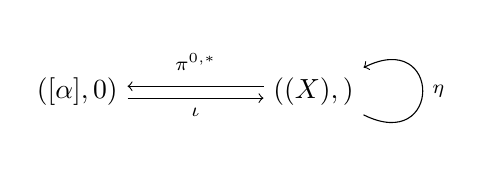
\begin{tikzpicture}[baseline=(L.base),anchor=base,->,auto,swap]
     \path node (L) {$(\fg[\alpha],0)$} ++(3,0) node (M) {$(\sG (X), \dbar)$} 
     (M.mid) +(0,.075) coordinate (raise) +(0,-.075) coordinate (lower);
     \draw (L.east |- lower) to node {$\scriptstyle \iota$} (M.west |- lower);
     \draw (M.west |- raise) to node {$\scriptstyle \pi_{\sH}^{0,*} $} (L.east |- raise);
     \draw (M.south east) ..controls +(1,-.5) and +(1,.5) .. node {$\scriptstyle \eta$} (M.north east);
  \end{tikzpicture}\end{equation*}
The map $\iota$ is the inclusion of harmonic forms. 
The operator $\eta$ is constructed from the Green's function $p(z,w) \in \Omega^{d,*}(X \times X)$ of the $\dbar$ operator on $X$, 
which satisfies 
\[
\dbar_w p(z,w) = \omega_{diag}
\]
where $\omega_{diag}$ is the volume form along the diagonal in $X \times X$. 
The homotopy $\eta$ is defined by
\[
(\eta \mu)(z) = \int_{w \in X} p(z,w) \mu(w)
\]
where $\mu$ is a $(0,*)$-form on~$X$.
This data satisfies the homotopy retraction condition
\[
\iota \circ \pi - \id_{\sG} = \dbar \eta +\eta \dbar = [\dbar,\eta],
\]
and hence ensures that we know precisely how $\sG(X)$ retracts onto its cohomology~$\fg[\alpha]$.
\end{rmk}


%Here, we view $\CC[\epsilon,\delta]$ as a cochain complex with zero differential. 


Applying Chevalley-Eilenberg chains to Equation (\ref{Lieproj}), we obtain the following quasi-isomorphism for the global sections of the untwisted Kac-Moody factorization algebra:
\beqn\label{hopfquasi3}
\begin{tikzcd}
\clieu_*(\pi_{\sH}^{0,*}) : \displaystyle \UU\sG (X) = \clieu_*(\Omega^{0,*}(X , \fg)) \ar[r,"\simeq"] &\clieu_*(\CC[\epsilon] \tensor \fg) .
\end{tikzcd}
\eeqn
Unpacking the right hand side, we have
\[
\clieu_*(\CC[\alpha] \tensor \fg) = \clieu_*(\fg \oplus \fg[-1]) = \clieu_*(\fg, \Sym (\fg^{ad})),
\] 
where $\Sym(\fg^{ad})$ is the symmetric product of the adjoint representation of $\fg$. 
By the Poincar\'{e}-Birkoff-Witt theorem, there is an isomorphism of vector spaces $\Sym(\fg) \cong U \fg$, so we can interpret this cochain complex as~$\clieu_*(\fg, U \fg^{ad})$.

Any $U(\fg)$-bimodule $M$ is automatically a module for the Lie algebra $\fg$ by the formula $x \cdot m = xm - mx$ where $x \in \fg$ and $m \in M$.
Moreover, for any such bimodule there is a quasi-isomorphism of cochain complexes 
\[
\clieu_*(\fg, M) \xto{\simeq} {\rm Hoch}_*(U\fg, M) 
\]
which is induced from the inclusion of $\fg \hookrightarrow U \fg$. 
(See, for instance, Theorem 3.3.2 of~\cite{LodayCyclic}.)
Applied to the bimodule $M = U\fg$ itself we obtain a quasi-isomorphism 
\[
\clieu_*(\fg , U\fg^{ad}) \xto{\simeq} {\rm Hoch}(U\fg).
\]
The right hand side is the Hochschild homology of $U\fg$ with values in $U\fg$ equipped with the standard bimodule structure. 
Composing with the quasi-isomorphism (\ref{hopfquasi3}) we obtain a quasi-isomorphism $\UU\sG(X) \xto{\simeq} \Hoch(U\fg)$, as desired.

We now consider the twisted case. 
Let $\theta$ be a nontrivial degree $(d+1)$ invariant polynomial on $\fg$. 
The factorization homology is then 
\[
\UU_\theta (\sG)(X) = \left(\Sym(\Omega^{0,*}(X) \tensor \fg)[K] , \dbar + \d_{CE} + K \cdot \d_\theta\right) .
\]
We wish to show that this cochain complex admits a quasi-isomorphism to $\Hoch_*(U \fg)[K]$.
The twisted complex is a $K$-linear deformation of the ordinary Lie algebra homology of $\sG(X)$. 
In particular, it does not follow that the orthogonal projection (\ref{Lieproj}) defines a quasi-isomorphism to $\Hoch_*(U \fg)[K]$.
In order to find an explicit quasi-isomorphism, we appeal to the homological perturbation lemma.
For more details on this result, see Section 2.5 of~\cite{GwThesis}. 

In the untwisted case, upon tensoring with $\CC[K]$, Remark \ref{rmk: hpl1} implies that we have a deformation retraction of cochain complexes
\begin{equation*}\tag{$\ast$}
  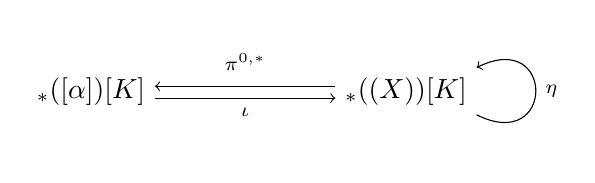
\begin{tikzpicture}[baseline=(L.base),anchor=base,->,auto,swap]
     \path node (L) {$\clieu_*(\fg[\alpha])[K]$} ++(4,0) node (M) {$\clieu_*(\sG (X))[K]$} 
     (M.mid) +(0,.075) coordinate (raise) +(0,-.075) coordinate (lower);
     \draw (L.east |- lower) to node {$\scriptstyle \iota$} (M.west |- lower);
     \draw (M.west |- raise) to node {$\scriptstyle \pi_{\sH}^{0,*} $} (L.east |- raise);
     \draw (M.south east) ..controls +(1,-.5) and +(1,.5) .. node {$\scriptstyle \eta$} (M.north east);
  \end{tikzpicture}\end{equation*}
To obtain the twisted complex, we turn on the deformation $K \, \d_\theta$ on the left-hand side. 
The homological perturbation lemma provides formulas for the resulting deformations of the projection, inclusion, and homotopy maps.
Explicitly, these formulas involve the formal inverse to the operator $\id_{\sG} - K \,\d_\theta \circ \eta$ defined by
\[
(\id_{\sG} - K \d_\theta \eta)^{-1} = \sum_{n \geq 0} \frac{K^n}{n!} (\d_\theta \circ \eta)^n  .
\] 
Note that acting on any element in the symmetric algebra~$\Sym(\Omega^{0,*}(\Omega^{0,*}(X) \tensor \fg[1])$, this formula is well-defined since only finitely many terms in the series act nontrivially.
(To see this, observe that $\d_\theta$ lowers symmetric power and $\eta$ preserves it, so any polynomial will eventually be annihilated.)

With this operator in hand, we define the maps
\begin{eqnarray*}
\widetilde{\pi}^{0,*}_{\sH} & = & \pi + K \cdot \pi \circ (\id_{\sG} - K \d_\theta \eta)^{-1} \circ \d_\theta \circ \eta, \\
\widetilde{\eta} & = & \eta + K \cdot \eta \circ (\id_{\sG} - K \d_\theta \eta)^{-1} \circ \d_\theta \circ \eta .
\end{eqnarray*}
Note that modulo $K$, these reduce to the original maps above. 
The inclusion map $\iota$ and the differential on $\clieu_*(\fg[\alpha])$ do not get deformed in our situation because the perturbed piece of the differential $\d_{\theta}$ vanishes identically on the harmonic forms. 
The homological perturbation lemma implies that the resulting diagram
\begin{equation*}\tag{$\ast$}
  \begin{tikzpicture}[baseline=(L.base),anchor=base,->,auto,swap]
     \path node (L) {$\clieu_*(\fg[\alpha])[K]$} ++(3,0) node (M) {$\UU_\theta (\sG)(X) $} 
     (M.mid) +(0,.075) coordinate (raise) +(0,-.075) coordinate (lower);
     \draw (L.east |- lower) to node {$\scriptstyle \iota$} (M.west |- lower);
     \draw (M.west |- raise) to node {$\scriptstyle \Tilde{\pi}_{\sH}^{0,*} $} (L.east |- raise);
     \draw (M.south east) ..controls +(1,-.5) and +(1,.5) .. node {$\scriptstyle \Tilde{\eta}$} (M.north east);
  \end{tikzpicture}\end{equation*}
is a deformation retraction of cochain complexes. 
With the quasi-isomorphism $\Tilde{\pi}^{0,*}_\sH$ in hand, the result of the proposition now follows from the same argument as in the untwisted case. 
\end{proof}

\subsubsection{Twisted Hochschild homology}

We deduce a consequence of this calculation for the Hochschild homology of the $A_\infty$ algebra $U(\Tilde{\fg}^\bullet_{d,\theta})$.
Let $p_{\bf q} :  \CC^d \setminus \{0\} \to X$ be the quotient map and consider the commuting diagram
\[
\xymatrix{
\CC^d \setminus \{0\} \ar[r]^-{p_{\bf q}} \ar[d]^-{r} & X \ar[d]^{\Bar{r}} \\
\RR_{>0} \ar[r]^-{\Bar{p}_{\bf q}} & S^1
}
\]
where $r$ is the radial projection map and $\Bar{r}$ is the induced map on the quotient.
The action of $\ZZ$ on $\CC^d \setminus\{0\}$ gives $\sG_{\CC^d \setminus \{0\}}$ the structure of a $\ZZ$-equivariant factorization algebra. 
In turn, $\ZZ$ acts on the pushforward factorization algebra .
We have seen that there is a locally constant subfactorization algebra on $\RR_{>0}$, equivalent as an $E_1$ (or $A_\infty$) algebra to $U(\Tilde{\fg}^\bullet_{d,\theta})$, that sits as dense subalgebra of the pushforward factorization algebra $r_* \sG_{\CC^d \setminus \{0\}}$.
The action of $\ZZ$ preserves the dense subalgebra.

This relationship induces a map at the level of global sections on the circle~$S^1$,
and it is quite interesting due to a nontrivial dependence on ${\bf q}$.
The subtlety here is that global sections coincide with the $\ZZ$-invariant global sections on $\RR$, 
i.e., the sections that are ``periodic'' with respect to the action of $\ZZ$.
For instance, the global sections of the sub-factorization algebra are {\em not} Hochschild chains of $U(\Tilde{\fg}^\bullet_{d,\theta})$, 
but a version that takes into account the monodromy around the circle.
Systematic discussions of this phenonema can be found in Section 5.5.3 of \cite{LurieHA}, Lemma 3.18 of~\cite{AFTopMan}, or Section 7.4 of~\cite{CG1}.
We denote this ${\bf q}$-twisted Hochschild homology by $\Hoch_*(U(\Tilde{\fg}^\bullet_{d,\theta}), {\bf q})$.
Concretely, it is the Hochschild homology of the $E_1$ algebra $U \Tilde{\fg}_{d,\theta}^\bullet$ with coefficients in the bimodule $U \Tilde{\fg}_{d, \theta}^\bullet$, equiped with the ordinary left module structure and right module structure determined by the automorphism corresponding to the element $1 \in \ZZ$ on the algebra.

As the locally constant factorization algebra on $\RR_{>0}$ sits inside the pushforward, 
we obtain a canonical map of global sections
\[
\Hoch_*(U(\Tilde{\fg}^\bullet_{d,\theta}), {\bf q}) \to \Bar{r}_* \UU_\alpha(\sG_X) (S^1) ,
\]
which is, in fact, a quasi-isomorphism, by our results in the preceding section. 

Now, the global sections of the pushforward factorization algebra agree with the global sections of the factorization algebra on the source space,
so we have a quasi-isomorphism
\[
\Bar{\rho}_* \UU_\alpha(\sG_X) (S^1) \simeq \UU_{\alpha} (\sG)(X) .
\]
It follows that there is a quasi-isomorphism of Hochschild homologies
\beqn\label{hoch1}
\Hoch_*(U(\Tilde{\fg}^\bullet_{d,\theta}), {\bf q}) \simeq \Hoch_* (U\fg)[K] .
\eeqn
Peculiarly, this statement is purely algebraic as the dependence on the manifold for which the Kac-Moody factorization algebra lives has dropped out.
\owen{I think this is misleading. The map depends on ${\bf q}$.}

\subsection{Character formulas by coupling to a free theory}

\def\Cl{{\rm Cl}}

We turn to a class of free field theories on Hopf manifolds that have a symmetry by the local Lie algebra $\sG_X$. 
Following Section \ref{sec: qft}, we study this situation by coupling the local Lie algebra $\sG_X$ to the free theory.
Our main result in this section, Proposition \ref{prop: twistedchar}, is an interpretation of this coupling at the {\em quantum level} as a character of~$\fg$. 

There are two main differences between the theory we consider here and the one considered in Section~\ref{sec: qft}.
First, in this section we are working on a closed $d$-fold, namely the Hopf surface $X = X_{\bf q}$. 
Although there is still a factorization algebra of observables on $X$, the main statement in this section concerns the global sections of this factorization algebra.
Since the theory actually makes sense on any complex manifold, 
our result --- which is specific to Hopf manifolds --- is an avatar of a large class of analogous results.

Second, the theory we consider here is a free theory of {\em fermions}. 
Thus, we will work with super vector spaces and super cochain complexes.
These lead to minor modifications to the approach of Section~\ref{sec: qft}, 
but yields a statement that is easiest to understand.

Before delving into the details, 
we note for physicists that we develop here a holomorphic version of the Adler-Bardeen-Jackiw anomaly,
as we are studying fermionic matter fields coupled to a background holomorphic gauge field.
(See \cite{Rabinovich} for the traditional ABJ anomaly as seen within this Costello formalism.)
A more exact comparison is with the Konishi anomaly, 
as these holomorphic theories sometimes arise as twists of supersymmetric theories.
By computing global sections on Hopf manifolds,
we recover analogues of the superconformal indices,
since a Hopf manifold has $S^1 \times S^{2d-1}$ as its underlying manifold.


\begin{rmk}
As a matter of convention, if $V$ is a super vector space, we denote by $\Pi(V)$ the super vector space obtained by reversing the parity. 
\end{rmk}

\subsubsection{The free $bc$ system}

To define the theory, we again start with a $\fg$-module $V$.
The theory is very similar in spirit to what is known as the $bc$ system in conformal field theory (which is usually considered in the context of the gauging the bosonic string). 
Hence, we borrow the terminology. 

\begin{dfn}
The {\em classical $bc$ system} valued in the super vector space $W$ on a complex manifold $X$ has space of fields
\[
\sE_{bc} (X) = \Omega^{0,*}(X , W) \oplus \Omega^{d,*}(X , W)[d-1],
\]
with the linear BRST operator given by $Q = \dbar$.
We will write fields as pairs $(c,b)$. 
There is a $(-1)$-shifted symplectic pairing is given by integration along $X$ combined with the evaluation pairing between $W$ and its dual: 
\[
\<c,b\> = \int_X \<c, b\>_{W}.
\] 
The action functional for this free theory is thus
\[
S_{bc} (c,b) = \int_X \<b , \dbar c\>_{W} .
\]
\end{dfn}

\begin{rmk}
%Note that the complex fields of this theory is a super cochain complex concentrated in completely odd super degree. 
Note that this theory is a modest variant of the definition of the higher $\beta\gamma$ system given in Section~\ref{sec: qft}. 
The only difference is that we allow for values in a super vector space $W$, as opposed to an ordinary (bosonic) one. 
When $d=1$ this theory is the usual $bc$ system (valued in $W$) from chiral conformal field theory.
\end{rmk}

Being a free theory, there is a natural BV quantization defined for any $X$.
Its definition mirrors Definition \ref{dfn: qobs} for the $\beta\gamma$ system. 
We denote the resulting factorization algebra of quantum observables by~$\Obs^\q_{bc}$. 

Before moving on to studying $\sG_X$-equivariance of this factorization algebra, we characterize the global observables of the $bc$ system with values in $W$ evaluated on Hopf manifolds. 
To state the result we introduce the following definition, whose bosonic version is familiar. 

\begin{dfn}
Let $W$ be a super vector space, and view $W \oplus W^*$ as an abelian super Lie algebra. 
Define the central extension of super Lie algebras
\[
\CC \cdot \hbar \to {\rm Heis}_\hbar (W \oplus W^*) \to W \oplus W^*
\]
arising from the $2$-cocycle defined by the natural pairing between $W$ and its dual. 
The $\hbar$-dependent {\em Weyl algebra} associated to $W$ is
\[
\Weyl_\hbar(W \oplus W^*) := U({\rm Heis}_\hbar(W \oplus W^*)) .
\]
\end{dfn}

\begin{rmk}
When $W = V$ is purely bosonic, this definition recovers the usual ($\hbar$-dependent) Weyl algebra of $V \oplus V^*$. 
When $W = \Pi(V)$ is purely fermionic, $\Weyl_\hbar(\Pi(V) \oplus \Pi(V^*))$ is the ($\hbar$-dependent) Clifford algebra of $V\oplus V^*$ associated to the natural quadratic form.  
\end{rmk} 

\begin{lem}\label{lem: hopfcliff}
Let $X$ be a Hopf manifold. 
Consider the observables of the higher $bc$ system on $X$ valued in the super vector space $W$. 
There is a natural quasi-isomorphism
\[
\Obs^\q_{bc}(X) \xto{\simeq} {\rm Hoch}_*(\Weyl_\hbar(W \oplus W^*)) .
\]
\end{lem}

\begin{proof}
The observables of any free BV theory can be modeled as the Lie algebra chains of a certain dg Lie algebra. 
(See chapter 4 of \cite{CG1}.)
For the higher $bc$ system valued in $W$, the dg Lie algebra is a (shifted) central extension of the form
\[
\CC  \,\hbar [-1] \to \Hat{\sL} \to \sL
\]
where
\[
\sL = \Omega^{d,*}(X, W^*)[d-1] \oplus \Omega^{0,*}(X, W)
\]
is an abelian dg Lie algebra and the cocycle defining the extension is
\[
\begin{array}{ccc}
\sL \times \sL & \to & \CC \, \hbar [-1]\\
 (c, b) &\mapsto& \hbar \int_X \<c, b\>_W .
\end{array}
\] 
As a cochain complex, $\Hat{\sL} = \sL \oplus \CC  \,\hbar[-1]$. 

Our proof strategy is thus to compute this Lie algebra homology by finding a small model with an obvious identification with the relevant Hochschild homology.

First, we identify this dg Lie algebra $\Hat{\sL}$ with a smaller dg Lie algebra, via Hodge theory, 
as we did in the proof of Proposition~\ref{prop: hopf}.
Thanks to  (\ref{hopfquasi}), we know how to deal with the $c$ fields,
so we turn to replacing the $b$ fields by a simpler model.

Fix a Hermitian metric and hence obtain an orthogonal projection onto the $(d,*)$-harmonic forms
\[
\pi_{\sH}^{d,*} : \left(\Omega^{d,*}(X), \dbar \right) \xto{\simeq} \sH^{d,*}_{\dbar}(X) \cong \CC\{b, b \alpha\},
\]
where $b$ has bidegree $(d,d-1)$ and $b \alpha$ has bidegree $(d,d)$.
(Note that we are using the notation of lemma~\ref{lem:tanre}.)
Observe that $\CC\{b, b \alpha\} = \CC[\alpha]b$, which is naturally isomorphic to $\CC[\alpha][-(d-1)]$,
the shift of the complex $\CC[\alpha]$ up by degree~$d-1$.

The fields with values in $W^*$ are $\Omega^{d,*}(X, W^*)[d-1] $, 
so the harmonic representative $b$ contributes a shift up by $d-1$ that cancels the shift down by $d-1$ in the definition of the fields. 
Hence we obtain a quasi-isomorphism of the $b$ fields onto their cohomology:
\[
\pi_{\sH}^{d,*} \otimes W^* [d-1]: \Omega^{d,*}(X, W^*)[d-1] \xto{\simeq} W^* \otimes \CC[\alpha],
\]
In conjunction with the map (\ref{hopfquasi}), 
we obtain a quasi-isomorphism of dg Lie algebras
\beqn
\label{hopfquasi2}
\Hat{\sL} \xto{\simeq}  \CC[\alpha] \tensor (W^* \oplus W) \oplus \CC \, \hbar [-1]. 
\eeqn
We denote the small complex on the right hand side by~$\widetilde{\sL}$.

The bracket for $\widetilde{\sL}$ is determined by the formula
\[
[1 \tensor w^* , \alpha \tensor w] = \hbar \<w^*, w\>,
\]
and the analogous formula with the roles of $w$ and $w^*$ swapped.
By directly unraveling the definitions, one finds
\[
\clieu_*(\widetilde{\sL}) = \clieu_*({\rm Heis}_\hbar(W \oplus W^*), U({\rm Heis}_\hbar(W \oplus W^*))).
\]
As we know there is a quasi-isomorphism
\[
\clieu_*(\fg, U\fg^{ad}) \xto{\simeq} \Hoch_*(U\fg)
\]
for any dg Lie algebra $\fg$,
we have a sequence of quasi-isomorphisms
\[
\clieu_*(\Hat{\sL}) \xto{\simeq} \clieu_*(\widetilde{\sL}) \xto{\simeq} \Hoch_*(U({\rm Heis}_\hbar(W \oplus W^*))).
\]
A standard result about free BV theories (see section 4.2 of \cite{CG1}) provides a quasi-isomorphism
\[
\Obs^{\q}_{bc} (X) \xto{\simeq} \clieu_*(\Hat{\sL}),
\] 
and so we have the claim, by composing all these quasi-isomorphisms.
\end{proof}

We are most interested in the case that $W = \Pi(V)$, where $V$ is an ordinary (bosonic) vector space. 
In this case, the lemma implies that there is a quasi-isomorphism
\[
\Obs^q_{bc}(X) \xto{\simeq} {\rm Hoch}_*(\Cl_\hbar(V \oplus V^*)) 
\]
where $\Cl_\hbar(V \oplus V^*)$ denotes the $\hbar$-dependent Clifford algebra. 
In this case, there is a lovely simplification of the Hochschild homology. 

If we choose a basis $\{v_i\}$ of $V$, and dual basis $\{v_i^*\}$ of $V^*$, then there is a homomorphism 
\[
\int_{Ber} : {\rm Hoch}_* (\Cl (V \oplus V^*)) \to \CC 
\]
determined by picking off the coefficient of the element $v_1 \cdots v_{\dim(V)} v_1^* \cdots v^*_{\dim(V)}$ in the Hochschild complex. 
In other words, this map is precisely the Berezin integral that projects onto the ``top fermion.'' 

It is a standard fact that the Clifford algebra is Morita trivial \cite{KasselCliff}, so that ${\rm Hoch}_*(\Cl(V \oplus V^*)) \simeq {\rm Hoch}_* (\CC) \cong \CC$.
Hence, $\int_{Ber}$ is a quasi-isomorphism. 

After inverting $\hbar$ and invoking Lemma \ref{lem: hopfcliff}, we obtain a composition of quasi-isomorphisms 
\beqn\label{hopfcliffquasi}
\Obs^\q_{bc} (X) [\hbar^{-1}] \xto{\simeq} {\rm Hoch}_*(\Cl_\hbar (V \oplus V^*)[\hbar^{-1}]) \xto{\simeq}\CC[\hbar,\hbar^{-1}] .
\eeqn
The first quasi-isomorphism is the one from Lemma~\ref{lem: hopfcliff}, and the second is Berezin integration. 
We summarize our computations as follows.

\begin{lem}
On a Hopf manifold $X_{\bf q}$, there is a natural quasi-isomorphism
\[
\Obs^\q_{bc} (X) [\hbar^{-1}] \xto{\simeq} \CC[\hbar,\hbar^{-1}]
\]
out of the quantum observables for a free fermion $bc$ system.
\end{lem}

This map encodes the ``expected value'' of a observables for this system.

\subsubsection{Quantum equivariance}

We now give our fermionic fields charge, by equipping the odd vector space $W = \Pi(V)$ with the structure of a  $\fg$-representation. 
The objective is to extract a character on the observables of the $bc$ system from the $\sG_X$-equivariant quantization. 
By the same formalism as in Section~\ref{sec: qft}, the equivariant quantization determines a quantum Noether map
\[
J_X^\q : \UU_{\Theta_X}\sG(X) [\hbar^{-1}]  \to \Obs^\q_{bc}(X) [\hbar^{-1}] ,
\]
where $\Theta_X$ is the obstruction to solving the $\sG_X$-equivariant quantization. 
\owen{Should we be using $\Cur^\q$ here rather than $\UU$?}
The explicit form of the obstruction is irrelevant in what immediately follows, but we discuss it in more detail in Section~\ref{sec: hopfobs} below. 

Combining the quasi-isomorphisms of Lemma \ref{prop: hopf} and Equation (\ref{hopfcliffquasi}), we obtain a commutative diagram
\[
\begin{tikzcd}
\UU_{\Theta_X} (\sG)(X) [\hbar^{-1}]  \ar[r, "J_X^\q"] \ar[d, "\simeq"] & \Obs^\q_{bc}(X) [\hbar^{-1}] \ar[d, "\simeq"] \\
\Hoch_*(U \fg) [\hbar^{-1}] \ar[r,dotted,"{\rm ch}_{X,V}"] & \CC[\hbar,\hbar^{-1}] .
\end{tikzcd}
\] 
The dotted map exists since the quantum Noether map preserves the projection onto the harmonic forms from which both quasi-isomorphisms are constructed.
At the level of $H^0$ we obtain the following.

\begin{prop}\label{prop: twistedchar}
The $\sG_X$-equivariant quantization of the $bc$ system on $X$ valued in the $\fg$-representation $\Pi(V)$ determines a map 
\[
{\rm ch}_{X,V} : {\rm HH}_0(U \fg)[\hbar^{-1}] = \Sym(\fg)_{\fg} [\hbar^{-1}] \to \CC[\hbar,\hbar^{-1}] .
\] 
This map is natural in the representation~$V$.
\end{prop}

As discussed earlier, a character of $\fg$ is a linear functional on ${\rm HH}_0(U \fg)$,
so we have produced an $\hbar$-dependent character from each Hopf manifold~$X$ and finite-dimensional $\fg$-representation~$V$.
Although we will not pursue an explicit formula here, 
this character ${\rm ch}_{X,V}$ varies in a beautiful way over the moduli space of Hopf manifolds,
so that one can obtain $q$-character formulas.

%Thus, $\fc(X)$ must be a 
%\[
%H^*(\Obs^{\q}_{eq}(X_{\bf q})) \xto{e^{I^\q / \hbar}} H^*_{\rm Lie}(\sG(X_{\bf q})) \tensor H^*(\Obs^\q_{bc} (X_{\bf q})) \xto{\cong} H^*(\fg, \Sym(\fg^*)) ((\hbar))
%\]

\subsubsection{A remark on the anomaly}\label{sec: hopfobs}

The $bc$ system on any manifold $X$ is {\em free}, and the anomaly $\Theta_X$ to solving the $\sG_X$-equivariant QME parametrizes the central extension of $\sG_X$ that acts on the quantum theory.

We stress that these constructions work for {\em any} complex $d$-fold $X$, 
so we can consider the higher $bc$ system on $X$ with values in the $g$-representation $\Pi(V)$. 
Furthermore, this theory is natural in the complex manifold $X$, in the sense that any holomorphic embedding of complex $d$-folds $f : X \to X'$ pulls back the $bc$ system on $X'$ to the $bc$ system on $X$. 
There is thus a ``universal'' $bc$ system on a site ${\rm Hol}_d$ of complex $d$-folds and local biholomorphisms (maps that are locally holomorphic isomorphisms).
The construction $\sG$ also determines a sheaf on this site, sending $X$ to $\Omega^{0,*}(X, \fg)$, 
and so we can consider the universal equivariant $bc$ system of $\sG$ acting on~$\sE_{bc}$. 

The anomaly $\Theta_X$ to solving the one-loop $\sG_X$-equivariant QME is encoded by a local functional of the form
\[
I_{\Theta_X}(\fc(X))=\int_X \fc(X) \wedge \Tilde{\fj}(\alpha),
\]
where $\fc(X) \in \Omega^*(X)$ and where $\Tilde{\fj}$ is a linear map of the form
\[
\Tilde{\fj} : \Sym(\sG_X[1]) \to \Omega^*(X) .
\]
Universality then puts restrictions on the differential forms that can appear in the one-loop anomaly. 

Indeed, since the anomaly $\Theta_X$ must be natural with respect to holomorphic embeddings, we see that $\fc(X)$ must be some polynomial in the Chern classes of $X$. 
Indeed, since $\Theta_X$ must also be natural with respect to holomorphic embeddings, we see that $\fc(X)$ must be some polynomial in the Chern classes of~$X$. 

For a Hopf manifold $X$, the Chern classes $c_i(X)$ vanish when $i=1,\ldots,d-1$ for degree reasons. 
Also, if we consider a local biholomorphism of the form $\CC^d \hookrightarrow X$, we see that the anomaly $\Theta_X$ must pull back to the anomaly on $\CC^d$ computed in Section~\ref{sec: qft}. 
Thus, for $X$ a Hopf manifold, the anomaly $\Theta_X$ must be proportional to a functional of the form
\[
\int_X \theta(\alpha \wedge \partial \alpha \wedge \cdots \wedge \partial \alpha)
\]
where $\theta \in \Sym^{d+1}(\fg^*)^\fg$ and $\alpha \in \sG_X$. 
In other words, we know the anomaly up to a scalar factor, which depends in some way on the representation~$V$.

To summarize, we have argued that the local class representing the extension of $\sG_X$ acting on the quantization of the $bc$ system on any Hopf manifold must be of a multiple of $\fj_X(\ch_{d+1}^\fg(V))$. 
To fully identify this class, we need machinery that we hope to develop in future work. 

\subsection{The Kac-Moody vertex algebra and compactification} 

We turn briefly to the variant of the Kac-Moody factorization algebra associated to the cocycles from Section ~\ref{sec: nekext}.
This class of cocycles is related to the ordinary Kac-Moody vertex algebra on Riemann surfaces through compactification, as we now show. 

Consider the complex manifold $X = \Sigma \times \PP^{d-1}$, 
where $\Sigma$ is a Riemann surface and $\PP^{d-1}$ is $(d-1)$-dimensional complex projective space.
Let $\omega \in \Omega^{d-1,d-1}(\PP^{d-1})$ be the natural volume form, 
which clearly satisfies the conditions of Lemma~\ref{lem: cocycle KM} and so determines a degree one cocycle $\phi_{\kappa, \omega} \in \cloc^*(\sG_{\Sigma \times \PP^{d-1}})$ after a choice of $\fg$-invariant bilinear form $\kappa : \fg \times \fg \to \CC$. 
Consider then the twisted enveloping factorization algebra of $\sG_{\Sigma \times \PP^{d-1}}$ by the cocycle~$\phi_{\kappa, \omega}$. 

Recall that if $p : X \to Y$ and $\sF$ is a factorization algebra on $X$, then the pushforward $p_* \sF$ on $Y$ is defined on opens by $p_* \sF : U \subset Y \mapsto \sF(p^{-1} U)$. 

\begin{prop}
Let $\pi : \Sigma \times \PP^{d-1} \to \Sigma$ be the projection. 
There is a quasi-isomorphism between the following two factorization algebras on $\Sigma$:
\begin{enumerate}
\item $\pi_* \UU_{\phi_{\kappa, \theta}} \left(\sG_{\Sigma \times \PP^{d-1}}\right)$, the pushforward along $\pi$ of the Kac-Moody factorization algebra on $\Sigma \times \PP^{d-1}$ of type $\phi_{\kappa,\omega}$, and
\item $\UU_{{\rm vol}(\omega) \kappa} (\sG_\Sigma)$, the Kac-Moody factorization algebra on $\Sigma$ associated to the invariant pairing ${\rm vol}(\omega) \cdot \kappa$. 
\end{enumerate}
\end{prop}

The twisted enveloping factorization on the right-hand side is the familiar Kac-Moody factorization alegbra on Riemann surfaces associated to a multiple of the pairing $\kappa$.
The twisting ${\rm vol}(\omega) \kappa$ corresponds to a cocycle of the type in the previous section 
\[
J({\rm vol}(\omega) \kappa) = {\rm vol}(\omega) \int_\Sigma \kappa(\alpha, \partial \beta)
\]
where ${\rm vol}(\omega) = \int_{\PP^{d-1}} \omega$. 

\begin{proof}
Let $U \subset \Sigma$ be an open subset. 
The factorization algebra $\pi_* \UU_{\phi_{\kappa, \theta}} \left(\sG_{\Sigma \times \PP^{d-1}}\right)$ assigns to $U$, the cochain complex
\beqn\label{KMPn}
\left(\Sym \left(\Omega^{0,*} (U \times \PP^{d-1})\right)[1] [K], \dbar + K \phi_{\kappa, \omega}|_{U \times \PP^{d-1}} \right),
\eeqn
where $\phi_{\kappa, \omega}|_{U \times \PP^{d-1}}$ is the restriction of the cocycle to the open set $U \times \PP^{d-1}$. 
Projective space is Dolbeault formal: its Dolbeault complex is quasi-isomorphic to its cohomology.
Thus, we have\footnote{Here, $\Hat{\tensor}$ is the completed projective tensor product.} 
\[
\Omega^{0,*} (U \times \PP^{d-1}) = \Omega^{0,*}(U) \Hat{\tensor} \Omega^{0,*}(\PP^{d-1}) \simeq \Omega^{0,*}(U) \Hat{\tensor} H^*(\PP^{d-1}, \sO) \cong \Omega^{0,*}(U) .
\]
Under this quasi-isomorphism, the restricted cocycle has the form
\[
\phi_{\kappa,\omega}\Big|_{U \times \PP^{d-1}} (\alpha \tensor 1, \beta \tensor 1) = \int_{U} \kappa(\alpha, \partial \beta) \int_{\PP^{n-1}} \omega 
\]
where $\alpha,\beta \in \Omega^{0,*} (U)$ and $1$ denotes the unit constant function on $\PP^{d-1}$. 
But the right hand side is precisely the value of the local functional ${\rm vol}(\omega) J_\Sigma (\kappa)$ on the open set $U \subset \Sigma$. 
Thus, the cochain complex (\ref{KMPn}) is quasi-isomorphic to 
\beqn
\left(\Sym \left(\Omega^{0,*} (U) \right)[1] [K], \dbar + K {\rm vol}(\omega) J_\Sigma (\kappa) \right) .
\eeqn
We recognize this complex as the value of the Kac-Moody factorization algebra on $\Sigma$ of type ${\rm vol}(\omega) J_\Sigma (\kappa)$.
It is immediate to see that identifications above are natural with respect to maps of opens, so that the factorization structure maps are the desired ones,
completing the proof. 
\end{proof}

Now, pick Riemann surfaces $\Sigma_1,\Sigma_2$ and let $\omega_1,\omega_2$ be their K\"{a}hler forms. 
Consider the two projections
\[
\begin{tikzcd}
& \Sigma_1 \times \Sigma_2 \arrow[dl,"\pi_1"'] \arrow[dr,"\pi_2"] & \\
\Sigma_1 & & \Sigma_2
\end{tikzcd}
\]
Consider the closed $(1,1)$-form $\omega = \pi_1^* \omega_1 + \pi_2^* \omega_2 \in \Omega^{1,1}(\Sigma_1 \times \Sigma_2)$. 
According to the proposition above, for any symmetric invariant pairing $\kappa \in \Sym^2 (\fg^*)^\fg$ this form determines a bilinear local functional
\[
\phi_{\kappa,\omega}(\alpha) = \int_{\Sigma_1 \times \Sigma_2} \omega \wedge \kappa(\alpha, \partial \alpha) 
\]
on the local Lie algebra $\sG_{\Sigma_1\times \Sigma_2}$.
A similar calculation as in the previous example implies that the pushforward factorization algebra $\pi_{i*}\UU_{\phi_{\kappa, \omega}}\sG$, $i=1,2$, is isomorphic to the Kac-Moody factorization algebra on the Riemann surface $\Sigma_i$ with level equal to the Euler characteristic $\chi(\Sigma_j)$, where $j \ne i$. 
This result was alluded to in Section 5 of Johansen \cite{JohansenKM}, 
where it is shown that there exists a copy of the Kac-Moody chiral algebra inside the operators of a twist of the $\cN=1$ supersymmetric multiplet (both the gauge and matter multiplets, in fact) on the K\"{a}hler manifold $\Sigma_1 \times \Sigma_2$. 
In Section~\ref{sec: qft} we saw how the $d = 2$ Kac-Moody factorization algebra embeds inside the operators of a free holomorphic theory on a complex surface. 
This holomorphic theory, the $\beta\gamma$ system, is the minimal twist of the $\cN=1$ chiral multiplet.
Thus, we obtain an enhancement of Johansen's result to a two-dimensional current algebra.

%\brian{relate to work of Nekrasov et al}

\section{Large $N$ limits} \label{sec: largeN}


\def\cycls{{\rm Cyc}_*}
\def\lqt{{\ell q t}}
\def\colim{{\rm colim}}
\def\sl{\mathfrak{sl}}

We take a slight detour from the main course of this paper to remark on something special that happens for the case of $\gl_N$ as $N$ goes to infinity.
The observations we make here are borrowed from unpublished work of the first author with Greg Ginot and Mahmoud Zeinalian,
but they are closely related to prior work of Costello-Li \cite{CLbcov2} and Movshev-Schwarz~\cite{} \brian{Not sure which ref you mean}.

The essential fact is the remarkable theorem of Loday-Quillen \cite{LQ} and Tsygan~\cite{Tsy},
which yields a natural map \owen{ugly notation so lets find a better one}
\[
\lqt(A) : \underset{N \to \infty}{\colim} \, \cliels(\gl_N(A)) \cong \cliels(\gl_\infty(A)) \to \Sym(\cycls(A)[1])
\]
for any dg algebra $A$ over a field $k$ of characteristic~0.
(It works even for $A_\infty$ algebras.)
Naturality here means that it works over the category of dg algebras and maps of dg algebras.
When restricted to the $\sl_\infty(k)$-invariants, we obtain a quasi-isomorphism
\[
\lqt(A) :\cliels(\gl_\infty(A))^{\sl_\infty(k)} \xto{\simeq} \Sym(\cycls(A)[1]),
\]
even when $A$ is nonunital. 
(When $A$ is unital, the $\sl_\infty(k)$-invariants are quasi-isomorphic to the full Chevalley-Eilenberg chains,
making for a very nice relationship. 
Note that it is potentially problematic to use strict invariants with a particular model for derived coinvariants of a Lie algebra,
namely Chevalley-Eilenberg chains.)

\subsection{A factorization algebra enhancement of LQT}

By taking $A$ to be the cosheaf $\Omega^{0,*}_c$ on a complex manifold $X$,
we obtain the following, whose proof is given below. 

\begin{prop}
\label{prop: cycfact}
Let $\sG l_N$ denote the local Lie algebra $\Omega^{0,*} \otimes \gl_N$.
For every $N$, there is a map of prefactorization algebras
\[
\lqt_N: \UU \sG l_N \to \Sym(\cycls(\Omega^{0,*}_c)[1])
\]
that factors through a map of prefactorization algebras
\[
\lqt: \UU \sG l_\infty \to \Sym(\cycls(\Omega^{0,*}_c)[1]).
\]
On any complex $d$-fold $X$, there is a quasi-isomorphism
\[
\lqt(X): \UU \sG l_\infty(X)^{\sl_\infty(\CC)} \to \Sym(\cycls(\Omega^{0,*}_c(X))[1]),
\]
and on closed $X$, there is a quasi-isomorphism
\[
\lqt(X): \UU \sG l_\infty(X) \to \Sym(\cycls(\Omega^{0,*}_c(X))[1]).
\]
\end{prop}

\begin{rmk}
We note that, as with the definition of the Chevalley-Eilenberg chains of a local Lie algebra,
we use here a construction of cyclic chains that plays nicely with the kind of vector spaces relevant to this situation,
namely smooth sections of vector bundles.
Where the cyclic quotient $A^{\otimes n}/C_n$ would appear for an ordinary algebra in complex vector spaces,
we take the $\Omega^{0,*}(X^n)/C_n$ and so on.
\owen{I need to check that the $\Sym$ doesn't lead to issues \dots If we must, we can ignore the quasi-isomorphism and focus on the map just to cyclic homology.}
\end{rmk}

\owen{Yes, we should do that. We could then relate to FHK again, the idea being that an extension of the cyclic jobby determines an extension of the $\gl_\infty$ jobby, which pulls back along the map to $\fg$ induced by any finite-dimensional representation. We would also obtain an interesting twist of the LQT set-up, I hope.}

This result has teeth because it is possible to compute the relevant cyclic homology.
For simplicity, consider the case where $X$ is closed, 
so that we are working with the Dolbeault complex and hence are implicitly computing the cyclic homology of the structure sheaf $\cO$ on $X$.
A standard result, see for instance Theorem 3.4.12 of \cite{LodayCyclic}, then implies that
\[
H^*(\cycls(\Omega^{0,*}(X))) \cong \bigoplus_{n \geq 0} \left( H^*(X, \Omega^n_{hol}/\partial \Omega^{n-1}_{hol}) \oplus \bigoplus_{k > 0} H^{n-2k}_{dR}(X) \right)[-n]
\]
In conjunction with the proposition, we see that the large $N$ limit of the enveloping factorization algebras $\UU \sG l_\infty$ depends primarily on the underlying topology of the complex manifold $X$, 
along with a subtle dependence on the complex geometry through the cohomology of the quotient sheaves $\Omega^n_{hol}/\partial \Omega^{n-1}_{hol}$.
In the future we hope to pursue the consequences of this observation, 
as it indicates that there is an important class of currents that can be understand through cyclic methods.
In particular, it would be interesting to relate these results to aspects of the large $N$ limits of holomorphic gauge theories.

\begin{rmk}
Loday and Procesi proved variants of the Loday-Quillen-Tsygan theorem for the Lie algebras $\mathfrak{o}_n$ and $\mathfrak{sp}_{2n}$,
in which cyclic homology of the algebra is replaced by its dihedral homology.
As nothing substantive changes in proving analogous versions of our results above, 
we do not spell out the details here.
It would be interesting to pursue the analogues of questions just raised for these Lie algebras.
\end{rmk}

\begin{proof}
The main issue is to show that $\Sym(\cycls(\Omega^{0,*}_c)[1])$ is a prefactorization algebra,
since the Loday-Quillen-Tsygan construction then implies the rest of the claim.

As $\cycls$ is a functor on the category of dg algebras, 
we see that $\cycls(\Omega^{0,*}_c)$ is a precosheaf
and hence $\cC = \Sym(\cycls(\Omega^{0,*}_c)[1])$ is also a precosheaf. 

It remains to provide the structure maps of the putative prefactorization algebra~$\cC$.
We note that for two algebras $A$ and $B$,
\[
\cycls(A) \oplus \cycls(B) \simeq \cycls(A \times B)
\] 
by \owen{find convenient reference (use the two idempotents)}.
Hence, for the cosheaf $\Omega^{0,*}_c$ on pairwise disjoint opens $U_1,\ldots, U_n$,
the isomorphism of dg algebras
\[
\Omega^{0,*}_c(U_1) \times \cdots \times \Omega^{0,*}_c(U_n) \cong \Omega^{0,*}_c(U_1 \sqcup \cdots \sqcup U_n),
\]
determines a quasi-isomorphism
\beqn
\label{eqn:cyccosheaf}
\cycls(\Omega^{0,*}_c(U_1)) \oplus \cdots \oplus \cycls(\Omega^{0,*}_c(U_n)) \xto{\simeq} \cycls(\Omega^{0,*}_c(U_1 \sqcup \cdots \sqcup U_n)).
\eeqn
Now suppose these pairwise disjoint opens $U_1,\ldots, U_n$ sit inside a larger open $V$.
We need to provide a multilinear structure map 
\beqn
\label{eqn: desiredmap}
\cC(U_1) \times \cdots \times \cC(U_n) \to \cC(V)
\eeqn
to describe $\cC$ as a prefactorization algebra.
The inclusion $U_1 \sqcup \cdots \sqcup U_n \hookrightarrow V$ provides a map
\[
\cycls(\Omega^{0,*}_c(U_1 \sqcup \cdots \sqcup U_n)) \to \cycls(V),
\]
via the precosheaf $\cycls(\Omega^{0,*}_c)$,
and so applying $\Sym$ gives us
\beqn
\label{eqn:map2}
\cC(U_1 \sqcup \cdots \sqcup U_n) \to \cC(V).
\eeqn
Likewise, applying $\Sym$ to map \eqref{eqn:cyccosheaf} provides
\[
\cC(U_1) \times \cdots \times \cC(U_n) \to \cC(U_1 \sqcup \cdots \sqcup U_n).
\]
We thus obtain the desired map \eqref{eqn: desiredmap} as a composite.
This construction is automatically associative for nested inclusions of pairwise disjoint opens,
and so $\cC$ is a prefactorization algebra.
\end{proof}

\subsection{Local cyclic cohomology}

The concept of a local Lie algebra is the starting point for our definition of the factorization enveloping algebra and current algebra. 
We obtain a similar notion by replacing a (dg) Lie algebra with a (dg) associative algebra.

\begin{dfn}
A {\em local dg algebra} on a smooth manifold $X$ is:
\begin{enumerate}
\item[(i)] a $\ZZ$-graded vector bundle $A$ on $X$ of finite total rank, whose sheaf of sections we denote $\sA^{sh}$;
\item[(ii)] a degree one differential operator $\d : \sA^{sh} \to \sA^{sh}$;
\item[(iii)] a degree zero bidifferential operator $\cdot : \sA^{sh} \times \sA^{sh} \to \sA^{sh}$
\end{enumerate}
such that the collection $(\sA^{sh}, \d, \cdot)$ has the structure of a sheaf of dg associative algebras.
\end{dfn}

As usual, we abusively refer to a local algebra $(\sA^{sh}, \d, \cdot)$ simply by $\sA$.
On a complex manifold, the basic example for us of a local algebra is the Dolbeault complex $\Omega^{0,*}_X$. 
Of course, this is a commutative local algebra. 
For a noncommutative example, one can take the sheaf of holomorphic differential operators, and take its Dolbeault resolution. 

There is a forgetful functor from local algebras to local Lie algebras. 
In particular, given any local algebra $\sA$ and local Lie algebra $\sL$ we obtain a new local Lie algebra $\sL \tensor \sA$.
The underlying vector bundle is simply $L \tensor A$. 

We now move on to discuss twisted versions of the relationship between cyclic homology and the Kac-Moody factorization algebra for $\fgl_\infty$. 
For this, we need a local notion of a cyclic cocycle. 

For local algebras, there is an appropriate notion of cohomology respecting the locality, analogous to local Lie algebra cohomology. 
To define it, first consider the underlying $\ZZ$-graded vector bundle $A$ of a local algebra. 
The $\infty$-jet bundle of $A$ is denoted by $JA$.
Then, $JA$ defines an associative dg algebra in the category of $D_X$-modules. 
Further, its Hochschild complex $\Hoch^*(JA)$ also has the structure of a $D_X$-module. 
We use this observation in the definition below. 

\def\Hoch{{\rm Hoch}}
\def\Hochloc{{\rm Hoch}_{\rm loc}}
\def\Cyc{{\rm Cyc}}
\def\Cycloc{{\rm Cyc}_{\rm loc}}

\begin{dfn}\label{dfn: hochloc}
The {\em local Hochschild cohomology complex}  of a local algebra $\sA$ on $X$ is 
\[
\Hochloc^*(\sA) = \Omega^*_X[2d] \tensor_{D_X} \Hoch^*_{red} (JA) .
\] 
This sheaf of cochain complexes has global sections that we denote by $\Hochloc^*(\sA(X))$.
\end{dfn}

Just as in local Lie algebra cohomology, we can concretely understand an element in $\Hochloc^*(\sA)$ as follows.
It is a polynomial functional on $\sA$ that is a finite sum of functionals of the form
\[
\alpha_1 \tensor \cdots \alpha_k \mapsto \int_X \omega_X \wedge D_1(\alpha_1) \cdots D_k(\alpha_k)
\]
where $D_i$ is a differential operator from $\sA$ to $C^\infty(X)$ and $\omega_X$ is a volume form on $X$. 

There is also a cyclic version of the Hochschild cohomology. 
The dg $D$-module of reduced Hochschild cochains on $JA$ is of the form
\[
\Hoch_{red}^* (JA) = \prod_{n > 0} {\rm Hom}_{C^\infty_X} (JA^{\tensor n}, C^\infty_X) .
\]
For each $n$, there is an action of the cyclic group $C_n$ on $JA^{\tensor n}$. 
There is a resulting action of the group $S_n$ on each graded piece of the reduced Hochschild complex $\Hoch_{red}^* (JA)$.
We obtain the termwise quotient $D$-module by
\[
\Cyc_{red}^* (JA) = \prod_{n > 0} {\rm Hom}_{C^\infty_X} (JA^{\tensor n}, C^\infty_X) / C_n .
\]
The Hochschild differential restricts to this subspace to yield a dg $D$-module. 

We repeat Definition \ref{dfn: hochloc} for the cyclic version of local cohomology of a local algebra $\sA$. 

\begin{dfn}\label{dfn: cycloc}
The {\em local cyclic cohomology complex}  of a local algebra $\sA$ on $X$ is 
\[
\Cycloc^*(\sA) = \Omega^*_X[2d] \tensor_{D_X} \Cyc^*_{red} (JA) .
\] 
This sheaf of cochain complexes has global sections that we denote by $\Cycloc^*(\sA(X))$.
\end{dfn}

As we've mentioned, the most relevant local algebra for us will be the Dolbeault complex $\Omega^{0,*}_X$ defined on an arbitrary complex manifold. 
For this local Lie algebra, there is a natural degree zero cocycle in local cyclic cohomology.
The reader may observe its very similar form to its counterpart in local Lie algebra cohomology introduced in Section \ref{sec: localcocycle}. 

\begin{lem}
\label{lem: univ}
Fix a complex dimension $d$. 
The functional $\Theta^\infty_d$ on $\Omega^{0,*}$ defined by
\[
\Theta^\infty_d : \alpha_0 \tensor \cdots \tensor \alpha_d \mapsto \alpha_0 \wedge \partial \alpha_1 \cdots \wedge \partial \alpha_d
\]
is a degree zero cocycle in $\Cycloc^*(\Omega^{0,*})$. 
\end{lem}
\begin{proof}
The proof is very similar to that of Proposition \ref{prop j map}. 
Note that the differential on local cochains consists of two terms: the $\dbar$ operator and the ordinary Hochschild differential. 
It follows from graded commutativity of the wedge product that the cochain is cyclic and closed for the Hochschild differential. 
To see that it is closed for the other piece of the differential, observe that
\[
\dbar \Theta^\infty_d(\alpha_0,\cdots,\alpha_d) = \Theta^\infty_d(\dbar \alpha_0, \alpha_1,\ldots,\alpha_d) \pm \Theta_d^\infty(\alpha_0, \dbar \alpha_1,\ldots \alpha_d) \pm \cdots \pm \Theta_d^\infty(\alpha_0, \alpha_1,\ldots \dbar \alpha_d) .
\]
The right hand side is the cocycle $\Theta_d^\infty$ evaluated on the derivation $\dbar$ applied to the element $\alpha_0 \tensor \cdots \tensor \alpha_d$. 
The left hand side is a total derivative, hence vanishes in the local cochain complex. 
\end{proof}

We refer to $\Theta^\infty_d$ as a `universal' cocycle in the sense that it only depends on the complex dimension and not on any Lie algebraic data. 
It determines a ``twist" of the prefactorization algebra 
\[
\Sym(\cycls(\Omega^{0,*}_c)[1])
\]
of Proposition \ref{prop: cycfact} by a $\CC[K]$-linear deformation of the differential $\dbar + \d_{\rm Hoch}$ to
\[
\dbar + \d_{\rm Hoch} + K \cdot \Theta^\infty_d ,
\] 
where $K$ is some formal variable. 

We turn to the relationship between cyclic cocycles for a local algebra $\sA$ and cocycles for the local Lie algebras $\gl_N \tensor \sA$ and $\gl_\infty \tensor \sA$.

\begin{prop}
\label{prop: cycloc}
Let $\sA$ be a local algebra.
For every $N > 0$, there is a map of sheaves
\[
\lqt_N^* : \Cycloc^*(\sA)[-1] \to \cloc^*(\gl_N \tensor \sA) 
\] 
that factors through a map of sheaves
\[
\lqt^* : \Cycloc^*(\sA)[-1] \to \cloc^*(\gl_\infty \tensor \sA) = \lim_{N \to \infty} \cloc^*(\gl_\infty \tensor \sA)  .
\]
%\[
%\lqt : \Hat{\Sym}^{>0} \left(\Cycloc^*(\sA)[-1]\right) \to \cloc^*(\gl_\infty \tensor \sA)  
%\]
\end{prop}

\brian{Check my shifts.}
%\brian{We could state their result about PV fields using HKR, but I don't know if that buys us anything too amazing at this point.}

\begin{rmk}
A version of this result has been proved in \cite{CL1} for the case $\sA = \Omega^{0,*}(X)$ where $X$ is a Calabi-Yau manifold.
They interpret local cocycles for $\Omega^{0,*}(X) \tensor \fgl_\infty$ as the space of admissible deformations for holomorphic Chern-Simons on $X$. 
They identify the cyclic side with the space of fields for Kodaira-Spencer gravity \cite{BCOV} on $X$.
\end{rmk}

Proposition \ref{prop: cycloc} gives us a way to construct degree one cocycles for the local Lie algebra $\fgl_N \tensor \Omega^{0,*} = \sG l_{N}$. 
Indeed, the inclusion $\fgl_N \hookrightarrow \fgl_\infty$ induces a map of cochain complexes 
\[
\cloc^*(\gl_\infty \tensor \sA) \to \cloc^*(\gl_N \tensor \sA)
\]
by pull back. 
The universal degree zero cocycle $\Theta_d^\infty \in \Cycloc^*(\Omega^{0,*})$ from Lemma \ref{lem: univ} thus determines a degree one cocycle 
\[
\lqt^*_N(\Theta_d^\infty) \in \cloc^*(\sG l_N)
\]
for each $N > 0$. 

In fact, this procedure produces the particular class of cocycles for $\sG l_{N}$ that we have already met. 
Note that for each $N$ and $k$, the functional $\theta_{k,N} : A \mapsto {\rm tr}_{\fgl_N} (A^k)$ defines a homogenous degree $k$ polynomial on $\fgl_N$. 
In this way, we obtain $\fgl_N$-invariant elements
\[
\theta_{k,N} \in \Sym^{k}(\fgl_N^*)^{\fgl_N} .
\]

\begin{lem}
For every $N$, the image of $\Theta_d^\infty$ under the Loday-Quillen-Tsygan map $\lqt_N^*(\Theta_d^\infty)$ is equal to the cocycle
\[
\fj(\theta_{d+1, N}) \in \cloc^*(\sG l_N)
\]
where $\fj$ is as in Definition \ref{dfn: j}
\end{lem}

\begin{proof}
Let $A$ be any algebra and consider the Lie algebra $\fgl_N(A)$ and the limit $\gl_\infty(A) = {\rm colim} \; \fgl (A)$. 
At the level of homology, the ordinary Loday-Quillen-Tsygan map is of the form
\[
\begin{array}{ccc}
H_{n+1}^{\rm Lie}(\fgl_N(A)) & \to & HC_{n}(A) \\
X_0 \wedge \cdots \wedge X_n & \mapsto & \sum_{\sigma \in S_n} (-1)^{\sigma} {\rm tr} \left(X_0 \tensor X_{\sigma(1)} \tensor\cdots \tensor X_{\sigma(n)} \right) 
\end{array}
\] 
which induces a dual map in cohomology $HC^n(A) \to H^{n+1}_{\rm Lie}(\fgl_N(A))$. 
Here, ${\rm tr}$ denotes the generalized trace map
\[
{\rm tr} : {\rm Mat}_N(A)^{\tensor(n+1)} \to A^{\tensor (n+1)} 
\]
which maps a $(n+1)$-tuple $A_0\tensor \cdots \tensor A_d$ to 
\[
\sum_{i_0,\ldots,i_n} (A_0)_{i_0 i_1} \tensor (A_1)_{i_1i_2} \tensor \cdots \tensor (A_n)_{i_n i_0}
\]
where $(A_k)_{ij} \in A$ denotes the $ij$ matrix entry.

The map on local functionals is essentially this ordinary (dual) Loday-Quillen-Tsygan map applied to the $\infty$-jets of the commutative algebra $\Omega^{0,*}$. 
Since $\Omega^{0,*}$ is commutative, the generalized trace is simply the trace of the product.
%so that for any $\varphi \in \Cycloc^*(\Omega^{0,*})$ of homogenous degree $n$, one has
%\[
%\lqt_N^*(\varphi) (\alpha_0,\ldots,\alpha_n) = {\rm tr}_{\fgl_N}(\alpha_0 \wedge \cdots \wedge \alpha_d) . 
%\]
%\[
%\begin{array}{ccccc}
%{\rm tr} & : & {\rm Mat}_N(\Omega^{0,*})^{\tensor (n+1)} & \to & (\Omega^{0,*})^{\tensor (n+1)} \\
%& & \alpha_0 \tensor \cdots \alpha_d
%\end{array}
%\]
We can thus read off the image of $\Theta^\infty_d$ under the $\ell q t_N^*$ as the local Lie algebra cocycle

\begin{align*}
\ell q t_N^*(\Theta_d^\infty)\left(\alpha_0, \cdots, \alpha_d) = {\rm tr}_{\fgl_N}(\alpha_0 \wedge \partial \alpha_1 \cdots \wedge \partial \alpha_d\right)
\end{align*}
which is precisely $\fj(\theta_{d+1,N})$. 
\end{proof}

As an immediate corollary, we obtain a twisted version of Proposition \ref{prop: cycfact}.
Indeed, the compatibility of the cyclic cocycle $\Theta^\infty_d$ and $\fj(\theta_{d+1,N})$ implies that there is a map of prefactorization algebras
\[
\UU_{\fj(\theta_{d+1,N})} (\gl_N) \to \left(\Sym(\cycls(\Omega^{0,*}_c)[1])[K], \dbar + \d_{\rm Hoch} + K \cdot \Theta^\infty_d \right) .
\]
%\[
%\UU_{\fj(\theta_{d+1,\infty})} (\gl_\infty) \to \left(\Sym(\cycls(\Omega^{0,*}_c)[1])[K], \dbar + \d_{\rm Hoch} + K \cdot \Theta^\infty_d \right)
%\]

\brian{There is a statement about the hol trans invariant cyclic cochains.
Namely that it's one dimensional generated by the higher residue.
This is complementary to FHK and is compatible with out calculation in the appendix under the LQT map. 
Should I include a remark about this?
}

\subsection{A noncommutative example}

Suppose $(X,\omega)$ is a holomorphic symplectic manifold, and let $\{-,-\}_\omega$ be the Poisson bracket on holomorphic functions. 
This bracket extends to one on the Dolbeault complex $\Omega^{0,*}(X)$. 
For any $N$, we then obtain the dg Lie algebra
\[
\sL(X,\omega) = \left(\Omega^{0,*}(X) \tensor \fgl_N , \{-,-\}_\omega\right) .
\]
This is clearly a local Lie algebra. 

Now, suppose $\star_\epsilon$ is a formal holomorphic deformation quantization of $(X,\omega)$. 
This associative product on $\sO^{hol}(X)[[\epsilon]]$ extends to one on the Dolbeault complex giving
\[
\sA(X,\star_{\epsilon}) = (\Omega^{0,*}(X)[[\epsilon]], \star_{\epsilon})
\]
the structure of a dg associative algebra. 
In fact, it is a local algebra. 
Furthermore, for each $N$ the dg Lie algebra 
\[
\sA(X, \star_{\epsilon}) \tensor \fgl_N
\]
is a deformation of the local Lie algebra $\sL(X,\omega)$. 


\appendix

\section{Computing the deformation complex}\label{sec: hol trans}

In this appendix we prove Proposition~\ref{prop: trans j}. 
That is, we compute the holomorphically translation invariant component of $H_{\rm loc}(\sG_d)$, 
the Lie algebra cohomology of the local Lie algebra $\sG_d = \Omega^{0,*}_c \tensor \fg$ on~$\CC^d$. 

We have already discussed the local cohomology cochain complex $\cloc^*(\sG_d)$ in Section~\ref{sec:cloc}.
To pick out the subcomplex of holomorphically translation invariant elements,
we introduce yet another dg Lie algebra $\CC^{d}_{\rm hol}$ whose invariants are precisely this subcomplex.

\begin{dfn}
Let $\CC^{d}_{\rm hol} = \CC^{2d} \oplus \CC^d[1]$ be generated by the partial derivatives $\partial/\partial z_i$ and $\partial/\partial \zbar_i$ in degree 0 and by elements $\{\Bar{\eta}_i\}_{i=1}^d$ in degree $-1$.
Equip it with a trivial bracket and with a differential that $\eta_i$ to $\frac{\partial}{\partial \zbar_i}$.
\end{dfn}

There is a canonical inclusion of dg Lie algebras
\[
\CC\{\partial / \partial z_1, \ldots, \partial / \partial z_d\} \hookrightarrow \CC^{d}_{\rm hol}
\]
so that any representation ``forgets'' down to an action of holomorphic infinitesimal translations.
But a dg representation of this abelian dg Lie algebra has an action of all the partial derivatives,
but where the actions of the $\partial/\partial \zbar_i$ are trivial homotopically.
In this sense $\CC^{d}_{\rm hol}$ encodes the idea of infinitesimal translations that are purely holomorphic up to homotopy.

Directly from these definitions one can verify the following.

\begin{lem}
The canonical inclusion of enveloping algebras
\[
\CC[\partial / \partial z_1, \ldots, \partial / \partial z_d] \hookrightarrow U(\CC^{d}_{\rm hol})
\]
that is a quasi-isomorphism.
\end{lem}

In other words, $U(\CC^{d}_{\rm hol})$ is quasi-isomorphic to the algebra of constant coefficient holomorphic differential operators on~$\CC^d$. 

We now turn to the main objects of interest here.

\begin{dfn}
Let $\cloc^*(\sG_d)^{\CC^d_{\rm hol}}$ denote the subcomplex in $\cloc^*(\sG_d)$ consisting of elements strictly invariant under $\CC^d_{\rm hol}$.
Let
\[
\cloc^*(\sG_d)^{U(d) \ltimes \CC^d_{\rm hol}}
\]
denote the subcomplex of elements that are invariant under both translation by $\CC^d_{\rm hol}$ and rotation by the unitary group~$U(d)$.
\owen{Check which semi-direct product.}
\end{dfn}

We are interested in the map $\fj$, from Section~\ref{sec: hol trans main}, for the affine space $\CC^d$.
We will use this map to completely characterize the degree one $U(d)$-invariant, holomorphically translation invariant local functionals on~$\sG_d$. 

The degree one result will follow from a stronger, general result on the cochain level.
To formulate it, we introduce some notation.

Let $\cL$ denote an arbitrary dg Lie algebra. 
Interpret the dg commutative algebra given by the Chevalley-Eilenberg cochains $\clie^*(\cL)$ as functions on a formal moduli space~$B \cL$:
\[
\sO(B \cL) = \clie^*(\cL) .
\]
In the same line of thought, define the $k$-forms on $B\cL$~by
\[
\Omega^k(B \cL) := \clie^*(\cL ; \Sym^k(\cL^\vee [-1])) .
\]
Here, $\cL^\vee$ denotes the coadjoint representation of~$\cL$. 
Furthermore, let $\partial : \Omega^{k}(B\cL) \to \Omega^{k+1}(B\cL)$ denote the de Rham operator for $B\cL$. 
The space of {\em closed} $k$-forms is defined by the totalization of the double complex
\[
\Omega^{k}_{cl}(B \cL) = {\rm Tot}\left( \Omega^k(B\cL) \xto{\partial} \Omega^{k+1}(B \cL)[-1] \to \cdots \right).
\]
Note that there is a canonical truncation map $\Omega^{k}_{cl}(B \cL) \to \Omega^{k}(B \cL)$ that provides the ``underlying'' $k$-form of any closed $k$-form.

\begin{eg}
A simple example gives evidence that this interpretation is not so far-fetched.
Consider the case $\cL = \CC^n [-1]$, a purely abelian Lie algebra.
Then
\[
\sO(B \cL) = \clie^*(\cL) = \CC[[t_1,\ldots,t_n]]
\]
with generators $t_i$ in degree 0.
(These generators are the coordinates on the formal $n$-disk.)
Similarly, the de Rham forms are
\begin{align*}
\Omega^k(B \cL) 
&= \sO(B \cL)  \otimes \Lambda^k(\cL^\vee) \\
 &=\CC[[t_1,\ldots, t_n]] \tensor \Lambda^k[\d t_1, \cdots, \d t_n],
\end{align*}
where we use $\d t_i$ to denote a basis for the coadjoint representation~$\cL^\vee$.
(We use $\Lambda^k$ denote the $k$th exterior power of the vector space spanned by those generators.)
Everything is in cohomological degree zero.
Manifestly everything agrees with the usual constructions of algebraic de Rham forms.
\end{eg}

Before stating the main result of this appendix, we note that there is a natural enhancement of the cochain map
\[
\fj : \Sym^{d+1} (\fg^*)^{\fg} [-1] \to \cloc^*(\sG_d)
\]
from Section \ref{sec: hol trans main} to a cochain map
\beqn\label{fj1}
\fj : \Omega^{d+1}_{cl} (B \fg) [d] \to \cloc^*(\sG_d)  
\eeqn
that we now describe. 
\owen{What do you mean here by "closed" forms? What you wrote below suggests you had something strict in mind (the actual de Rham closed forms) ... a lot of what's below seems like a detour. I'm not sure we need all this discussion to say the key fact.}

\owen{I commented out much of the description below, which seemed irrelevant to the construction.}

%Consider the map of cochain complexes
%\[
%\CC[1] \to \Omega^*(B \fg)
%\]
%where we are viewing $\CC$ as sitting inside $\Omega^0(B \fg) = \clie^*(\fg)$ as the constant functions. 
%The totalization of this map of complexes is acyclic. 
%
%Let $\Omega^{\leq d}(B \fg)$ denote the cokernel of the injective map of cochain complexes
%\[
%\Omega^{d+1}_{cl} (B \fg) [-d-1] \hookrightarrow {\rm Tot}\left(\CC[1] \to \Omega^*(B \fg)\right)  .
%\]
%Notice, by acyclicity of the target of this map, the de Rham differential induces a quasi-isomorphism
%\[
%\partial : \Omega^{\leq d}(B \fg) \xto{\simeq} \Omega^{d+1}_{cl}(B \fg) .
%\] 
%Notice that on the formal disk $\fg = \CC^n[-1]$, this quasi-ismorphism implies the standard fact that every closed $(d+1)$-form can be written as the de Rham differential applied to a $d$-form. 

\owen{The behavior of $\widetilde{\fj}$ on $d+k$-forms is not described. Is that $k < d$ a typo? I }

The map we want (\ref{fj1}) is induced from a map defined on this quasi-isomorphic complex
\[
\widetilde{\fj} : \Omega^{\leq d}(B \fg) \to \cloc^*(\sG_d) .
\] 
This map is zero on the graded pieces $\Omega^k (B \fg)$ for $k < d$. 
Given a $d$-form, $\eta \in \Omega^d(B \fg)$ we define the local functional $\widetilde{\fj}(\eta)$ by 
\[
\widetilde{\fj} (\eta) (\alpha) = \eta (\partial \alpha \wedge \cdots \wedge \partial \alpha) (\alpha) .
\]
Here, $\eta (\partial \alpha \wedge \cdots \partial \alpha)$ denotes the pairing of $\Wedge^d \fg^\vee$ with the $d$th exterior power of $\Omega^{1,*}(X) \tensor \fg$ which results in an element of $\Omega^{d,*} \tensor \clie^*(\fg)$. 
\owen{I'm not sure this makes sense as written: you're ignoring all the stuff that comes from the $\clie^*(\fg)$ direction. Why should $\eta$ have the form you're asserting?}
We then use the remaining Lie algebra factors of $\eta$ to pair with $\Omega^{0,*}(X) \tensor \fg$. 
The result is an element in $\Omega^{d,*}(X)$, and by our usual conventions, our local functional only remembers the top component $\Omega^{d,d}(X)$. 
\owen{Do you mean we integrate over $X$ or that we just drop all other degrees?}

Note that if the $d$-form $\eta$ is exact, given by the de Rham differential of a $(d-1)$-form, then the functional $\widetilde{\eta}$ is identically zero since we quotient out by total derivatives in our definition of local functionals. 
\owen{No, we don't. We work with the de Rham complex of the Lagrangian densities.}
Thus, we see that $\widetilde{\fj}$ descends, along the de Rham differential $\partial$, to a cochain map (\ref{fj1}) as desired. 


\owen{We should explain what it is, at least briefly.}

\begin{prop}\label{prop: local def}
The map $\fj$ factors through the subcomplex of invariants under rotation and holomorphic translation:
\beqn
\fj : \Omega^{d+1}_{cl}(B \fg) [d] \to \cloc^*(\sG_d)^{U(d) \ltimes \CC^d_{\rm hol}}.
\eeqn
In particular, if $\fg$ is an ordinary Lie algebra (i.e., concentrated in degree zero), then we obtain an isomorphism
\[
H^1(\fj) : \Sym^{d+1}(\fg^\vee)^\fg \xto{\cong} H^1  \left(\cloc^*(\sG_d)\right)^{U(d) \ltimes \CC^d_{\rm hol}}.
\] 
\end{prop}

Note that this result contains Proposition~\ref{prop: trans j}.

\owen{As it was written, I'm confused about the proof of this proposition. We need to discuss.}

\owen{Why do we take the detour through $\CC^{d}_{\rm hol}$ if we just end up working with the invariants for $\CC\{\partial/\partial z_i\}$?}

\brian{It's in formula \ref{holtransinvt}. 
I want to say that were taking the invariants of the actual space of local functionals with respect to some (dg) Lie algebra.  
Of course, in holomorphic situations its natural to throw away anti-holomorphic factors, but this dg Lie algebra allows us to do that in a systematic way.}

In brief, the proof involves two central ideas.
The first is that the translation-invariant local functionals ought to be built from translation-invariant differential operators and translation-invariant measures,
and such functionals are thus pinned down by their behavior at one point.
The second is that rotation invariance then drastically cuts down the remaining possibilities.
Indeed, as the proposition indicates, the only freedom is concentrated in the dependence on the Lie algebra $\fg$ and not on the spatial directions along~$\CC^d$.

\begin{lem}
The subcomplex $\cloc^*(\sG_d)^{\CC^d}$ of elements invariant under translation along $\CC^d$ is isomorphic to 
\[
\cred^*(\fg[[z_1,\ldots,z_n, \zbar_1,\ldots, \zbar_n, \d\zbar_1,\ldots, \d\zbar_n]]),
\]
the reduced Lie algebra cochains on the dg Lie algebra $\fg[[z_1,\ldots,z_n, \zbar_1,\ldots, \zbar_n, \d\zbar_1,\ldots, \d\zbar_n]]$ whose differential is~$\dbar$.
\end{lem}

That dg Lie algebra is Dolbeault forms on the formal $d$-dimensional disk with values in~$\fg$.

\begin{proof}
Here we are just noting a simple fact: 
our bundle $\fg \times \CC^d \to \CC^d$ is trivial,
and hence the jet bundle inherits a trivialization.
The trivialization is explicitly given by using the linear coordinate system arising from identifying the manifold with the vector space $\CC^d$;
it gives a natural basis for differential operators and hence for jets.
Translation-invariant sections are thus determined by their value at a single point,
which we can take to be the origin.
The fiber of the jet bundle at the origin can be seen as Dolbeault forms on the formal $d$-dimensional disk with values in $\fg$.
As $\cloc^*$ is a version of reduced Lie algebra cochains, we obtain the claim.
\end{proof}

We would now like to trivialize homotopically the action of the antiholomorphic derivatives.
On the formal $d$-dimensional disk, there is a natural trivialization (by contraction with the vector fields $\partial_{\zbar_i}$),
which also makes sense on $\CC^d$ globally.
\owen{I'm writing quickly ... need to check that. It now doesn't sound quite right.}
The strict invariants for the extended Lie algebra $\CC^d_{\rm hol}$ are thus expressions that have no dependence on the antiholomorphic coordinates~$\zbar_i$.

\begin{lem}
The $\CC^d_{\rm hol}$-invariant subcomplex $\cloc^*(\sG_d)^{\CC^d_{\rm hol}}$ is isomorphic to 
\[
\cred^*(\fg[[z_1,\ldots,z_n]]),
\]
the reduced Lie algebra cochains of the Lie algebra~$\fg[[z_1,\ldots,z_n]]$.
\end{lem}

In practice the proof involves a number of quasi-isomorphisms and a spectral sequence,
so it is convenient to isolate some of these results as lemmas.
We begin by describing the situation on a formal $d$-dimensional disk with formal coordinates $z_1,\ldots, z_d$.
In this case $\sG_d$ has the form $\fg[[z_1,\ldots,z_n]]$, and 
\beqn
\cred^*(\fg[[z_1,\ldots,z_n]]) = \left(\Sym^{\geq 1} \left(\fg^\vee [z_1^\vee,\ldots,z_d^\vee][-1] \right), \d_{\fg}\right),
\eeqn
where $z_i^\vee$ denotes the dual variable to $z_i$. 
A cocycle in this complex encodes the jet of a Lagrangian on the formal disk.
To get the jet of a Lagrangian density, we pair such a cocycle with a top form, namely~$\d^d z$,
but we want to consider such Lagrangian densities up to total derivatives,
i.e., modulo integration by parts.
This relation is cleanly encoded as the relative (derived) tensor product
\[
\CC \, \d^d z \tensor^\LL_{\CC\left[\frac{\partial}{\partial z_i}\right]} \cred^*(\fg[[z_1,\ldots,z_d]]).
\]
\owen{Should we bother to justify this?}
There is then a simple answer for which such elements are $U(d)$-invariant.

\begin{lem}
The $U(d)$-invariant subcomplex 
\[
\left( \CC \, \d^d z \tensor_{\CC\left[\frac{\partial}{\partial z_i}\right]} \cred^*(\fg[[z_1,\ldots,z_d]]) \right)^{U(d)}
\]
is canonically isomorphic to the reduced de Rham forms
\[
\Omega^\sharp_{\rm red}(B\fg) = \sO_{red}(B \fg) \oplus \Omega^{1} (B \fg)[-1] \oplus \cdots \oplus \Omega^{d}(B \fg)[-d]. 
\]
\end{lem}

Here we mean that there is no de Rham differential, 
but the $k$-forms are put in their ``usual'' place 
(i.e., in our motivating example, the $k$-forms would sit in degree $k$).
By $\sO_{red}(B \fg)$ we mean that we quotient out the copy $\Sym^0(\fg^\vee)$ of the constants from~$\clie^*(\fg)$.

\begin{proof}[Proof of lemma]
Sitting inside of $U(d)$, there is a copy of $U(1)$ as multiples of the identity.
\owen{Note that I use $U(1)$ for the group, rather than $S^1$, which is most obviously a space.} 
This group equips the complex with a weight grading, as follows.
The group $U(d)$ acts in the defining way on $\CC^d$,
so each $z_i$ has weight $1$ while both $z_i^\vee$ and $\frac{\partial}{\partial z_i}$ have weight~$-1$. 
The volume element $\d^d z$ has weight $d$.
It follows that in order to have total weight zero, a monomial in these terms must have its total number of $\frac{\partial}{\partial z_i}$ and $z_i^\vee$ add up to $d$.
Thus, as a graded vector space, the invariant subcomplex decomposes
\beqn
\bigoplus_{k \geq 1} \Sym^k(\CC^d[1]) \tensor \left(\bigoplus_{i \leq d-k} \Sym^{i} \left(\fg^\vee [z_1^\vee,\ldots,z_d^\vee][-1] \right) \right) \d^d z [d] .
\eeqn
It follows from Schur-Weyl that the space of $U(d)$ invariants of the $d$th tensor power of the fundamental representation $\CC^d$ is one-dimensional, spanned by the top exterior power. 
Thus, when we pass to the $U(d)$-invariants, only the unique totally antisymmetric tensor involving $\frac{\partial}{\partial z_i}$ and $z_i^\vee$ survives. 
Thus, for each $k$, we have
\begin{align}
\label{U(d) invariants}
\left(\Sym^k(\CC^d[1]) \tensor \right. & \left. \left(\bigoplus_{i \leq d-k} \Sym^{i} \left(\fg^\vee [z_1^\vee,\ldots,z_d^\vee][-1] \right) \right) \d^d z\right) \cong \\ & \wedge^{k}\left(\frac{\partial}{\partial z_i}\right) \wedge \wedge^{d-k}\left(z_i^\vee\right) \clie^*\left(\fg , \Sym^{d-k}(\fg^\vee)\right) \d^d z .
\end{align}
Here, $\wedge^{k}\left(\frac{\partial}{\partial z_i}\right) \wedge \wedge^{d-k}\left(z_i^\vee\right)$ is just a copy of the determinant $U(d)$-representation, but we'd like to keep track of the appearances of the partial derivatives and $z_i^\vee$. 
Note that for degree reasons, we must have $k \leq d$. 
When $k = 0$ this complex is the (shifted) space of functions modulo constants on the formal moduli space $B\fg$, $\sO_{red}(B\fg)[d]$. 
When $k \geq 1$ this the (shifted) space of $k$-forms on the formal moduli space $B\fg$, which we write as $\Omega^{k}(B \fg)[d+k]$.
Thus, we see that before turning on the differential on the next page, our complex looks like
\[
\label{bg def complex1}
\xymatrix{
\ul{-2d} & \cdots & \ul{-d-1} & \ul{-d} \\
\sO_{red}(B \fg) & \cdots & \Omega^{d-1} (B \fg) & \Omega^{d}(B \fg) .
}
\]
We've omitted the extra factors for simplicity. 
\end{proof}

\begin{proof}[Proof of Proposition~\ref{prop: local def}]
To compute the translation invariant deformation complex we will invoke Corollary 2.29 from \cite{BWhol}. 
Note that the deformation complex is simply the (reduced) local cochains on the local Lie algebra $\Omega^{0,*}_{\CC^d} \tensor \fg$. 
Thus, we see that the translation invariant local cochain complex is quasi-isomorphic to the following
\beqn\label{holtransinvt}
\left(\cloc^*(\sG_d)\right)^{\CC^{d}_{\rm hol}} \; \simeq \; \CC \cdot \d^d z \tensor^{\LL}_{\CC\left[\frac{\partial}{\partial z_i}\right]} \cred^*(\fg[[z_1,\ldots,z_d]])  [d] .
\eeqn
We'd like to recast the right-hand side in a more geometric way. 

Note that the the algebra $\CC\left[\frac{\partial}{\partial z_i}\right]$ is the enveloping algebra of the abelian Lie algebra $\CC^d = \CC\left\{\frac{\partial}{\partial z_i}\right\}$. 
Thus, the complex we are computing is of the form
\beqn
\CC \cdot \d^d z \tensor^{\LL}_{U(\CC^d)} \cred^*(\fg[[z_1,\ldots,z_d]]) [d] .
\eeqn
Since $\CC \cdot \d^d z$ is the trivial module, this is precisely the Chevalley-Eilenberg cochain complex computing Lie algebra homology of $\CC^d$ with values in the module $\cred^*(\fg[[z_1,\ldots,z_d]])$:
\beqn
\clieu_*\left(\CC^d ; \cred^*(\fg[[z_1,\ldots,z_d]]) \d^d z\right) [d] .
\eeqn
We will keep $\d^d z$ in the notation since below we are interested in computing the $U(d)$-invariants, and it has non-trivial weight under the action of this group.

To compute the cohomology of this complex, we will first describe the differential explicitly. 
There are two components to the differential.
The first is the ``internal" differential coming from the Lie algebra cohomology of $\fg [[z_1,\ldots,z_d]]$, we will write this as $\d_{\fg}$. 
The second comes from the $\CC^d$-module structure on $\clie^*(\fg[[z_1,\ldots,z_n]])$ and is the differential computing the Lie algebra homology, which we denote $\d_{\CC^d}$. 
We will employ a spectral sequence whose first term turns on the $\d_{\fg}$ differential.
The next term turns on the differential $\d_{\CC^d}$.

As a graded vector space, the cochain complex we are trying to compute has the form
\beqn
\Sym(\CC^d [1]) \tensor \cred^*\left(\fg[[z_1,\ldots,z_d]])\right) \d^d z [d] .
\eeqn
The spectral sequence is induced by the increasing filtration of $\Sym(\CC^d [1])$ by symmetric powers
\beqn
F^k = \Sym^{\leq k}(\CC^d[1]) \tensor \cred^*\left(\fg[[z_1,\ldots,z_d]])\right) \d^d z [d] .
\eeqn

%\begin{rmk}
%In the examples we are most interested in (namely $\fg = \CC^n[-1]$ and $\fg = \fg_{X_{\dbar}}$) we can understand the spectral sequence we are using as a version of the Hodge-to-de Rham spectral sequence.
%\end{rmk}




We now turn on the differential $\d_{\CC^d}$ coming from the Lie algebra homology of $\CC^d = \CC\left\{\frac{\partial}{\partial z_i}\right\}$ with values in the above module. 
Since this Lie algebra is abelian the differential is completely determined by how the operators $\frac{\partial}{\partial z_i}$ act.
We can understand this action explicitly as follows.
Note that $\frac{\partial}{\partial z_i} z_j = \delta_{ij}$, thus we may as well think of $z_i^\vee$ as the element $\frac{\partial}{\partial z_i}$. 
Consider the subspace corresponding to $k=d$ in Equation (\ref{U(d) invariants}):
\beqn
\frac{\partial}{\partial z_1} \cdots \frac{\partial}{\partial z_d} \cred^*(\fg) \d^d z .
\eeqn 
Then, if $x \in \fg^\vee [-1] \subset \cred^*(\fg)$ we observe that
\beqn
\d_{\CC^d} \left(\frac{\partial}{\partial z_1} \cdots \frac{\partial}{\partial z_d} \tensor f \tensor \d^d z \right) = \det (\partial_i, z_j^\vee) \tensor 1 \tensor x \tensor \d^d z \in  \wedge^{d-1}\left(\frac{\partial}{\partial z_i}\right) \wedge \CC \{z_i^\vee\} \clie^*\left(\fg , \fg^\vee \right) \d^d z.
\eeqn
This follows from the fact that the action of $\frac{\partial}{\partial z_i}$ on $x = x \tensor 1 \in \fg^\vee \tensor \CC[z_i^\vee]$ is given by
\beqn
\frac{\partial}{\partial z_i} \cdot (x \tensor 1) = 1 \tensor x \tensor z_i^\vee \in \clie^*(\fg , \fg^\vee) z_i^\vee .
\eeqn
By the Leibniz rule we can extend this to get the formula for general elements $f \in \cred^*(\fg)$. 
We find that getting rid of all the factors of $z_i$ we recover precisely the de Rham differential 
\beqn
\xymatrix{ 
\cred^*(\fg) [2d] \ar@{=}[d] \ar[r]^-{\d_{\CC^d}} & \clie^*(\fg , \fg^\vee) [2d-1] \ar@{=}[d] \\
\sO_{red}(B\fg) \ar[r]^-{\partial} & \Omega^1(B \fg) .
}
\eeqn
A similar argument shows that $\d_{\CC^d}$ agrees with the de Rham differential on each $\Omega^k(B \fg)$. 


We conclude that the $E_2$ page of this spectral sequence is quasi-isomorphic to the following truncated de Rham complex.
\[
\label{bg def complex2}
\xymatrix{
\ul{-2d} & \ul{-2d+1} & \cdots & \ul{-d-1} & \ul{-d} \\
\sO_{red}(B \fg) \ar[r]^-{\partial} & \Omega^1(B \fg) \ar[r] & \cdots \ar[r] & \Omega^{d-1} (B \fg) \ar[r]^-{\partial} & \Omega^{d}(B \fg) .
}
\]
This complex is quasi-isomorphic, through the de Rham differential, to $\Omega^{d+1}_{cl}[d]$. 
This completes the proof.
\end{proof}

\section{Normalizing the charge anomaly} \label{sec: feynman}

In this section we conclude the proof of Proposition \ref{prop: bg anomaly} by an explicit calculation of the Feynman diagrams controlling the charge anomaly for the $\beta\gamma$ system on $\CC^d$. 
We have already identified the algebraic piece of the anomaly with the $(d+1)$st component of the Chern character of the representation. 
The only thing left to compute is the analytic factor. 
We can therefore assume that we have an abelian Lie algebra, and simply compute the weight of the wheel $\Gamma$ with $(d+1)$-vertices where the external edges are labeled by elements $\alpha \in \Omega_c^{0,*}(\CC^d)$.
After choosing a numeration of the internal edges $e = 0,\ldots d$, we can label the edges $e = 0,\ldots, d-1$ by the analytic propagator by $P^{an}_{\epsilon<L}$ and the label the edge $e = d$ by the analytic heat kernel $K_\epsilon^{an}$. 
We recall the precise form of these kernels in the proof below. 
The vertices are labeled by the trivalent functional $I^{an} (\alpha, \beta,\gamma) = \int \alpha \wedge \beta \wedge \gamma$ (there is no Lie bracket since the algebra is abelian). 
Denote the resulting weight, which is a functional on the space $\Omega^{0,*}_c(\CC^d)$, by
\[
W^{an}_{\Gamma}(P_{\epsilon < L}, K_\epsilon, I^{an}) .
\]
The main computation left to do is the $\epsilon \to 0, L \to 0$ limit of this weight.

For more details on the notations, such as the explicit forms of the heat kernels and propagators, we use in the proof below we refer the reader to \cite{BWhol}, where the general prescription for quantizing holomorphic theories has been written down. 

\begin{lem} 
As a functional on the abelian dg Lie algebra $\Omega_c^{0,*}(\CC^d)$, one has
\[
\lim_{L \to 0} \lim_{\epsilon \to 0} W^{an}_{\Gamma}(P^{an}_{\epsilon < L}, K^{an}_\epsilon, I^{an})(\alpha^{(0)},\ldots, \alpha^{(d)}) = \frac{1}{(2 \pi i)^d} \frac{1}{(d+1)!} \int \alpha^{(0)} \partial \alpha^{(1)} \cdots \partial \alpha^{(d)}  .
\]
\end{lem}

\begin{proof}

We enumerate the vertices by integers $a = 0,\ldots, d$. 
Label the coordinate at the $i$th vertex by $z^{(a)} = (z_1^{(a)}, \ldots, z_d^{(a)})$. 
The incoming edges of the wheel will be denoted by homogeneous Dolbeault forms 
\[
\alpha^{(a)} = \sum_{J} A^{(a)}_J \d \zbar_J^{(a)} \in \Omega_c^{0,*}(\CC^d) .
\]
where the sum is over the multiindex $J = (j_1,\ldots, j_k)$ where $j_a = 1,\ldots, d$ and $(0,k)$ is the homogenous Dolbeault form type. 
For instance, if $\alpha$ is a $(0,2)$ form we would write
\[
\alpha = \sum_{j_1 < j_2} A_{(j_1,j_2)} \d \zbar_{j_1} \d\zbar_{j_2} .
\]
Denote by $W^{an}_L$ weight $\epsilon \to 0$ limit of the analytic weight of the wheel with $(d+1)$ vertices.
The $L\to 0$ limit of $W^{an}_L$ is the local functional representing the one-loop anomaly $\Theta$. 

The weight has the form
\[
W^{an}_L(\alpha^{(0)},\ldots,\alpha^{(d)}) = \lim_{\epsilon \to 0} \int_{\CC^{d(d+1)}} \left(\alpha^{(0)}(z^{(0)}) \cdots \alpha^{(d)}(z^{(d)}) \right) K^{an}_\epsilon(z^{(0)},z^{(d)}) \prod_{a =1}^d P^{an}_{\epsilon,L} (z^{(a-1)}, z^{(a)}) .
\]
We introduce coordinates
\begin{align*}
w^{(0)} & = z^{(0)} \\
w^{(a)} & = z^{(a)} - z^{(a-1)} \;\;\; 1 \leq a \leq d .
\end{align*}
The heat kernel and propagator part of the integral is of the form
\[
\begin{array}{ccl}
\displaystyle
K^{an}_\epsilon(w^{(0)},w^{(d)}) \prod_{a =1}^d P^{an}_{\epsilon,L} (w^{(a-1)}, w^{(a)}) & = & \displaystyle \frac{1}{(2 \pi i \epsilon)^d} \int_{t_1,\ldots,t_d = \epsilon}^L \frac{\d t_1 \cdots \d t_d}{(2 \pi i t_1)^d \cdots (2 \pi i t_d)^d} \frac{1}{t_1\cdots t_d}  \\ & & \displaystyle \times \d^d w^{(0)} \prod_{i=1}^d (\d \Bar{w}^{(1)}_i + \cdots + \d \Bar{w}^{(d)}_i) \\ & \times &  \displaystyle \prod_{a = 1}^d \d^d w^{(a)} \left(\sum_{i = 1}^d \Bar{w}_i^{(a)} \prod_{j \ne i} \d \Bar{w}_{j}^{(a)}\right) e^{-\sum_{a,b = 1}^d M_{a b} w^{(a)} \cdot \Bar{w}^{(b)}}
\end{array}
\]
Here, $M_{ab}$ is the $d \times d$ square matrix satisfying
\[
\sum_{a,b = 1}^d M_{a b} w^{(a)} \cdot \Bar{w}^{(b)} = |\sum_{a = 1}^d w^{(a)} |^2 / \epsilon + \sum_{a = 1}^d |w^{(a)}|^2 / t_a .
\]
Note that
\[
\prod_{i=1}^d (\d \Bar{w}^{(1)}_i + \cdots + \d \Bar{w}^{(d)}_i) \prod_{a = 1}^d \left(\sum_{i = 1}^d \Bar{w}_i^{(a)} \prod_{j \ne i} \d \Bar{w}_{j}^{(a)}\right) = \left( \sum_{i_1,\ldots i_d} \epsilon_{i_1\cdots i_d} \prod_{a=1}^d \Bar{w}^{(a)}_{i_a}\right) \prod_{a=1}^d \d^d \Bar{w}^{(a)} .
\]
In particular, only the $\d w_i^{(0)}$ components of $\alpha^{(0)} \cdots \alpha^{(d)}$ can contribute to the weight.

For some compactly supported function $\Phi$ we can write the weight as
\[
\begin{array}{ccl}
W (\alpha^{(0)}, \ldots, \alpha^{(d)}) & = & \lim_{\epsilon \to 0} \displaystyle \int_{\CC^{d(d+1)}} \left(\prod_{a = 0}^{d} \d^d w^{(a)} \d^d \Bar{w}^{(a)}\right) \Phi \\ & \times & \displaystyle \frac{1}{(2 \pi i \epsilon)^d} \int_{t_1,\ldots,t_d = \epsilon}^L \frac{\d t_1 \cdots \d t_d}{(2 \pi i t_1)^d \cdots (2 \pi i t_d)^d} \frac{1}{t_1\cdots t_d} \\ & \times & \displaystyle \sum_{i_1,\ldots, i_d} \epsilon_{i_1\cdots i_d} \Bar{w}_{i_1}^{(1)} \cdots \Bar{w}_{i_d}^{(d)} e^{-\sum_{a,b = 1}^d M_{a b} w^{(a)} \cdot \Bar{w}^{(b)}} 
\end{array}
\]

Applying Wick's lemma in the variables $w^{(1)}, \ldots, w^{(d)}$, together with some elementary analytic bounds, we find that the weight above becomes to the following integral over $\CC^d$
\[
f(L) \int_{w^{(0)} \in \CC^d}  \d^d w^{(0)} \d^d \Bar{w}^{(0)} \sum_{i_1,\ldots, i_d} \epsilon_{i_1\cdots i_d}  
\left(\frac{\partial}{\partial w_{i_1}^{(1)}} \cdots \frac{\partial}{\partial w_{i_d}^{(d)}} \Phi\right)|_{w^{(1)}=\cdots=w^{(d)} = 0} 
\]
where
\[
f(L) = \frac{1}{(2 \pi i)^d} \lim_{\epsilon \to 0} \int_{t_1,\ldots,t_d = \epsilon}^L \frac{\epsilon}{(\epsilon + t_1 + \cdots + t_d)^{d+1}} \d^d t .
\]
In fact, $f(L)$ is independent of $L$ and is equal to $\frac{1}{(d+1)!}$ after direct computation. 
Finally, plugging in the forms $\alpha^{(0)}, \ldots, \alpha^{(d)}$, we observe that the integral over $w^{(0)} \in \CC^d$ simplifies to
\[
\frac{1}{(2 \pi i)^d} \frac{1}{(d+1)!} \int_{\CC^d} \alpha^{(0)} \partial \alpha^{(1)} \cdots\partial \alpha^{(d)}
\]
as desired.
\end{proof}

\bibliographystyle{alpha}
%\bibliographystyle{spmpsci}  
\bibliography{hic}

\end{document}